% !TEX program = xelatex

\PassOptionsToPackage{fleqn,tbtags}{amsmath}
\documentclass{beamer}

% Font settings
\usepackage{fontspec}
\usepackage{graphicx}
\usepackage{microtype}
% \defaultfontfeatures{Numbers=OldStyle}
\usepackage{newcomputermodern}
\setmainfont[Numbers=OldStyle]{NewCM10-Book}
% \setmonofont[SmallCapsFeatures={Numbers=OldStyle}]{Latin Modern Mono Light}

% Language
\usepackage[ngerman]{babel}

% Symbols and graphics I'll use
\usepackage{textcomp}
\usepackage{booktabs}
\usepackage{siunitx}
\sisetup{per-mode=symbol}
\usepackage{metalogo}
\usepackage{mleftright}
\usepackage[ISO,spaced]{diffcoeff}
\usepackage{qrcode}
\usepackage{soul}
\usepackage[os=win]{menukeys}
\usepackage{bookmark}
\usepackage{etoolbox}
\usepackage{todonotes}

% Drawing stuff
\usepackage{tikz}
\usetikzlibrary{calc}
\usepackage{pgfplots}
\usepgfplotslibrary{groupplots,dateplot}
\usetikzlibrary{patterns,shapes.arrows}
\pgfplotsset{compat=newest}

% Define some colors that will be reused
\definecolor{comment}{HTML}{d8dadc}
\definecolor{string}{HTML}{657153}
\definecolor{highlighttheme}{HTML}{c6257d}
\definecolor{backgroundtheme}{HTML}{26114B}
\definecolor{backgroundthemecontrast}{HTML}{f2f0f5}
% \definecolor{backgroundtheme}{HTML}{8f7a9d}
% \definecolor{backgroundtheme}{HTML}{ed708d}
\definecolor{markuporange}{HTML}{FFBA08}
\definecolor{markupred}{HTML}{9e2b25}

% Layouting stuff
\usepackage{relsize}
\usepackage{ragged2e}
\usepackage{multirow}
\usepackage{tabularx}
\usepackage{array}
\newcolumntype{L}{>{\raggedright\arraybackslash}X}
\newcolumntype{R}{>{\raggedleft\arraybackslash}X}
\newcolumntype{C}{>{\centering\arraybackslash}X}
\usepackage{bytefield}
\usepackage{subcaption}
\usepackage{multicol}

\renewcommand{\arraystretch}{1.5}
% Beamer settings
\usetheme{Frankfurt}
\useinnertheme{default}
\useoutertheme{default}
\usecolortheme{default}
\setbeamertemplate{navigation symbols}{}
\usefonttheme{professionalfonts}
\usefonttheme{serif}
\setbeamercolor{title}{bg=backgroundtheme,fg=backgroundthemecontrast}
\setbeamercolor{frametitle}{bg=backgroundtheme,fg=backgroundthemecontrast}
\setbeamercolor*{mini frame}{fg=backgroundthemecontrast,bg=black}
% \setbeamercolor{section in head/foot}{fg=black, bg=white}
\usepackage{pgfpages}
% \setbeameroption{show notes on second screen}

% Title page to insert before each section
\newcommand\sectiontitlepage{
    \miniframesoff
    \begin{frame}
        \vfill
        \centering
        \begin{beamercolorbox}[sep=8pt,center,shadow=true,rounded=true]{title}
            \usebeamerfont{title}\insertsectionhead\par%
        \end{beamercolorbox}
        \vfill
    \end{frame}
    \miniframeson
}

% Disable top bullets on title pages and appendix
\makeatletter
\let\beamer@writeslidentry@miniframeson=\beamer@writeslidentry
\def\beamer@writeslidentry@miniframesoff{%
    \expandafter\beamer@ifempty\expandafter{\beamer@framestartpage}{}% does not happen normally
    {%else
        % removed \addtocontents commands
        \clearpage\beamer@notesactions%
    }
}
\newcommand*{\miniframeson}{\let\beamer@writeslidentry=\beamer@writeslidentry@miniframeson}
\newcommand*{\miniframesoff}{\let\beamer@writeslidentry=\beamer@writeslidentry@miniframesoff}
\makeatother

% Math commands used in equations
\DeclareMathOperator{\atan}{atan}
\DeclareMathOperator{\dd}{d}
\DeclareMathOperator*{\argmax}{argmax}
\newcommand{\e}{\mathrm{e}}
\renewcommand{\i}{\mathrm{i}}
\newcommand{\mat}[1]{\mathbfit{#1}}

% PDF Table of contents, very helpful for slides ordering
\hypersetup{bookmarksopen=true,bookmarksopenlevel=4}
\makeatletter
\apptocmd{\beamer@@frametitle}{\only<1>{\bookmark[page=\the\c@page,level=3]{#1}}}%
{\message{** patching of \string\beamer@@frametitle succeeded **}}%
{\message{** patching of \string\beamer@@frametitle failed **}}%
\makeatother

% Code support. Look up listings for LaTeX if you need it but dont konw it.
\RequirePackage{listings}
\lstdefinelanguage{latex}{moretexcs={frac,pm,sqrt,begin,end,cdot,epsilon,theta,rho,phi,varepsilon,vartheta,varrho,varphi,sin,cos,tan,mathit,mathrm,i,e},morekeywords={{\,}}}[keywords,tex,comments,]
% Prevent copying of line numbers
\RequirePackage{accsupp}
\newcommand{\emptyaccsupp}[1]{\BeginAccSupp{method=escape,ActualText=}#1\EndAccSupp{}}
% Custom style to use for listings
\lstdefinestyle{customstyle}{
    belowcaptionskip=1\baselineskip,
    breaklines=true,
    xleftmargin=0pt,
    showstringspaces=false,
    basicstyle=\small\ttfamily,
    keywordstyle=[1]{\color{highlighttheme}},
    texcsstyle=*\color{highlighttheme},
    keywordstyle=[2]{\color{markupred}},
    keywordstyle=[3]{\color{yellow}},
    keywordstyle=[4]{\color{green}},
    commentstyle=\color{comment},
    identifierstyle=\color{black},
    stringstyle=\color{string},
    numbers=left,
    numberstyle=\tiny\ttfamily\color{comment}\emptyaccsupp,
    basewidth=0.5em,
    columns=fixed,
    language=[LaTeX]{TeX},
    moretexcs={
            frac,pm,sqrt,begin,end,cdot,epsilon,theta,rho,phi,varepsilon,vartheta,varrho,varphi,
            mat,sin,cos,tan,atan,argmax,mathit,mathrm,mathbf,i,e,dd,text,
            mleft,mright,diff,dl,dl3,DeclareMathOperator,\,,@,
            newcommand,renewcommand,ifxetex,symbfup,usepackage,mathbfit,mathfrak,F,
            DeclareSIUnit,beat,per,second,gram,qty,kilo,hertz,num,sisetup,milli,meter,qtyproduct,degree,celsius,ang,
            toprule,midrule,cmidrule,bottomrule,transpose,intercal,nonfrenchspacing,
            wordbox,bitbox,bitheader,menu,keys,directory,ctrl,arrowkeyup,cref,Cref,missingfigure,todo,
        },
}
\lstset{style=customstyle}

% Color boxes with red bar or orange bar
\usepackage[skins]{tcolorbox}
\newtcolorbox{wrong}{
    colback=white,
    nobeforeafter,
    freelance,
    frame hidden,
    boxrule=0pt,
    boxsep=0pt,
    top=0pt,bottom=0pt,
    left=0pt,
    frame code={\draw[markupred,ultra thick,line cap=round]([xshift=1em,yshift=0.5ex]frame.north east) -- ([xshift=1em,yshift=-0.5ex]frame.south east);},
}
\newtcolorbox{kindawrong}{
    colback=white,
    nobeforeafter,
    freelance,
    frame hidden,
    boxrule=0pt,
    boxsep=0pt,
    top=0pt,bottom=0pt,
    left=0pt,
    frame code={\draw[markuporange,ultra thick,line cap=round]([xshift=1em,yshift=0.5ex]frame.north east) -- ([xshift=1em,yshift=-0.5ex]frame.south east);},
}
% Kinda wrong horizontal rule
\newcommand{\kwrule}{
    \begin{tikzpicture}
        \draw[markuporange,ultra thick,line cap=round](0,0) -- (\linewidth,0);
    \end{tikzpicture}
}
% Wrong horizontal rule
\newcommand{\wrongrule}{
    \begin{tikzpicture}
        \draw[markupred,ultra thick,line cap=round](0,0) -- (\linewidth,0);
    \end{tikzpicture}
}
% Invisible horizontal rule for spacing hacks
\newcommand{\invisirule}{
    \begin{tikzpicture}
        \draw[white,ultra thick,line cap=round](0,0) -- (\linewidth,0);
    \end{tikzpicture}
}

\begin{document}
\title{Du setzt deine \LaTeX-Formeln falsch}
\subtitle{Normen, Styleguides und Nitpicks}
\author{Hans Schülein}
\institute{Tage der digitalen Freiheit \textperiodcentered{} Tübingen}
\date{2025-07-26}

\begin{frame}[fragile]
    \titlepage
\end{frame}

\begin{frame}[fragile]
    \frametitle{Wer bin ich?}
    \begin{columns}
        \begin{column}{0.5\textwidth}
            \includegraphics[width=\textwidth]{images/me.png}
        \end{column}
        \begin{column}{0.5\textwidth}
            \textit{Hallo, ich bin Hans.}

            ~

            Ich habe habe irgendwas mit Computern studiert.

            ~

            Ich mag Textsatz.

            ~

            Ich mag Formeln.

            ~

            Ich mag Regeln.
        \end{column}
    \end{columns}
\end{frame}

% == == == == == == == == == == == == == == == == == == == == == == == == == == == ==
\section{Einführung}

\begin{frame}[fragile]
    \frametitle{\LaTeX}
    \begin{lstlisting}
\begin{equation*}
    x_1, x_2 = \frac{-b \pm \sqrt{b^2 - 4ac}}{2a}
\end{equation*}
    \end{lstlisting}

    \begin{equation*}
        x_1, x_2 = \frac{-b \pm \sqrt{b^2 - 4ac}}{2a}
    \end{equation*}
\end{frame}

% Fair use of the styleguide images because I am discussing them.
\begin{frame}[fragile]
    \frametitle{Styleguides}
    \begin{tabularx}{\textwidth}{@{}C@{}C@{}C@{}C@{}C@{}}
        
\includegraphics[height=0.25\textwidth]{images/styleguides/apa}  &
        
\includegraphics[height=0.25\textwidth]{images/styleguides/cmos} &
        
\includegraphics[height=0.25\textwidth]{images/styleguides/ieee} &
        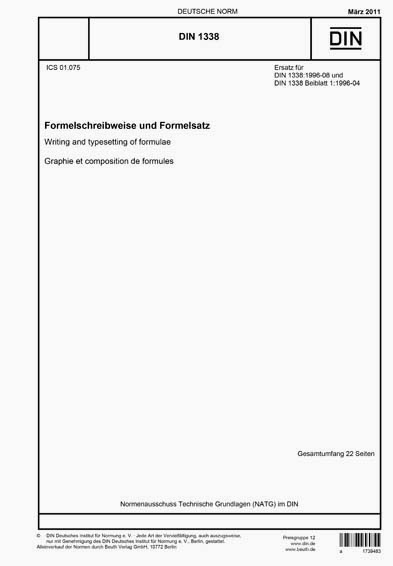
\includegraphics[height=0.25\textwidth]{images/styleguides/din}  &
        
\includegraphics[height=0.25\textwidth]{images/styleguides/iso}    \\[-2ex]
        \tiny\url{apastyle.apa.org}                                      &
        \tiny\url{press.uchicago.edu}                                    &
        \tiny\url{ieee.org}                                              &
        \tiny\url{webstore.ansi.org}                                     &
        \tiny\url{en-standard.eu}
    \end{tabularx}

    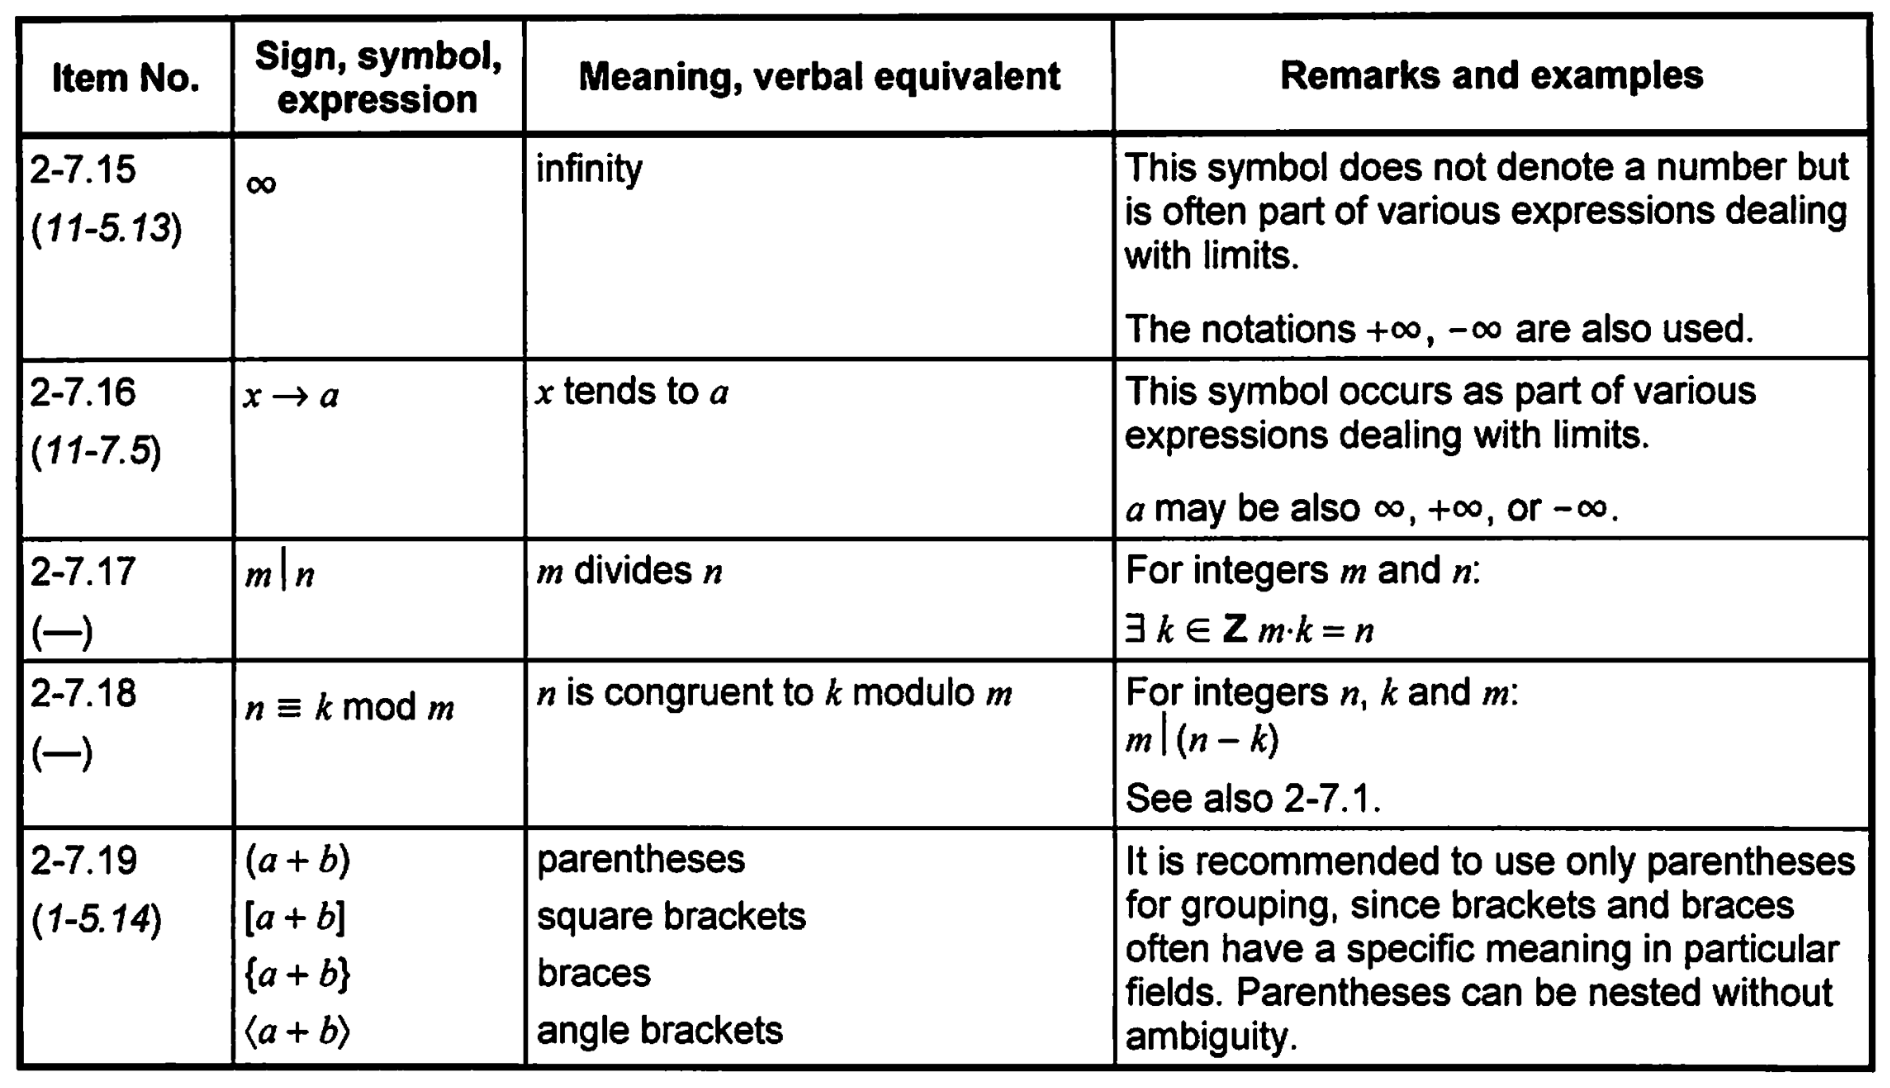
\includegraphics[height=0.32\textwidth]{images/iso-extract}\hfill
    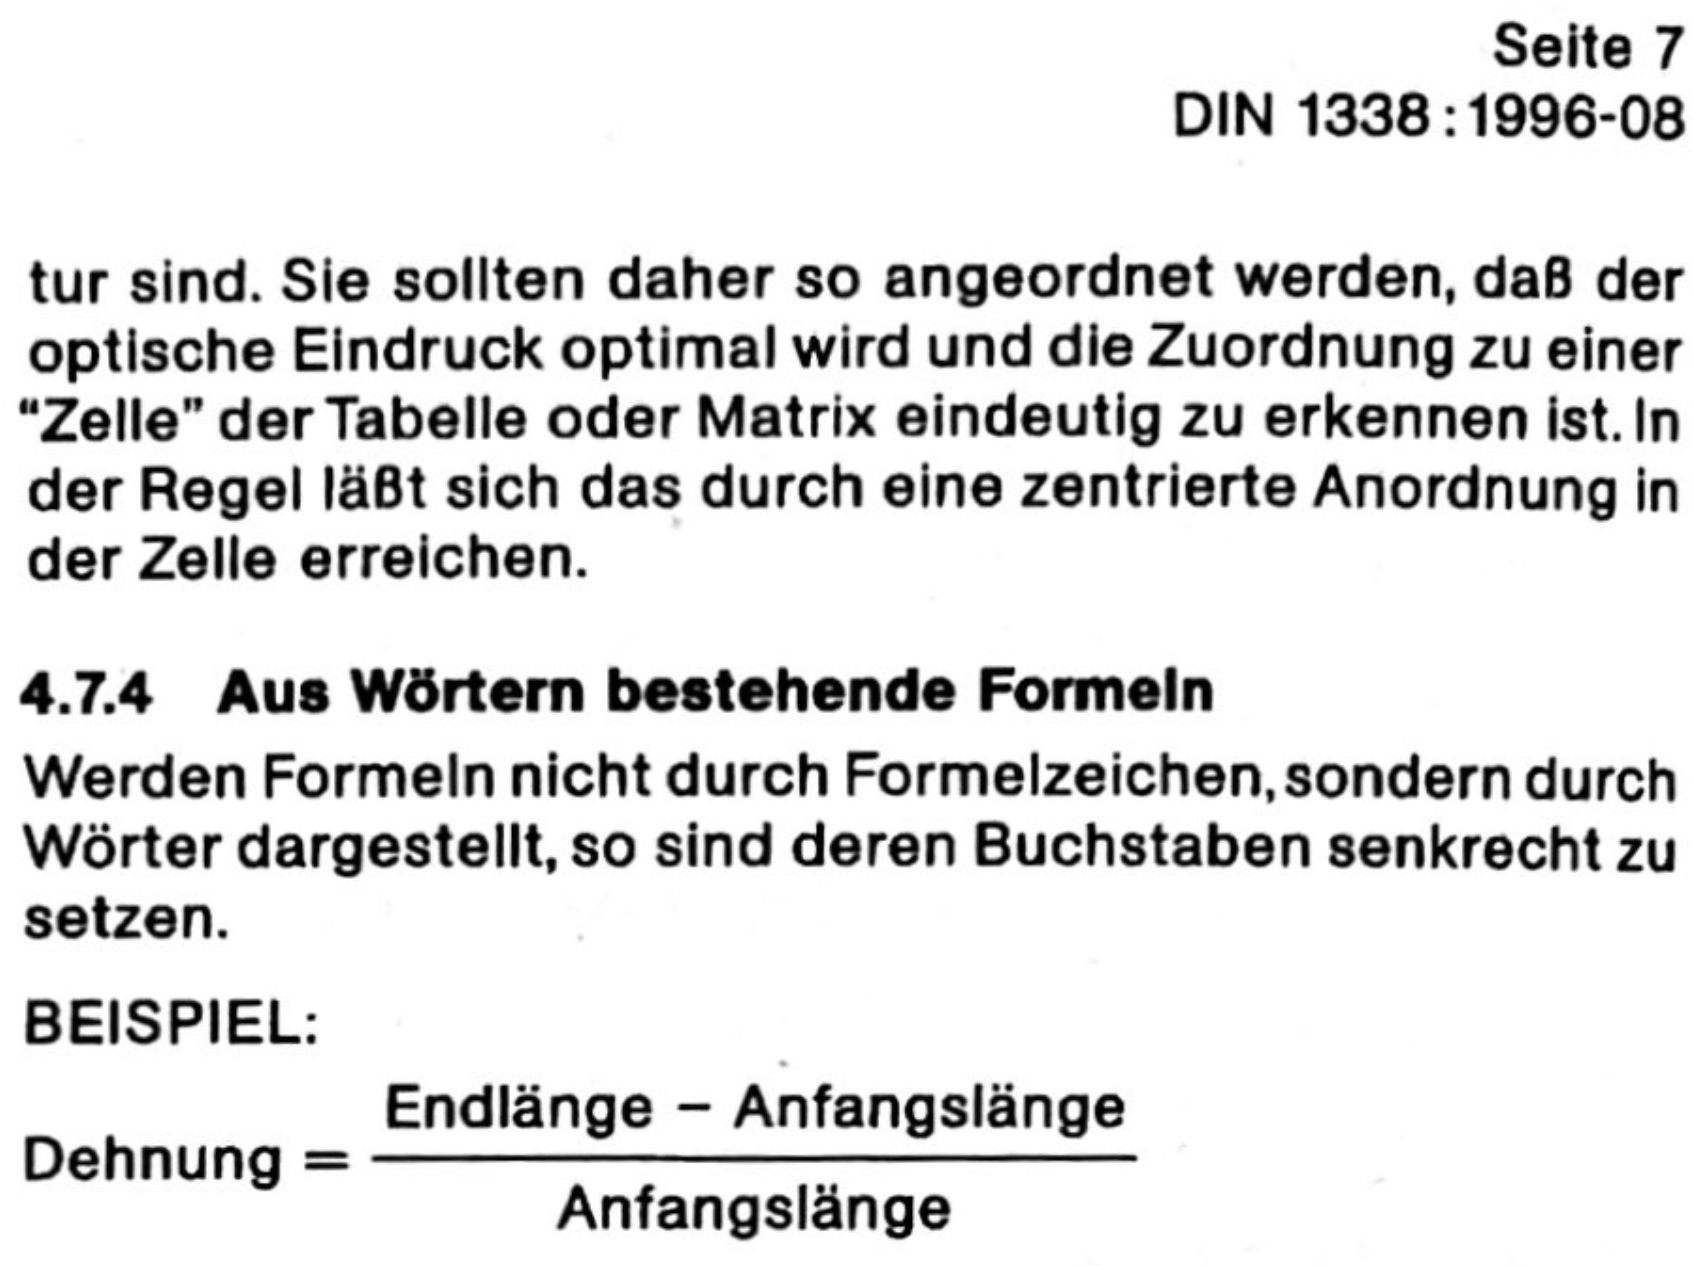
\includegraphics[height=0.32\textwidth]{images/din-extract}
    \note[item]{DIN 1338}
    \note[item]{ISO 80000-2}
\end{frame}

% == == == == == == == == == == == == == == == == == == == == == == == == == == == ==
\section{Mathematische Notation}

\sectiontitlepage

\begin{frame}[fragile]
    \frametitle{Multiplikationspunkt}
    \begin{wrong}
        \begin{lstlisting}
\frac{-b \pm \sqrt{b^2 - 4 * a * c}}{2 * a}
        \end{lstlisting}
    \end{wrong}
    \pause
    \begin{wrong}
        \begin{equation*}
            \frac{-b \pm \sqrt{b^2 - 4 * a * c}}{2 * a}
        \end{equation*}
    \end{wrong}
    \pause
    \begin{lstlisting}
\frac{-b \pm \sqrt{b^2 - 4 \cdot a \cdot c}}{2 \cdot a}
\frac{-b \pm \sqrt{b^2 - 4 a c}}{2 a}
\frac{-b \pm \sqrt{b^2 - 4 \, a \, c}}{2 \, a}
    \end{lstlisting}

    \begin{equation*}
        \frac{-b \pm \sqrt{b^2 - 4 \cdot a \cdot c}}{2 \cdot a}
        \qquad
        \frac{-b \pm \sqrt{b^2 - 4 a c}}{2 a}
        \qquad
        \frac{-b \pm \sqrt{b^2 - 4 \, a \, c}}{2 \, a}
    \end{equation*}
    \pause
    % Hard coded coordinates. I know.
    \begin{tikzpicture}[remember picture, overlay]
        \draw[->, thick, color=markupred] ($(current page.east)-(6em,8ex)$)  node[outer sep=0.2ex,rotate=20,anchor=east] {\Large\bfseries Falsch} to[out=20,in=-100] ($(current page.east) + (-1.6em,1ex)$);
    \end{tikzpicture}
\end{frame}

\begin{frame}[fragile]
    \frametitle{Symbolvarianten}
    \begin{tabularx}{\textwidth}{@{}CCCC@{}}
        \lstinline{\\epsilon} & \lstinline{                                                                                                                                                         \\theta} & \lstinline{\\rho} & \lstinline{\\phi}          \\
        $\mathlarger{\mathlarger{\mathlarger\epsilon}}$ & $\mathlarger{\mathlarger{\mathlarger\theta}}$ & $\mathlarger{\mathlarger{\mathlarger\rho}}$ & $\mathlarger{\mathlarger{\mathlarger\phi}}$ \\
    \end{tabularx}\\[2ex]

    \pause

    \begin{tabularx}{\textwidth}{@{}CCCC@{}}
        \lstinline{\\varepsilon} & \lstinline{                                                                                                                                                                  \\vartheta} & \lstinline{\\varrho} & \lstinline{\\varphi}          \\
        $\mathlarger{\mathlarger{\mathlarger\varepsilon}}$ & $\mathlarger{\mathlarger{\mathlarger\vartheta}}$ & $\mathlarger{\mathlarger{\mathlarger\varrho}}$ & $\mathlarger{\mathlarger{\mathlarger\varphi}}$ \\
    \end{tabularx}
\end{frame}

\begin{frame}[fragile]
    \frametitle{Konventionelle Zeichen}
    \begin{wrong}
        \begin{lstlisting}
x = log_2 n \cdot sin n
sin^2 \theta + cos^2 \theta = 1
        \end{lstlisting}
    \end{wrong}

    \pause

    \begin{wrong}
        \begin{equation*}
            x = log_2 n \cdot sin n \qquad sin^2 \theta + cos^2 \theta = 1
        \end{equation*}
    \end{wrong}\\[2ex]

    \pause

    \begin{lstlisting}
x = \log_2 n \cdot \sin n
\sin^2 \theta + \cos^2 \theta = 1
        \end{lstlisting}
    \begin{equation*}
        x = \log_2 n \cdot \sin n \qquad \sin^2 \theta + \cos^2 \theta = 1
    \end{equation*}\\[2ex]

    \pause

    \begin{lstlisting}
\DeclareMathOperator{\atan}{atan} % Preamble
\DeclareMathOperator*{\argmax}{argmax} % Preamble
\atan x
\argmax_\theta f(x)
        \end{lstlisting}
    \begin{equation*}
        \min \quad \sin \quad \cos \quad \tan \quad \arctan \quad \log \quad \lg \quad \ln \quad \atan x \quad \argmax_\theta f(x)
    \end{equation*}
\end{frame}

\begin{frame}[fragile]
    \frametitle{Indexstellung}%
    \vspace*{-1ex}
    \begin{wrong}
        \begin{lstlisting}[basicstyle=\footnotesize\ttfamily]
v_e=\sqrt{\frac{2GM_{Earth}}{r_{spacecraft}}}
        \end{lstlisting}
        \begin{equation*}
            v_e=\sqrt{\frac{2GM_{Earth}}{r_{spacecraft}}}
        \end{equation*}
    \end{wrong}
    \pause
    \begin{wrong}
        \begin{lstlisting}[basicstyle=\footnotesize\ttfamily]
v_e=\sqrt{\frac{2GM_\mathit{Earth}}{r_\mathit{spacecraft}}}
        \end{lstlisting}
        \begin{equation*}
            v_e=\sqrt{\frac{2GM_\mathit{Earth}}{r_\mathit{spacecraft}}}
        \end{equation*}
    \end{wrong}
    \pause
    \begin{wrong}
        \begin{lstlisting}[basicstyle=\footnotesize\ttfamily]
v_\text{e}=\sqrt{\frac{2GM_\text{Earth}}{r_\text{spacecraft}}}
        \end{lstlisting}
        \begin{equation*}
            v_\text{e}=\sqrt{\frac{2GM_\text{Earth}}{r_\text{spacecraft}}}
        \end{equation*}
    \end{wrong}
    \pause
    \begin{lstlisting}[basicstyle=\footnotesize\ttfamily]
v_\mathrm{e}=\sqrt{\frac{2GM_\mathrm{Earth}}{r_\mathrm{spacecraft}}}
    \end{lstlisting}
    \begin{equation*}
        v_\mathrm{e} = \sqrt{\frac{2GM_\mathrm{Earth}}{r_\mathrm{spacecraft}}}
    \end{equation*}
    \note[item]{Variable vs. Bezeichnung}
    \note[item]{Escape Velocity}
\end{frame}

\begin{frame}[fragile]
    \frametitle{Indexstellung \textsc{ii}}%
    \begin{lstlisting}
\mat a \cdot \mat b = \sum_{i=1}^n a_i b_i
    \end{lstlisting}
    \begin{equation*}
        \mat a \cdot \mat b = \sum_{i=1}^n a_i b_i
    \end{equation*}

    \begin{lstlisting}
a_\mathrm{max} = \max(a_1, \dots, a_n)
    \end{lstlisting}
    \begin{equation*}
        a_\mathrm{max} = \max(a_1, \dots, a_n)
    \end{equation*}

    \begin{lstlisting}
\gamma_\mathrm{n} = \frac{P_\mathrm{s}}{P_\mathrm{n}}
    \end{lstlisting}
    \begin{equation*}
        \gamma_\mathrm{n} = \frac{P_\mathrm{s}}{P_\mathrm{n}}
    \end{equation*}
    \note[item]{SNR = Signal Power / Noise Power}

    \begin{lstlisting}
a_{i, \mathrm{max}}
    \end{lstlisting}
    \begin{equation*}
        a_{i, \mathrm{max}}
    \end{equation*}
\end{frame}

\begin{frame}[fragile]
    \frametitle{Spezielle Konstanten}
    \begin{equation*}
        \mathlarger{\mathlarger{\mathlarger\e^{\pi \i} + 1 = 0}}
    \end{equation*}
    \begin{lstlisting}
\newcommand{\e}{\mathrm{e}} % Preamble
\renewcommand{\i}{\mathrm{i}} % Preamble
    \end{lstlisting}
    ~

    \pause
    Nach \textsc{din} und \textsc{iso} sogar aufrechtes Pi:
    \begin{equation*}
        \mathlarger{\mathlarger{\mathlarger\e^{\mathrm{π} \i} + 1 = 0}}
    \end{equation*}\\[2ex]

    \pause
    Nach \textsc{apa} sind alle griechischen Buchstaben aufrecht zu setzen.\\[2ex]

    \pause
    \LaTeX{} Standard:
    \begin{tabularx}{\textwidth}{@{}C@{}C@{}C@{}C@{}C@{}C@{}C@{}C@{}C@{}C@{}C@{}C@{}C@{}C@{}C@{}C@{}C@{}C@{}C@{}C@{}C@{}C@{}C@{}C@{}}
        $\alpha$ & $\beta$ & $\gamma$ & $\delta$ & $\epsilon$ & $\zeta$ & $\eta$ & $\theta$ & $\iota$ & $\kappa$ & $\lambda$ & $\mu$ & $\nu$ & $\xi$ & $\omicron$ & $\pi$ & $\rho$ & $\sigma$ & $\tau$ & $\upsilon$ & $\phi$ & $\chi$ & $\psi$ & $\omega$ \\
        $\Alpha$ & $\Beta$ & $\Gamma$ & $\Delta$ & $\Epsilon$ & $\Zeta$ & $\Eta$ & $\Theta$ & $\Iota$ & $\Kappa$ & $\Lambda$ & $\Mu$ & $\Nu$ & $\Xi$ & $\Omicron$ & $\Pi$ & $\Rho$ & $\Sigma$ & $\Tau$ & $\Upsilon$ & $\Phi$ & $\Chi$ & $\Psi$ & $\Omega$ \\
    \end{tabularx}
\end{frame}

\begin{frame}[fragile]
    \frametitle{Doch Text in Mathe}
    \begin{lstlisting}
\Lambda(x) = \begin{cases}
    1 - |x| & \text{if\ } |x| < 1 \,, \\
    0       & \text{otherwise}      .
\end{cases}
    \end{lstlisting}
    \begin{equation*}
        \Lambda(x) = \begin{cases}
            1 - |x| & \text{if\ } |x| < 1 \,, \\
            0       & \text{otherwise}      .
        \end{cases}
    \end{equation*}

    \pause

    \begin{lstlisting}
f(n) = \begin{cases}
    n/2\,,    & n \text{ is even} ; \\
    3n + 1\\, & n \text{ is odd}  .
\end{cases}
    \end{lstlisting}
    \begin{equation*}
        f(n) = \begin{cases}
            n/2\,,    & n \text{ is even} ; \\
            3n + 1\,, & n \text{ is odd}  .
        \end{cases}
    \end{equation*}
\end{frame}

\begin{frame}[fragile]
    \frametitle{Vektoren}%
    \begin{lstlisting}
\vec a \cdot \vec b = \sum_{i=1}^n a_i b_i
    \end{lstlisting}
    \begin{equation*}
        \vec a \cdot \vec b = \sum_{i=1}^n a_i b_i
    \end{equation*}

    \pause

    \begin{lstlisting}
\newcommand{\mat}[1]{\mathbfit{#1}} % Preamble
\mat a \cdot \mat b = \sum_{i=1}^n a_i b_i
    \end{lstlisting}
    \begin{equation*}
        \mat a \cdot \mat b = \sum_{i=1}^n a_i b_i
    \end{equation*}

    \pause

    \textbf{Nach \textsc{iso} 80000-2:}
    \begin{itemize}
        \item Skalar $a$\,,
        \item Vektor $\mat a$ oder $\vec a$\,,
        \item Matrix oder Tensor $\mat A$ oder \smash{$\vec{\vec{A}}$}\,,
        \item Vektorelement $a_i$ oder Tensorelement $A_{ij}$\,;
        \item Einheitsvektor in die Richtung von $\mat a$, $\mat e_{\mat a}$\,, aber auch $\mat e_x$\,.
    \end{itemize}
\end{frame}

\begin{frame}[fragile]
    \frametitle{Klammergrößen}%
    \begin{wrong}
        \begin{lstlisting}
t' = \gamma \cdot ( t - \frac{vx}{c^2} )
    \end{lstlisting}
        \begin{equation*}
            t' = \gamma \cdot ( t - \frac{vx}{c^2} )
        \end{equation*}
    \end{wrong}

    \pause

    \begin{lstlisting}
t' = \gamma \cdot \left( t - \frac{vx}{c^2} \right)
    \end{lstlisting}
    \begin{equation*}
        t' = \gamma \cdot \left( t - \frac{vx}{c^2} \right)
    \end{equation*}

    \pause

    \begin{lstlisting}
\Bigg( \bigg( \Big( \big( x \big) \Big) \bigg) \Bigg)
    \end{lstlisting}
    \begin{equation*}
        \Bigg( \bigg( \Big( \big( x \big) \Big) \bigg) \Bigg)
    \end{equation*}

    \pause

    \begin{lstlisting}
f (x + 2) \cdot f \left( \frac{x}{2} + 2 \right)
    \end{lstlisting}
    \begin{equation*}
        f (x + 2) \cdot f \left( \frac{x}{2} + 2 \right) \qquad\pause f (x + 2) \cdot f \mleft( \frac{x}{2} + 2 \mright)
    \end{equation*}%
    \vspace*{-2ex}%
    \begin{lstlisting}
\usepackage{mleftright} % Preamble
f (x + 2) \cdot f \mleft( \frac{x}{2} + 2 \mright)
    \end{lstlisting}
\end{frame}

\begin{frame}[fragile]
    \frametitle{Einheiten}
    \begin{equation*}
        f_\mathrm{laden\:swallow} = f_\mathrm{unladen\:swallow} \cdot \frac{m_\mathrm{coconut} + m_\mathrm{unladen\:swallow}}{m_\mathrm{unladen\:swallow}}
    \end{equation*}
    \pause
    \begin{wrong}
        \begin{lstlisting}
43bps \cdot \frac{500g + 150g}{150g} \approx 186.3bps
        \end{lstlisting}
        \begin{equation*}
            43 bps \cdot \frac{500 g + 150 g}{150 g} \approx 186.3 bps
        \end{equation*}
    \end{wrong}
    \pause
    \DeclareSIUnit{\beat}{b}
    \begin{lstlisting}
\usepackage{siunitx} % Preamble
\DeclareSIUnit{\beat}{b} % Preamble
\qty{43}{\beat\per\second} \cdot \frac{
    \qty{500}{\gram} + \qty{150}{\gram}}{\qty{150}{\gram}}
    \approx \qty{186.3}{\beat\per\second}
    \approx \qty{0.2}{\kilo\hertz}
        \end{lstlisting}
    \begin{equation*}
        \qty{43}{\beat\per\second} \cdot \frac{\qty{500}{\gram} + \qty{150}{\gram}}{\qty{150}{\gram}} \approx \qty{186.3}{\beat\per\second} \approx \qty{0.2}{\kilo\hertz}
    \end{equation*}
\end{frame}

\begin{frame}[fragile]
    \frametitle{Einheiten \textsc{ii}}
    \begin{wrong}
        Bitte berechnen Sie $v$ $[\unit{\meter\per\second}]$.
    \end{wrong}
    \pause
    Bitte berechnen Sie $v$ in \unit{\meter\per\second}.
    \pause
    \begin{equation*}
        Q = \{Q\} \cdot [Q]
    \end{equation*}
    \note[item]{Größe $Q$}
    \note[item]{numerische Wert der Größe}
    \note[item]{Einheit}
    \pause
    \begin{equation*}
        [m] = \unit{\kilo\gram}
    \end{equation*}
    \pause
    \begin{multicols}{2}
        % This file was created with tikzplotlib v0.9.15.
\begin{tikzpicture}

    \begin{axis}[
            xmin=0, xmax=11,
            width=\linewidth,
            height=0.4\paperheight,
            ylabel={$v\,[\unit{\meter\per\second}]$},
            xlabel={$t\,[\unit{\second}]$},
        ]
        \addplot [very thick]
        table {%
                0 0
                0.01 0.0164282196969697
                0.02 0.0327583333333333
                0.03 0.0489903409090909
                0.04 0.0651242424242424
                0.05 0.0811600378787879
                0.06 0.0970977272727273
                0.07 0.112937310606061
                0.08 0.128678787878788
                0.09 0.144322159090909
                0.1 0.159867424242424
                0.11 0.175314583333333
                0.12 0.190663636363636
                0.13 0.205914583333333
                0.14 0.221067424242424
                0.15 0.236122159090909
                0.16 0.251078787878788
                0.17 0.265937310606061
                0.18 0.280697727272727
                0.19 0.295360037878788
                0.2 0.309924242424242
                0.21 0.324390340909091
                0.22 0.338758333333333
                0.23 0.35302821969697
                0.24 0.3672
                0.25 0.381273674242424
                0.26 0.395249242424242
                0.27 0.409126704545455
                0.28 0.422906060606061
                0.29 0.436587310606061
                0.3 0.450170454545455
                0.31 0.463655492424242
                0.32 0.477042424242424
                0.33 0.49033125
                0.34 0.50352196969697
                0.35 0.516614583333333
                0.36 0.529609090909091
                0.37 0.542505492424242
                0.38 0.555303787878788
                0.39 0.568003977272727
                0.4 0.580606060606061
                0.41 0.593110037878788
                0.42 0.605515909090909
                0.43 0.617823674242424
                0.44 0.630033333333333
                0.45 0.642144886363636
                0.46 0.654158333333333
                0.47 0.666073674242424
                0.48 0.677890909090909
                0.49 0.689610037878788
                0.5 0.701231060606061
                0.51 0.712753977272727
                0.52 0.724178787878788
                0.53 0.735505492424242
                0.54 0.746734090909091
                0.55 0.757864583333333
                0.56 0.76889696969697
                0.57 0.77983125
                0.58 0.790667424242424
                0.59 0.801405492424242
                0.6 0.812045454545454
                0.61 0.822587310606061
                0.62 0.83303106060606
                0.63 0.843376704545455
                0.64 0.853624242424242
                0.65 0.863773674242424
                0.66 0.873825
                0.67 0.88377821969697
                0.68 0.893633333333333
                0.69 0.903390340909091
                0.7 0.913049242424242
                0.71 0.922610037878788
                0.72 0.932072727272727
                0.73 0.941437310606061
                0.74 0.950703787878788
                0.75 0.959872159090909
                0.76 0.968942424242424
                0.77 0.977914583333333
                0.78 0.986788636363636
                0.79 0.995564583333333
                0.8 1.00424242424242
                0.81 1.01282215909091
                0.82 1.02130378787879
                0.83 1.02968731060606
                0.84 1.03797272727273
                0.85 1.04616003787879
                0.86 1.05424924242424
                0.87 1.06224034090909
                0.88 1.07013333333333
                0.89 1.07792821969697
                0.9 1.085625
                0.91 1.09322367424242
                0.92 1.10072424242424
                0.93 1.10812670454545
                0.94 1.11543106060606
                0.95 1.12263731060606
                0.96 1.12974545454545
                0.97 1.13675549242424
                0.98 1.14366742424242
                0.99 1.15048125
                1 1.15719696969697
                1.01 1.16381458333333
                1.02 1.17033409090909
                1.03 1.17675549242424
                1.04 1.18307878787879
                1.05 1.18930397727273
                1.06 1.19543106060606
                1.07 1.20146003787879
                1.08 1.20739090909091
                1.09 1.21322367424242
                1.1 1.21895833333333
                1.11 1.22459488636364
                1.12 1.23013333333333
                1.13 1.23557367424242
                1.14 1.24091590909091
                1.15 1.24616003787879
                1.16 1.25130606060606
                1.17 1.25635397727273
                1.18 1.26130378787879
                1.19 1.26615549242424
                1.2 1.27090909090909
                1.21 1.27556458333333
                1.22 1.28012196969697
                1.23 1.28458125
                1.24 1.28894242424242
                1.25 1.29320549242424
                1.26 1.29737045454545
                1.27 1.30143731060606
                1.28 1.30540606060606
                1.29 1.30927670454545
                1.3 1.31304924242424
                1.31 1.31672367424242
                1.32 1.3203
                1.33 1.32377821969697
                1.34 1.32715833333333
                1.35 1.33044034090909
                1.36 1.33362424242424
                1.37 1.33671003787879
                1.38 1.33969772727273
                1.39 1.34258731060606
                1.4 1.34537878787879
                1.41 1.34807215909091
                1.42 1.35066742424242
                1.43 1.35316458333333
                1.44 1.35556363636364
                1.45 1.35786458333333
                1.46 1.36006742424242
                1.47 1.36217215909091
                1.48 1.36417878787879
                1.49 1.36608731060606
                1.5 1.36789772727273
                1.51 1.36961003787879
                1.52 1.37122424242424
                1.53 1.37274034090909
                1.54 1.37415833333333
                1.55 1.37547821969697
                1.56 1.3767
                1.57 1.37782367424242
                1.58 1.37884924242424
                1.59 1.37977670454545
                1.6 1.38060606060606
                1.61 1.38133731060606
                1.62 1.38197045454545
                1.63 1.38250549242424
                1.64 1.38294242424242
                1.65 1.38328125
                1.66 1.38352196969697
                1.67 1.38366458333333
                1.68 1.38370909090909
                1.69 1.38365549242424
                1.7 1.38350378787879
                1.71 1.38325397727273
                1.72 1.38290606060606
                1.73 1.38246003787879
                1.74 1.38191590909091
                1.75 1.38127367424242
                1.76 1.38053333333333
                1.77 1.37969488636364
                1.78 1.37875833333333
                1.79 1.37772367424242
                1.8 1.37659090909091
                1.81 1.37536003787879
                1.82 1.37403106060606
                1.83 1.37260397727273
                1.84 1.37107878787879
                1.85 1.36945549242424
                1.86 1.36773409090909
                1.87 1.36591458333333
                1.88 1.36399696969697
                1.89 1.36198125
                1.9 1.35986742424242
                1.91 1.35765549242424
                1.92 1.35534545454545
                1.93 1.35293731060606
                1.94 1.35043106060606
                1.95 1.34782670454545
                1.96 1.34512424242424
                1.97 1.34232367424242
                1.98 1.339425
                1.99 1.33642821969697
                2 1.33333333333333
                2.01 1.33014034090909
                2.02 1.32684924242424
                2.03 1.32346003787879
                2.04 1.31997272727273
                2.05 1.31638731060606
                2.06 1.31270378787879
                2.07 1.30892215909091
                2.08 1.30504242424242
                2.09 1.30106458333333
                2.1 1.29698863636364
                2.11 1.29281458333333
                2.12 1.28854242424242
                2.13 1.28417215909091
                2.14 1.27970378787879
                2.15 1.27513731060606
                2.16 1.27047272727273
                2.17 1.26571003787879
                2.18 1.26084924242424
                2.19 1.25589034090909
                2.2 1.25083333333333
                2.21 1.24567821969697
                2.22 1.240425
                2.23 1.23507367424242
                2.24 1.22962424242424
                2.25 1.22407670454545
                2.26 1.21843106060606
                2.27 1.21268731060606
                2.28 1.20684545454545
                2.29 1.20090549242424
                2.3 1.19486742424242
                2.31 1.18873125
                2.32 1.18249696969697
                2.33 1.17616458333333
                2.34 1.16973409090909
                2.35 1.16320549242424
                2.36 1.15657878787879
                2.37 1.14985397727273
                2.38 1.14303106060606
                2.39 1.13611003787879
                2.4 1.12909090909091
                2.41 1.12197367424242
                2.42 1.11475833333333
                2.43 1.10744488636364
                2.44 1.10003333333333
                2.45 1.09252367424242
                2.46 1.08491590909091
                2.47 1.07721003787879
                2.48 1.06940606060606
                2.49 1.06150397727273
                2.5 1.05350378787879
                2.51 1.04540549242424
                2.52 1.03720909090909
                2.53 1.02891458333333
                2.54 1.02052196969697
                2.55 1.01203125
                2.56 1.00344242424242
                2.57 0.994755492424242
                2.58 0.985970454545454
                2.59 0.97708731060606
                2.6 0.96810606060606
                2.61 0.959026704545454
                2.62 0.949849242424242
                2.63 0.940573674242424
                2.64 0.9312
                2.65 0.921728219696969
                2.66 0.912158333333332
                2.67 0.902490340909091
                2.68 0.892724242424241
                2.69 0.882860037878788
                2.7 0.872897727272727
                2.71 0.86283731060606
                2.72 0.852678787878787
                2.73 0.842422159090908
                2.74 0.832067424242423
                2.75 0.821614583333333
                2.76 0.811063636363635
                2.77 0.800414583333333
                2.78 0.789667424242424
                2.79 0.778822159090908
                2.8 0.767878787878787
                2.81 0.75683731060606
                2.82 0.745697727272727
                2.83 0.734460037878787
                2.84 0.723124242424242
                2.85 0.71169034090909
                2.86 0.700158333333333
                2.87 0.68852821969697
                2.88 0.676799999999999
                2.89 0.664973674242423
                2.9 0.653049242424242
                2.91 0.641026704545453
                2.92 0.62890606060606
                2.93 0.61668731060606
                2.94 0.604370454545454
                2.95 0.591955492424242
                2.96 0.579442424242424
                2.97 0.566831249999998
                2.98 0.554121969696969
                2.99 0.541314583333333
                3 0.528409090909091
                3.01 0.515469912997159
                3.02 0.502561470170455
                3.03 0.489683762428978
                3.04 0.476836789772728
                3.05 0.464020552201706
                3.06 0.451235049715911
                3.07 0.438480282315343
                3.08 0.425756250000002
                3.09 0.413062952769889
                3.1 0.400400390625003
                3.11 0.387768563565344
                3.12 0.375167471590912
                3.13 0.362597114701708
                3.14 0.350057492897731
                3.15 0.337548606178981
                3.16 0.325070454545459
                3.17 0.312623037997164
                3.18 0.300206356534096
                3.19 0.287820410156255
                3.2 0.275465198863642
                3.21 0.263140722656256
                3.22 0.250846981534097
                3.23 0.238583975497165
                3.23999999999999 0.226351704545461
                3.24999999999999 0.214150168678984
                3.25999999999999 0.201979367897734
                3.26999999999999 0.189839302201712
                3.27999999999999 0.177729971590916
                3.28999999999999 0.165651376065348
                3.29999999999999 0.153603515625008
                3.30999999999999 0.141586390269894
                3.31999999999999 0.129600000000008
                3.32999999999999 0.117644344815349
                3.33999999999999 0.105719424715918
                3.34999999999999 0.0938252397017135
                3.35999999999999 0.0819617897727364
                3.36999999999999 0.0701290749289866
                3.37999999999999 0.0583270951704641
                3.38999999999999 0.0465558504971689
                3.39999999999999 0.034815340909101
                3.40999999999999 0.0231055664062603
                3.41999999999999 0.0114265269886468
                3.42999999999999 -0.000221777343739293
                3.43999999999999 -0.0118393465908981
                3.44999999999999 -0.0234261807528298
                3.45999999999999 -0.0349822798295341
                3.46999999999999 -0.0465076438210111
                3.47999999999999 -0.0580022727272609
                3.48999999999999 -0.0694661665482834
                3.49999999999999 -0.0808993252840787
                3.50999999999999 -0.0923017489346466
                3.51999999999999 -0.103673437499987
                3.52999999999999 -0.115014390980101
                3.53999999999999 -0.126324609374987
                3.54999999999999 -0.137604092684646
                3.55999999999999 -0.148852840909077
                3.56999999999999 -0.160070854048282
                3.57999999999999 -0.171258132102259
                3.58999999999999 -0.182414675071009
                3.59999999999999 -0.193540482954531
                3.60999999999999 -0.204635555752826
                3.61999999999999 -0.215699893465894
                3.62999999999999 -0.226733496093735
                3.63999999999999 -0.237736363636349
                3.64999999999999 -0.248708496093735
                3.65999999999999 -0.259649893465894
                3.66999999999999 -0.270560555752825
                3.67999999999999 -0.28144048295453
                3.68999999999999 -0.292289675071007
                3.69999999999999 -0.303108132102257
                3.70999999999998 -0.313895854048279
                3.71999999999998 -0.324652840909074
                3.72999999999998 -0.335379092684642
                3.73999999999998 -0.346074609374983
                3.74999999999998 -0.356739390980097
                3.75999999999998 -0.367373437499983
                3.76999999999998 -0.377976748934642
                3.77999999999998 -0.388549325284073
                3.78999999999998 -0.399091166548278
                3.79999999999998 -0.409602272727255
                3.80999999999998 -0.420082643821005
                3.81999999999998 -0.430532279829527
                3.82999999999998 -0.440951180752822
                3.83999999999998 -0.451339346590891
                3.84999999999998 -0.461696777343731
                3.85999999999998 -0.472023473011345
                3.86999999999998 -0.482319433593731
                3.87999999999998 -0.49258465909089
                3.88999999999998 -0.502819149502821
                3.89999999999998 -0.513022904829526
                3.90999999999998 -0.523195925071003
                3.91999999999998 -0.533338210227253
                3.92999999999998 -0.543449760298275
                3.93999999999998 -0.553530575284071
                3.94999999999998 -0.563580655184639
                3.95999999999998 -0.573599999999979
                3.96999999999998 -0.583588609730093
                3.97999999999998 -0.593546484374979
                3.98999999999998 -0.603473623934638
                3.99999999999998 -0.61337002840907
                4.00999999999998 -0.623235697798274
                4.01999999999998 -0.633070632102251
                4.02999999999998 -0.642874831321001
                4.03999999999998 -0.652648295454524
                4.04999999999998 -0.662391024502819
                4.05999999999998 -0.672103018465887
                4.06999999999998 -0.681784277343728
                4.07999999999998 -0.691434801136341
                4.08999999999998 -0.701054589843728
                4.09999999999998 -0.710643643465887
                4.10999999999998 -0.720201962002818
                4.11999999999998 -0.729729545454523
                4.12999999999998 -0.739226393821
                4.13999999999998 -0.74869250710225
                4.14999999999998 -0.758127885298272
                4.15999999999998 -0.767532528409068
                4.16999999999998 -0.776906436434636
                4.17999999999997 -0.786249609374976
                4.18999999999997 -0.79556204723009
                4.19999999999997 -0.804843749999976
                4.20999999999997 -0.814094717684635
                4.21999999999997 -0.823314950284067
                4.22999999999997 -0.832504447798271
                4.23999999999997 -0.841663210227248
                4.24999999999997 -0.850791237570998
                4.25999999999997 -0.859888529829521
                4.26999999999997 -0.868955087002816
                4.27999999999997 -0.877990909090884
                4.28999999999997 -0.886995996093725
                4.29999999999997 -0.895970348011339
                4.30999999999997 -0.904913964843725
                4.31999999999997 -0.913826846590884
                4.32999999999997 -0.922708993252816
                4.33999999999997 -0.93156040482952
                4.34999999999997 -0.940381081320997
                4.35999999999997 -0.949171022727247
                4.36999999999997 -0.95793022904827
                4.37999999999997 -0.966658700284065
                4.38999999999997 -0.975356436434633
                4.39999999999997 -0.984023437499974
                4.40999999999997 -0.992659703480088
                4.41999999999997 -1.00126523437497
                4.42999999999997 -1.00984003018463
                4.43999999999997 -1.01838409090906
                4.44999999999997 -1.02689741654827
                4.45999999999997 -1.03538000710225
                4.46999999999997 -1.043831862571
                4.47999999999997 -1.05225298295452
                4.48999999999997 -1.06064336825281
                4.49999999999997 -1.06900301846588
                4.50999999999997 -1.07733193359372
                4.51999999999997 -1.08563011363634
                4.52999999999997 -1.09389755859372
                4.53999999999997 -1.10213426846588
                4.54999999999997 -1.11034024325281
                4.55999999999997 -1.11851548295452
                4.56999999999997 -1.126659987571
                4.57999999999997 -1.13477375710225
                4.58999999999997 -1.14285679154827
                4.59999999999997 -1.15090909090906
                4.60999999999997 -1.15893065518463
                4.61999999999997 -1.16692148437497
                4.62999999999997 -1.17488157848009
                4.63999999999997 -1.18281093749997
                4.64999999999996 -1.19070956143463
                4.65999999999996 -1.19857745028406
                4.66999999999996 -1.20641460404827
                4.67999999999996 -1.21422102272724
                4.68999999999996 -1.22199670632099
                4.69999999999996 -1.22974165482952
                4.70999999999996 -1.23745586825281
                4.71999999999996 -1.24513934659088
                4.72999999999996 -1.25279208984372
                4.73999999999996 -1.26041409801134
                4.74999999999996 -1.26800537109372
                4.75999999999996 -1.27556590909088
                4.76999999999996 -1.28309571200281
                4.77999999999996 -1.29059477982952
                4.78999999999996 -1.29806311257099
                4.79999999999996 -1.30550071022724
                4.80999999999996 -1.31290757279827
                4.81999999999996 -1.32028370028406
                4.82999999999996 -1.32762909268463
                4.83999999999996 -1.33494374999997
                4.84999999999996 -1.34222767223008
                4.85999999999996 -1.34948085937497
                4.86999999999996 -1.35670331143463
                4.87999999999996 -1.36389502840906
                4.88999999999996 -1.37105601029827
                4.89999999999996 -1.37818625710224
                4.90999999999996 -1.38528576882099
                4.91999999999996 -1.39235454545452
                4.92999999999996 -1.39939258700281
                4.93999999999996 -1.40639989346588
                4.94999999999996 -1.41337646484372
                4.95999999999996 -1.42032230113633
                4.96999999999996 -1.42723740234372
                4.97999999999996 -1.43412176846588
                4.98999999999996 -1.44097539950281
                4.99999999999996 -1.44779829545452
                5.00999999999996 -1.45459045632099
                5.01999999999996 -1.46135188210224
                5.02999999999996 -1.46808257279827
                5.03999999999996 -1.47478252840906
                5.04999999999996 -1.48145174893463
                5.05999999999996 -1.48809023437497
                5.06999999999996 -1.49469798473008
                5.07999999999996 -1.50127499999997
                5.08999999999996 -1.50782128018463
                5.09999999999996 -1.51433682528406
                5.10999999999996 -1.52082163529827
                5.11999999999995 -1.52727571022724
                5.12999999999995 -1.53369905007099
                5.13999999999995 -1.54009165482952
                5.14999999999995 -1.54645352450281
                5.15999999999995 -1.55278465909088
                5.16999999999995 -1.55908505859372
                5.17999999999995 -1.56535472301133
                5.18999999999995 -1.57159365234372
                5.19999999999995 -1.57780184659088
                5.20999999999995 -1.58397930575281
                5.21999999999995 -1.59012602982952
                5.22999999999995 -1.59624201882099
                5.23999999999995 -1.60232727272724
                5.24999999999995 -1.60838179154827
                5.25999999999995 -1.61440557528406
                5.26999999999995 -1.62039862393463
                5.27999999999995 -1.62636093749997
                5.28999999999995 -1.63229251598008
                5.29999999999995 -1.63819335937497
                5.30999999999995 -1.64406346768463
                5.31999999999995 -1.64990284090906
                5.32999999999995 -1.65571147904827
                5.33999999999995 -1.66148938210224
                5.34999999999995 -1.66723655007099
                5.35999999999995 -1.67295298295452
                5.36999999999995 -1.67863868075281
                5.37999999999995 -1.68429364346588
                5.38999999999995 -1.68991787109372
                5.39999999999995 -1.69551136363634
                5.40999999999995 -1.70107412109372
                5.41999999999995 -1.70660614346588
                5.42999999999995 -1.71210743075281
                5.43999999999995 -1.71757798295452
                5.44999999999995 -1.72301780007099
                5.45999999999995 -1.72842688210224
                5.46999999999995 -1.73380522904827
                5.47999999999995 -1.73915284090906
                5.48999999999995 -1.74446971768463
                5.49999999999995 -1.74975585937497
                5.50999999999995 -1.75501126598009
                5.51999999999995 -1.76023593749997
                5.52999999999995 -1.76542987393463
                5.53999999999995 -1.77059307528406
                5.54999999999995 -1.77572554154827
                5.55999999999995 -1.78082727272724
                5.56999999999995 -1.78589826882099
                5.57999999999995 -1.79093852982952
                5.58999999999994 -1.79594805575281
                5.59999999999994 -1.80092684659088
                5.60999999999994 -1.80587490234372
                5.61999999999994 -1.81079222301134
                5.62999999999994 -1.81567880859372
                5.63999999999994 -1.82053465909088
                5.64999999999994 -1.82535977450281
                5.65999999999994 -1.83015415482952
                5.66999999999994 -1.834917800071
                5.67999999999994 -1.83965071022725
                5.68999999999994 -1.84435288529827
                5.69999999999994 -1.84902432528406
                5.70999999999994 -1.85366503018463
                5.71999999999994 -1.85827499999997
                5.72999999999994 -1.86285423473009
                5.73999999999994 -1.86740273437497
                5.74999999999994 -1.87192049893463
                5.75999999999994 -1.87640752840906
                5.76999999999994 -1.88086382279827
                5.77999999999994 -1.88528938210225
                5.78999999999994 -1.889684206321
                5.79999999999994 -1.89404829545452
                5.80999999999994 -1.89838164950281
                5.81999999999994 -1.90268426846588
                5.82999999999994 -1.90695615234372
                5.83999999999994 -1.91119730113634
                5.84999999999994 -1.91540771484372
                5.85999999999994 -1.91958739346588
                5.86999999999994 -1.92373633700282
                5.87999999999994 -1.92785454545452
                5.88999999999994 -1.931942018821
                5.89999999999994 -1.93599875710225
                5.90999999999994 -1.94002476029827
                5.91999999999994 -1.94402002840907
                5.92999999999994 -1.94798456143463
                5.93999999999994 -1.95191835937498
                5.94999999999994 -1.95582142223009
                5.95999999999994 -1.95969374999998
                5.96999999999994 -1.96353534268463
                5.97999999999994 -1.96734620028407
                5.98999999999994 -1.97112632279827
                5.99999999999994 -1.97487571022725
                6.00999999999994 -1.978594362571
                6.01999999999994 -1.98228227982952
                6.02999999999994 -1.98593946200282
                6.03999999999994 -1.98956590909089
                6.04999999999993 -1.99316162109373
                6.05999999999993 -1.99672659801134
                6.06999999999993 -2.00026083984373
                6.07999999999993 -2.00376434659089
                6.08999999999993 -2.00723711825282
                6.09999999999993 -2.01067915482952
                6.10999999999993 -2.014090456321
                6.11999999999993 -2.01747102272725
                6.12999999999993 -2.02082085404827
                6.13999999999993 -2.02413995028407
                6.14999999999993 -2.02742831143464
                6.15999999999993 -2.03068593749998
                6.16999999999993 -2.03391282848009
                6.17999999999993 -2.03710898437498
                6.18999999999993 -2.04027440518464
                6.19999999999993 -2.04340909090907
                6.20999999999993 -2.04651304154827
                6.21999999999993 -2.04958625710225
                6.22999999999993 -2.052628737571
                6.23999999999993 -2.05564048295452
                6.24999999999993 -2.05862149325282
                6.25999999999993 -2.06157176846589
                6.26999999999993 -2.06449130859373
                6.27999999999993 -2.06738011363634
                6.28999999999993 -2.07023818359373
                6.29999999999993 -2.07306551846589
                6.30999999999993 -2.07586211825282
                6.31999999999993 -2.07862798295453
                6.32999999999993 -2.081363112571
                6.33999999999993 -2.08406750710225
                6.34999999999993 -2.08674116654828
                6.35999999999993 -2.08938409090907
                6.36999999999993 -2.09199628018464
                6.37999999999993 -2.09457773437498
                6.38999999999993 -2.09712845348009
                6.39999999999993 -2.09964843749998
                6.40999999999993 -2.10213768643464
                6.41999999999993 -2.10459620028407
                6.42999999999993 -2.10702397904828
                6.43999999999993 -2.10942102272725
                6.44999999999993 -2.111787331321
                6.45999999999993 -2.11412290482953
                6.46999999999993 -2.11642774325282
                6.47999999999993 -2.11870184659089
                6.48999999999993 -2.12094521484373
                6.49999999999993 -2.12315784801135
                6.50999999999993 -2.12533974609373
                6.51999999999992 -2.12749090909089
                6.52999999999992 -2.12961133700282
                6.53999999999992 -2.13170102982953
                6.54999999999992 -2.13375998757101
                6.55999999999992 -2.13578821022726
                6.56999999999992 -2.13778569779828
                6.57999999999992 -2.13975245028408
                6.58999999999992 -2.14168846768464
                6.59999999999992 -2.14359374999998
                6.60999999999992 -2.1454682972301
                6.61999999999992 -2.14731210937499
                6.62999999999992 -2.14912518643464
                6.63999999999992 -2.15090752840908
                6.64999999999992 -2.15265913529828
                6.65999999999992 -2.15438000710226
                6.66999999999992 -2.15607014382101
                6.67999999999992 -2.15772954545453
                6.68999999999992 -2.15935821200283
                6.69999999999992 -2.1609561434659
                6.70999999999992 -2.16252333984374
                6.71999999999992 -2.16405980113635
                6.72999999999992 -2.16556552734374
                6.73999999999992 -2.1670405184659
                6.74999999999992 -2.16848477450283
                6.75999999999992 -2.16989829545453
                6.76999999999992 -2.17128108132101
                6.77999999999992 -2.17263313210226
                6.78999999999992 -2.17395444779828
                6.79999999999992 -2.17524502840908
                6.80999999999992 -2.17650487393465
                6.81999999999992 -2.17773398437499
                6.82999999999992 -2.1789323597301
                6.83999999999992 -2.18009999999999
                6.84999999999992 -2.18123690518465
                6.85999999999992 -2.18234307528408
                6.86999999999992 -2.18341851029829
                6.87999999999992 -2.18446321022726
                6.88999999999992 -2.18547717507101
                6.89999999999992 -2.18646040482954
                6.90999999999992 -2.18741289950283
                6.91999999999992 -2.1883346590909
                6.92999999999992 -2.18922568359374
                6.93999999999992 -2.19008597301136
                6.94999999999992 -2.19091552734374
                6.95999999999992 -2.1917143465909
                6.96999999999992 -2.19248243075283
                6.97999999999992 -2.19321977982954
                6.98999999999991 -2.19392639382102
                6.99999999999991 -2.19460227272727
                7.00999999999991 -2.19524741654829
                7.01999999999991 -2.19586182528409
                7.02999999999991 -2.19644549893465
                7.03999999999991 -2.19699843749999
                7.04999999999991 -2.19752064098011
                7.05999999999991 -2.198012109375
                7.06999999999991 -2.19847284268465
                7.07999999999991 -2.19890284090909
                7.08999999999991 -2.19930210404829
                7.09999999999991 -2.19967063210227
                7.10999999999991 -2.20000842507102
                7.11999999999991 -2.20031548295454
                7.12999999999991 -2.20059180575284
                7.13999999999991 -2.20083739346591
                7.14999999999991 -2.20105224609375
                7.15999999999991 -2.20123636363636
                7.16999999999991 -2.20138974609375
                7.17999999999991 -2.20151239346591
                7.18999999999991 -2.20160430575284
                7.19999999999991 -2.20166548295455
                7.20999999999991 -2.20169592507102
                7.21999999999991 -2.20169563210227
                7.22999999999991 -2.2016646040483
                7.23999999999991 -2.20160284090909
                7.24999999999991 -2.20151034268466
                7.25999999999991 -2.201387109375
                7.26999999999991 -2.20123314098011
                7.27999999999991 -2.2010484375
                7.28999999999991 -2.20083299893466
                7.29999999999991 -2.20058682528409
                7.30999999999991 -2.2003099165483
                7.31999999999991 -2.20000227272727
                7.32999999999991 -2.19966389382103
                7.33999999999991 -2.19929477982955
                7.34999999999991 -2.19889493075284
                7.35999999999991 -2.19846434659091
                7.36999999999991 -2.19800302734375
                7.37999999999991 -2.19751097301137
                7.38999999999991 -2.19698818359376
                7.39999999999991 -2.19643465909091
                7.40999999999991 -2.19585039950285
                7.41999999999991 -2.19523540482955
                7.42999999999991 -2.19458967507103
                7.43999999999991 -2.19391321022728
                7.44999999999991 -2.1932060102983
                7.4599999999999 -2.1924680752841
                7.4699999999999 -2.19169940518467
                7.4799999999999 -2.19090000000001
                7.4899999999999 -2.19006985973012
                7.4999999999999 -2.18920898437501
                7.5099999999999 -2.18831737393467
                7.5199999999999 -2.1873950284091
                7.5299999999999 -2.1864419477983
                7.5399999999999 -2.18545813210228
                7.5499999999999 -2.18444358132103
                7.5599999999999 -2.18339829545456
                7.5699999999999 -2.18232227450285
                7.5799999999999 -2.18121551846592
                7.5899999999999 -2.18007802734376
                7.5999999999999 -2.17890980113638
                7.6099999999999 -2.17771083984376
                7.6199999999999 -2.17648114346592
                7.6299999999999 -2.17522071200285
                7.6399999999999 -2.17392954545456
                7.6499999999999 -2.17260764382104
                7.6599999999999 -2.17125500710229
                7.6699999999999 -2.16987163529831
                7.6799999999999 -2.16845752840911
                7.6899999999999 -2.16701268643467
                7.6999999999999 -2.16553710937501
                7.7099999999999 -2.16403079723013
                7.7199999999999 -2.16249375000001
                7.7299999999999 -2.16092596768467
                7.7399999999999 -2.15932745028411
                7.7499999999999 -2.15769819779831
                7.7599999999999 -2.15603821022729
                7.7699999999999 -2.15434748757104
                7.7799999999999 -2.15262602982956
                7.7899999999999 -2.15087383700286
                7.7999999999999 -2.14909090909093
                7.8099999999999 -2.14727724609377
                7.8199999999999 -2.14543284801138
                7.8299999999999 -2.14355771484377
                7.8399999999999 -2.14165184659093
                7.8499999999999 -2.13971524325286
                7.8599999999999 -2.13774790482957
                7.8699999999999 -2.13574983132104
                7.8799999999999 -2.13372102272729
                7.8899999999999 -2.13166147904832
                7.8999999999999 -2.12957120028411
                7.9099999999999 -2.12745018643468
                7.9199999999999 -2.12529843750002
                7.92999999999989 -2.12311595348014
                7.93999999999989 -2.12090273437502
                7.94999999999989 -2.11865878018468
                7.95999999999989 -2.11638409090911
                7.96999999999989 -2.11407866654832
                7.97999999999989 -2.1117425071023
                7.98999999999989 -2.10937561257105
                7.99999999999989 -2.10697798295457
                8.00999999999989 -2.10454961825287
                8.01999999999989 -2.10209051846594
                8.02999999999989 -2.09960068359378
                8.03999999999989 -2.09708011363639
                8.04999999999989 -2.09452880859378
                8.05999999999989 -2.09194676846594
                8.06999999999989 -2.08933399325287
                8.07999999999989 -2.08669048295457
                8.08999999999989 -2.08401623757105
                8.09999999999989 -2.0813112571023
                8.10999999999989 -2.07857554154833
                8.11999999999989 -2.07580909090912
                8.12999999999989 -2.07301190518469
                8.13999999999989 -2.07018398437503
                8.14999999999989 -2.06732532848014
                8.15999999999989 -2.06443593750003
                8.16999999999989 -2.06151581143469
                8.17999999999989 -2.05856495028412
                8.18999999999989 -2.05558335404833
                8.19999999999989 -2.05257102272731
                8.20999999999989 -2.04952795632106
                8.21999999999989 -2.04645415482958
                8.22999999999989 -2.04334961825288
                8.23999999999989 -2.04021434659094
                8.24999999999989 -2.03704833984379
                8.25999999999989 -2.0338515980114
                8.26999999999989 -2.03062412109379
                8.27999999999989 -2.02736590909095
                8.28999999999989 -2.02407696200288
                8.29999999999989 -2.02075727982958
                8.30999999999989 -2.01740686257106
                8.31999999999989 -2.01402571022731
                8.32999999999989 -2.01061382279833
                8.33999999999989 -2.00717120028413
                8.34999999999989 -2.0036978426847
                8.35999999999989 -2.00019375000004
                8.36999999999989 -1.99665892223015
                8.37999999999989 -1.99309335937504
                8.38999999999989 -1.9894970614347
                8.39999999999988 -1.98587002840913
                8.40999999999988 -1.98221226029834
                8.41999999999988 -1.97852375710232
                8.42999999999988 -1.97480451882107
                8.43999999999988 -1.97105454545459
                8.44999999999988 -1.96727383700288
                8.45999999999988 -1.96346239346595
                8.46999999999988 -1.95962021484379
                8.47999999999988 -1.95574730113641
                8.48999999999988 -1.9518436523438
                8.49999999999988 -1.94790926846596
                8.50999999999988 -1.94394414950289
                8.51999999999988 -1.93994829545459
                8.52999999999988 -1.93592170632107
                8.53999999999988 -1.93186438210232
                8.54999999999988 -1.92777632279834
                8.55999999999988 -1.92365752840914
                8.56999999999988 -1.91950799893471
                8.57999999999988 -1.91532773437505
                8.58999999999988 -1.91111673473016
                8.59999999999988 -1.90687500000005
                8.60999999999988 -1.90260253018471
                8.61999999999988 -1.89829932528414
                8.62999999999988 -1.89396538529835
                8.63999999999988 -1.88960071022732
                8.64999999999988 -1.88520530007108
                8.65999999999988 -1.8807791548296
                8.66999999999988 -1.8763222745029
                8.67999999999988 -1.87183465909096
                8.68999999999988 -1.8673163085938
                8.69999999999988 -1.86276722301142
                8.70999999999988 -1.85818740234381
                8.71999999999988 -1.85357684659097
                8.72999999999988 -1.8489355557529
                8.73999999999988 -1.8442635298296
                8.74999999999988 -1.83956076882108
                8.75999999999988 -1.83482727272733
                8.76999999999988 -1.83006304154835
                8.77999999999988 -1.82526807528415
                8.78999999999988 -1.82044237393472
                8.79999999999988 -1.81558593750006
                8.80999999999988 -1.81069876598017
                8.81999999999988 -1.80578085937506
                8.82999999999988 -1.80083221768472
                8.83999999999988 -1.79585284090915
                8.84999999999988 -1.79084272904836
                8.85999999999988 -1.78580188210234
                8.86999999999987 -1.78073030007109
                8.87999999999987 -1.77562798295461
                8.88999999999987 -1.77049493075291
                8.89999999999987 -1.76533114346597
                8.90999999999987 -1.76013662109382
                8.91999999999987 -1.75491136363643
                8.92999999999987 -1.74965537109382
                8.93999999999987 -1.74436864346598
                8.94999999999987 -1.73905118075291
                8.95999999999987 -1.73370298295461
                8.96999999999987 -1.72832405007109
                8.97999999999987 -1.72291438210234
                8.98999999999987 -1.71747397904837
                8.99999999999987 -1.71200284090916
                9.00999999999987 -1.70650096768473
                9.01999999999987 -1.70096835937507
                9.02999999999987 -1.69540501598018
                9.03999999999987 -1.68981093750007
                9.04999999999987 -1.68418612393473
                9.05999999999987 -1.67853057528416
                9.06999999999987 -1.67284429154837
                9.07999999999987 -1.66712727272735
                9.08999999999987 -1.6613795188211
                9.09999999999987 -1.65560102982962
                9.10999999999987 -1.64979180575292
                9.11999999999987 -1.64395184659099
                9.12999999999987 -1.63808115234383
                9.13999999999987 -1.63217972301144
                9.14999999999987 -1.62624755859383
                9.15999999999987 -1.62028465909099
                9.16999999999987 -1.61429102450292
                9.17999999999987 -1.60826665482962
                9.18999999999987 -1.6022115500711
                9.19999999999987 -1.59612571022735
                9.20999999999987 -1.59000913529838
                9.21999999999987 -1.58386182528417
                9.22999999999987 -1.57768378018474
                9.23999999999987 -1.57147500000008
                9.24999999999987 -1.5652354847302
                9.25999999999987 -1.55896523437508
                9.26999999999987 -1.55266424893474
                9.27999999999987 -1.54633252840918
                9.28999999999987 -1.53997007279838
                9.29999999999987 -1.53357688210236
                9.30999999999987 -1.52715295632111
                9.31999999999987 -1.52069829545463
                9.32999999999987 -1.51421289950293
                9.33999999999986 -1.507696768466
                9.34999999999986 -1.50114990234384
                9.35999999999986 -1.49457230113645
                9.36999999999986 -1.48796396484384
                9.37999999999986 -1.481324893466
                9.38999999999986 -1.47465508700293
                9.39999999999986 -1.46795454545464
                9.40999999999986 -1.46122326882111
                9.41999999999986 -1.45446125710236
                9.42999999999986 -1.44766851029839
                9.43999999999986 -1.44084502840918
                9.44999999999986 -1.43399081143475
                9.45999999999986 -1.42710585937509
                9.46999999999986 -1.42019017223021
                9.47999999999986 -1.4132437500001
                9.48999999999986 -1.40626659268476
                9.49999999999986 -1.39925870028419
                9.50999999999986 -1.39222007279839
                9.51999999999986 -1.38515071022737
                9.52999999999986 -1.37805061257112
                9.53999999999986 -1.37091977982965
                9.54999999999986 -1.36375821200294
                9.55999999999986 -1.35656590909101
                9.56999999999986 -1.34934287109385
                9.57999999999986 -1.34208909801147
                9.58999999999986 -1.33480458984385
                9.59999999999986 -1.32748934659101
                9.60999999999986 -1.32014336825294
                9.61999999999986 -1.31276665482965
                9.62999999999986 -1.30535920632113
                9.63999999999986 -1.29792102272738
                9.64999999999986 -1.2904521040484
                9.65999999999986 -1.2829524502842
                9.66999999999986 -1.27542206143477
                9.67999999999986 -1.26786093750011
                9.68999999999986 -1.26026907848022
                9.69999999999986 -1.25264648437511
                9.70999999999986 -1.24499315518477
                9.71999999999986 -1.2373090909092
                9.72999999999986 -1.22959429154841
                9.73999999999986 -1.22184875710238
                9.74999999999986 -1.21407248757113
                9.75999999999986 -1.20626548295466
                9.76999999999986 -1.19842774325295
                9.77999999999986 -1.19055926846602
                9.78999999999986 -1.18266005859386
                9.79999999999986 -1.17473011363648
                9.80999999999985 -1.16676943359387
                9.81999999999985 -1.15877801846602
                9.82999999999985 -1.15075586825296
                9.83999999999985 -1.14270298295466
                9.84999999999985 -1.13461936257114
                9.85999999999985 -1.12650500710239
                9.86999999999985 -1.11835991654841
                9.87999999999985 -1.11018409090921
                9.88999999999985 -1.10197753018478
                9.89999999999985 -1.09374023437512
                9.90999999999985 -1.08547220348024
                9.91999999999985 -1.07717343750012
                9.92999999999985 -1.06884393643478
                9.93999999999985 -1.06048370028421
                9.94999999999985 -1.05209272904842
                9.95999999999985 -1.0436710227274
                9.96999999999985 -1.03521858132115
                9.97999999999985 -1.02673540482967
                9.98999999999985 -1.01822149325297
                9.99999999999985 -1.00967684659104
                10.0099999999999 -1.00110146484388
                10.0199999999999 -0.992495348011492
                10.0299999999999 -0.983858496093878
                10.0399999999998 -0.975190909091038
                10.0499999999998 -0.96649258700297
                10.0599999999998 -0.957763529829676
                10.0699999999998 -0.949003737571154
                10.0799999999998 -0.940213210227405
                10.0899999999998 -0.931391947798428
                10.0999999999998 -0.922539950284225
                10.1099999999998 -0.913657217684793
                10.1199999999998 -0.904743750000135
                10.1299999999998 -0.895799547230249
                10.1399999999998 -0.886824609375137
                10.1499999999998 -0.877818936434796
                10.1599999999998 -0.868782528409229
                10.1699999999998 -0.859715385298433
                10.1799999999998 -0.850617507102412
                10.1899999999998 -0.841488893821162
                10.1999999999998 -0.832329545454685
                10.2099999999998 -0.823139462002982
                10.2199999999998 -0.81391864346605
                10.2299999999998 -0.804667089843893
                10.2399999999998 -0.795384801136506
                10.2499999999998 -0.786071777343893
                10.2599999999998 -0.776728018466053
                10.2699999999998 -0.767353524502986
                10.2799999999998 -0.757948295454692
                10.2899999999998 -0.748512331321168
                10.2999999999998 -0.73904563210242
                10.3099999999998 -0.729548197798443
                10.3199999999998 -0.720020028409238
                10.3299999999998 -0.710461123934809
                10.3399999999998 -0.70087148437515
                10.3499999999998 -0.691251109730264
                10.3599999999998 -0.68160000000015
                10.3699999999998 -0.671918155184811
                10.3799999999998 -0.662205575284243
                10.3899999999998 -0.652462260298448
                10.3999999999998 -0.642688210227425
                10.4099999999998 -0.632883425071175
                10.4199999999998 -0.623047904829701
                10.4299999999998 -0.613181649502997
                10.4399999999998 -0.603284659091066
                10.4499999999998 -0.593356933593907
                10.4599999999998 -0.583398473011521
                10.4699999999998 -0.573409277343908
                10.4799999999998 -0.563389346591069
                10.4899999999998 -0.553338680753
                10.4999999999998 -0.543257279829706
                10.5099999999998 -0.533145143821184
                10.5199999999998 -0.523002272727436
                10.5299999999998 -0.512828666548457
                10.5399999999998 -0.502624325284254
                10.5499999999998 -0.492389248934823
                10.5599999999998 -0.482123437500166
                10.5699999999998 -0.471826890980279
                10.5799999999998 -0.461499609375166
                10.5899999999998 -0.451141592684826
                10.5999999999998 -0.440752840909259
                10.6099999999998 -0.430333354048463
                10.6199999999998 -0.419883132102442
                10.6299999999998 -0.409402175071192
                10.6399999999998 -0.398890482954715
                10.6499999999998 -0.388348055753012
                10.6599999999998 -0.377774893466079
                10.6699999999998 -0.367170996093923
                10.6799999999998 -0.356536363636537
                10.6899999999998 -0.345870996093924
                10.6999999999998 -0.335174893466084
                10.7099999999998 -0.324448055753016
                10.7199999999998 -0.313690482954722
                10.7299999999998 -0.302902175071201
                10.7399999999998 -0.292083132102451
                10.7499999999998 -0.281233354048473
                10.7599999999998 -0.270352840909269
                10.7699999999998 -0.25944159268484
                10.7799999999998 -0.248499609375181
                10.7899999999998 -0.237526890980296
                10.7999999999998 -0.226523437500183
                10.8099999999998 -0.215489248934843
                10.8199999999998 -0.204424325284274
                10.8299999999998 -0.19332866654848
                10.8399999999998 -0.182202272727458
                10.8499999999998 -0.171045143821208
                10.8599999999998 -0.159857279829732
                10.8699999999998 -0.148638680753028
                10.8799999999998 -0.137389346591099
                10.8899999999998 -0.126109277343938
                10.8999999999998 -0.114798473011553
                10.9099999999998 -0.10345693359394
                10.9199999999998 -0.0920846590911005
                10.9299999999998 -0.0806816495030337
                10.9399999999998 -0.069247904829738
                10.9499999999998 -0.0577834250712151
                10.9599999999998 -0.0462882102274688
                10.9699999999998 -0.0347622602984899
                10.9799999999998 -0.0232055752842876
                10.9899999999998 -0.0116181551848563
            };
    \end{axis}

\end{tikzpicture}

        \wrongrule{}

        % This file was created with tikzplotlib v0.9.15.
\begin{tikzpicture}

    \begin{axis}[
            xmin=0, xmax=11,
            width=\linewidth,
            height=0.4\paperheight,
            ylabel={$v\, /\, (\unit{\meter\per\second})$},
            xlabel={$t\, /\, \unit{\second}$},
        ]
        \addplot [very thick]
        table {%
                0 0
                0.01 0.0164282196969697
                0.02 0.0327583333333333
                0.03 0.0489903409090909
                0.04 0.0651242424242424
                0.05 0.0811600378787879
                0.06 0.0970977272727273
                0.07 0.112937310606061
                0.08 0.128678787878788
                0.09 0.144322159090909
                0.1 0.159867424242424
                0.11 0.175314583333333
                0.12 0.190663636363636
                0.13 0.205914583333333
                0.14 0.221067424242424
                0.15 0.236122159090909
                0.16 0.251078787878788
                0.17 0.265937310606061
                0.18 0.280697727272727
                0.19 0.295360037878788
                0.2 0.309924242424242
                0.21 0.324390340909091
                0.22 0.338758333333333
                0.23 0.35302821969697
                0.24 0.3672
                0.25 0.381273674242424
                0.26 0.395249242424242
                0.27 0.409126704545455
                0.28 0.422906060606061
                0.29 0.436587310606061
                0.3 0.450170454545455
                0.31 0.463655492424242
                0.32 0.477042424242424
                0.33 0.49033125
                0.34 0.50352196969697
                0.35 0.516614583333333
                0.36 0.529609090909091
                0.37 0.542505492424242
                0.38 0.555303787878788
                0.39 0.568003977272727
                0.4 0.580606060606061
                0.41 0.593110037878788
                0.42 0.605515909090909
                0.43 0.617823674242424
                0.44 0.630033333333333
                0.45 0.642144886363636
                0.46 0.654158333333333
                0.47 0.666073674242424
                0.48 0.677890909090909
                0.49 0.689610037878788
                0.5 0.701231060606061
                0.51 0.712753977272727
                0.52 0.724178787878788
                0.53 0.735505492424242
                0.54 0.746734090909091
                0.55 0.757864583333333
                0.56 0.76889696969697
                0.57 0.77983125
                0.58 0.790667424242424
                0.59 0.801405492424242
                0.6 0.812045454545454
                0.61 0.822587310606061
                0.62 0.83303106060606
                0.63 0.843376704545455
                0.64 0.853624242424242
                0.65 0.863773674242424
                0.66 0.873825
                0.67 0.88377821969697
                0.68 0.893633333333333
                0.69 0.903390340909091
                0.7 0.913049242424242
                0.71 0.922610037878788
                0.72 0.932072727272727
                0.73 0.941437310606061
                0.74 0.950703787878788
                0.75 0.959872159090909
                0.76 0.968942424242424
                0.77 0.977914583333333
                0.78 0.986788636363636
                0.79 0.995564583333333
                0.8 1.00424242424242
                0.81 1.01282215909091
                0.82 1.02130378787879
                0.83 1.02968731060606
                0.84 1.03797272727273
                0.85 1.04616003787879
                0.86 1.05424924242424
                0.87 1.06224034090909
                0.88 1.07013333333333
                0.89 1.07792821969697
                0.9 1.085625
                0.91 1.09322367424242
                0.92 1.10072424242424
                0.93 1.10812670454545
                0.94 1.11543106060606
                0.95 1.12263731060606
                0.96 1.12974545454545
                0.97 1.13675549242424
                0.98 1.14366742424242
                0.99 1.15048125
                1 1.15719696969697
                1.01 1.16381458333333
                1.02 1.17033409090909
                1.03 1.17675549242424
                1.04 1.18307878787879
                1.05 1.18930397727273
                1.06 1.19543106060606
                1.07 1.20146003787879
                1.08 1.20739090909091
                1.09 1.21322367424242
                1.1 1.21895833333333
                1.11 1.22459488636364
                1.12 1.23013333333333
                1.13 1.23557367424242
                1.14 1.24091590909091
                1.15 1.24616003787879
                1.16 1.25130606060606
                1.17 1.25635397727273
                1.18 1.26130378787879
                1.19 1.26615549242424
                1.2 1.27090909090909
                1.21 1.27556458333333
                1.22 1.28012196969697
                1.23 1.28458125
                1.24 1.28894242424242
                1.25 1.29320549242424
                1.26 1.29737045454545
                1.27 1.30143731060606
                1.28 1.30540606060606
                1.29 1.30927670454545
                1.3 1.31304924242424
                1.31 1.31672367424242
                1.32 1.3203
                1.33 1.32377821969697
                1.34 1.32715833333333
                1.35 1.33044034090909
                1.36 1.33362424242424
                1.37 1.33671003787879
                1.38 1.33969772727273
                1.39 1.34258731060606
                1.4 1.34537878787879
                1.41 1.34807215909091
                1.42 1.35066742424242
                1.43 1.35316458333333
                1.44 1.35556363636364
                1.45 1.35786458333333
                1.46 1.36006742424242
                1.47 1.36217215909091
                1.48 1.36417878787879
                1.49 1.36608731060606
                1.5 1.36789772727273
                1.51 1.36961003787879
                1.52 1.37122424242424
                1.53 1.37274034090909
                1.54 1.37415833333333
                1.55 1.37547821969697
                1.56 1.3767
                1.57 1.37782367424242
                1.58 1.37884924242424
                1.59 1.37977670454545
                1.6 1.38060606060606
                1.61 1.38133731060606
                1.62 1.38197045454545
                1.63 1.38250549242424
                1.64 1.38294242424242
                1.65 1.38328125
                1.66 1.38352196969697
                1.67 1.38366458333333
                1.68 1.38370909090909
                1.69 1.38365549242424
                1.7 1.38350378787879
                1.71 1.38325397727273
                1.72 1.38290606060606
                1.73 1.38246003787879
                1.74 1.38191590909091
                1.75 1.38127367424242
                1.76 1.38053333333333
                1.77 1.37969488636364
                1.78 1.37875833333333
                1.79 1.37772367424242
                1.8 1.37659090909091
                1.81 1.37536003787879
                1.82 1.37403106060606
                1.83 1.37260397727273
                1.84 1.37107878787879
                1.85 1.36945549242424
                1.86 1.36773409090909
                1.87 1.36591458333333
                1.88 1.36399696969697
                1.89 1.36198125
                1.9 1.35986742424242
                1.91 1.35765549242424
                1.92 1.35534545454545
                1.93 1.35293731060606
                1.94 1.35043106060606
                1.95 1.34782670454545
                1.96 1.34512424242424
                1.97 1.34232367424242
                1.98 1.339425
                1.99 1.33642821969697
                2 1.33333333333333
                2.01 1.33014034090909
                2.02 1.32684924242424
                2.03 1.32346003787879
                2.04 1.31997272727273
                2.05 1.31638731060606
                2.06 1.31270378787879
                2.07 1.30892215909091
                2.08 1.30504242424242
                2.09 1.30106458333333
                2.1 1.29698863636364
                2.11 1.29281458333333
                2.12 1.28854242424242
                2.13 1.28417215909091
                2.14 1.27970378787879
                2.15 1.27513731060606
                2.16 1.27047272727273
                2.17 1.26571003787879
                2.18 1.26084924242424
                2.19 1.25589034090909
                2.2 1.25083333333333
                2.21 1.24567821969697
                2.22 1.240425
                2.23 1.23507367424242
                2.24 1.22962424242424
                2.25 1.22407670454545
                2.26 1.21843106060606
                2.27 1.21268731060606
                2.28 1.20684545454545
                2.29 1.20090549242424
                2.3 1.19486742424242
                2.31 1.18873125
                2.32 1.18249696969697
                2.33 1.17616458333333
                2.34 1.16973409090909
                2.35 1.16320549242424
                2.36 1.15657878787879
                2.37 1.14985397727273
                2.38 1.14303106060606
                2.39 1.13611003787879
                2.4 1.12909090909091
                2.41 1.12197367424242
                2.42 1.11475833333333
                2.43 1.10744488636364
                2.44 1.10003333333333
                2.45 1.09252367424242
                2.46 1.08491590909091
                2.47 1.07721003787879
                2.48 1.06940606060606
                2.49 1.06150397727273
                2.5 1.05350378787879
                2.51 1.04540549242424
                2.52 1.03720909090909
                2.53 1.02891458333333
                2.54 1.02052196969697
                2.55 1.01203125
                2.56 1.00344242424242
                2.57 0.994755492424242
                2.58 0.985970454545454
                2.59 0.97708731060606
                2.6 0.96810606060606
                2.61 0.959026704545454
                2.62 0.949849242424242
                2.63 0.940573674242424
                2.64 0.9312
                2.65 0.921728219696969
                2.66 0.912158333333332
                2.67 0.902490340909091
                2.68 0.892724242424241
                2.69 0.882860037878788
                2.7 0.872897727272727
                2.71 0.86283731060606
                2.72 0.852678787878787
                2.73 0.842422159090908
                2.74 0.832067424242423
                2.75 0.821614583333333
                2.76 0.811063636363635
                2.77 0.800414583333333
                2.78 0.789667424242424
                2.79 0.778822159090908
                2.8 0.767878787878787
                2.81 0.75683731060606
                2.82 0.745697727272727
                2.83 0.734460037878787
                2.84 0.723124242424242
                2.85 0.71169034090909
                2.86 0.700158333333333
                2.87 0.68852821969697
                2.88 0.676799999999999
                2.89 0.664973674242423
                2.9 0.653049242424242
                2.91 0.641026704545453
                2.92 0.62890606060606
                2.93 0.61668731060606
                2.94 0.604370454545454
                2.95 0.591955492424242
                2.96 0.579442424242424
                2.97 0.566831249999998
                2.98 0.554121969696969
                2.99 0.541314583333333
                3 0.528409090909091
                3.01 0.515469912997159
                3.02 0.502561470170455
                3.03 0.489683762428978
                3.04 0.476836789772728
                3.05 0.464020552201706
                3.06 0.451235049715911
                3.07 0.438480282315343
                3.08 0.425756250000002
                3.09 0.413062952769889
                3.1 0.400400390625003
                3.11 0.387768563565344
                3.12 0.375167471590912
                3.13 0.362597114701708
                3.14 0.350057492897731
                3.15 0.337548606178981
                3.16 0.325070454545459
                3.17 0.312623037997164
                3.18 0.300206356534096
                3.19 0.287820410156255
                3.2 0.275465198863642
                3.21 0.263140722656256
                3.22 0.250846981534097
                3.23 0.238583975497165
                3.23999999999999 0.226351704545461
                3.24999999999999 0.214150168678984
                3.25999999999999 0.201979367897734
                3.26999999999999 0.189839302201712
                3.27999999999999 0.177729971590916
                3.28999999999999 0.165651376065348
                3.29999999999999 0.153603515625008
                3.30999999999999 0.141586390269894
                3.31999999999999 0.129600000000008
                3.32999999999999 0.117644344815349
                3.33999999999999 0.105719424715918
                3.34999999999999 0.0938252397017135
                3.35999999999999 0.0819617897727364
                3.36999999999999 0.0701290749289866
                3.37999999999999 0.0583270951704641
                3.38999999999999 0.0465558504971689
                3.39999999999999 0.034815340909101
                3.40999999999999 0.0231055664062603
                3.41999999999999 0.0114265269886468
                3.42999999999999 -0.000221777343739293
                3.43999999999999 -0.0118393465908981
                3.44999999999999 -0.0234261807528298
                3.45999999999999 -0.0349822798295341
                3.46999999999999 -0.0465076438210111
                3.47999999999999 -0.0580022727272609
                3.48999999999999 -0.0694661665482834
                3.49999999999999 -0.0808993252840787
                3.50999999999999 -0.0923017489346466
                3.51999999999999 -0.103673437499987
                3.52999999999999 -0.115014390980101
                3.53999999999999 -0.126324609374987
                3.54999999999999 -0.137604092684646
                3.55999999999999 -0.148852840909077
                3.56999999999999 -0.160070854048282
                3.57999999999999 -0.171258132102259
                3.58999999999999 -0.182414675071009
                3.59999999999999 -0.193540482954531
                3.60999999999999 -0.204635555752826
                3.61999999999999 -0.215699893465894
                3.62999999999999 -0.226733496093735
                3.63999999999999 -0.237736363636349
                3.64999999999999 -0.248708496093735
                3.65999999999999 -0.259649893465894
                3.66999999999999 -0.270560555752825
                3.67999999999999 -0.28144048295453
                3.68999999999999 -0.292289675071007
                3.69999999999999 -0.303108132102257
                3.70999999999998 -0.313895854048279
                3.71999999999998 -0.324652840909074
                3.72999999999998 -0.335379092684642
                3.73999999999998 -0.346074609374983
                3.74999999999998 -0.356739390980097
                3.75999999999998 -0.367373437499983
                3.76999999999998 -0.377976748934642
                3.77999999999998 -0.388549325284073
                3.78999999999998 -0.399091166548278
                3.79999999999998 -0.409602272727255
                3.80999999999998 -0.420082643821005
                3.81999999999998 -0.430532279829527
                3.82999999999998 -0.440951180752822
                3.83999999999998 -0.451339346590891
                3.84999999999998 -0.461696777343731
                3.85999999999998 -0.472023473011345
                3.86999999999998 -0.482319433593731
                3.87999999999998 -0.49258465909089
                3.88999999999998 -0.502819149502821
                3.89999999999998 -0.513022904829526
                3.90999999999998 -0.523195925071003
                3.91999999999998 -0.533338210227253
                3.92999999999998 -0.543449760298275
                3.93999999999998 -0.553530575284071
                3.94999999999998 -0.563580655184639
                3.95999999999998 -0.573599999999979
                3.96999999999998 -0.583588609730093
                3.97999999999998 -0.593546484374979
                3.98999999999998 -0.603473623934638
                3.99999999999998 -0.61337002840907
                4.00999999999998 -0.623235697798274
                4.01999999999998 -0.633070632102251
                4.02999999999998 -0.642874831321001
                4.03999999999998 -0.652648295454524
                4.04999999999998 -0.662391024502819
                4.05999999999998 -0.672103018465887
                4.06999999999998 -0.681784277343728
                4.07999999999998 -0.691434801136341
                4.08999999999998 -0.701054589843728
                4.09999999999998 -0.710643643465887
                4.10999999999998 -0.720201962002818
                4.11999999999998 -0.729729545454523
                4.12999999999998 -0.739226393821
                4.13999999999998 -0.74869250710225
                4.14999999999998 -0.758127885298272
                4.15999999999998 -0.767532528409068
                4.16999999999998 -0.776906436434636
                4.17999999999997 -0.786249609374976
                4.18999999999997 -0.79556204723009
                4.19999999999997 -0.804843749999976
                4.20999999999997 -0.814094717684635
                4.21999999999997 -0.823314950284067
                4.22999999999997 -0.832504447798271
                4.23999999999997 -0.841663210227248
                4.24999999999997 -0.850791237570998
                4.25999999999997 -0.859888529829521
                4.26999999999997 -0.868955087002816
                4.27999999999997 -0.877990909090884
                4.28999999999997 -0.886995996093725
                4.29999999999997 -0.895970348011339
                4.30999999999997 -0.904913964843725
                4.31999999999997 -0.913826846590884
                4.32999999999997 -0.922708993252816
                4.33999999999997 -0.93156040482952
                4.34999999999997 -0.940381081320997
                4.35999999999997 -0.949171022727247
                4.36999999999997 -0.95793022904827
                4.37999999999997 -0.966658700284065
                4.38999999999997 -0.975356436434633
                4.39999999999997 -0.984023437499974
                4.40999999999997 -0.992659703480088
                4.41999999999997 -1.00126523437497
                4.42999999999997 -1.00984003018463
                4.43999999999997 -1.01838409090906
                4.44999999999997 -1.02689741654827
                4.45999999999997 -1.03538000710225
                4.46999999999997 -1.043831862571
                4.47999999999997 -1.05225298295452
                4.48999999999997 -1.06064336825281
                4.49999999999997 -1.06900301846588
                4.50999999999997 -1.07733193359372
                4.51999999999997 -1.08563011363634
                4.52999999999997 -1.09389755859372
                4.53999999999997 -1.10213426846588
                4.54999999999997 -1.11034024325281
                4.55999999999997 -1.11851548295452
                4.56999999999997 -1.126659987571
                4.57999999999997 -1.13477375710225
                4.58999999999997 -1.14285679154827
                4.59999999999997 -1.15090909090906
                4.60999999999997 -1.15893065518463
                4.61999999999997 -1.16692148437497
                4.62999999999997 -1.17488157848009
                4.63999999999997 -1.18281093749997
                4.64999999999996 -1.19070956143463
                4.65999999999996 -1.19857745028406
                4.66999999999996 -1.20641460404827
                4.67999999999996 -1.21422102272724
                4.68999999999996 -1.22199670632099
                4.69999999999996 -1.22974165482952
                4.70999999999996 -1.23745586825281
                4.71999999999996 -1.24513934659088
                4.72999999999996 -1.25279208984372
                4.73999999999996 -1.26041409801134
                4.74999999999996 -1.26800537109372
                4.75999999999996 -1.27556590909088
                4.76999999999996 -1.28309571200281
                4.77999999999996 -1.29059477982952
                4.78999999999996 -1.29806311257099
                4.79999999999996 -1.30550071022724
                4.80999999999996 -1.31290757279827
                4.81999999999996 -1.32028370028406
                4.82999999999996 -1.32762909268463
                4.83999999999996 -1.33494374999997
                4.84999999999996 -1.34222767223008
                4.85999999999996 -1.34948085937497
                4.86999999999996 -1.35670331143463
                4.87999999999996 -1.36389502840906
                4.88999999999996 -1.37105601029827
                4.89999999999996 -1.37818625710224
                4.90999999999996 -1.38528576882099
                4.91999999999996 -1.39235454545452
                4.92999999999996 -1.39939258700281
                4.93999999999996 -1.40639989346588
                4.94999999999996 -1.41337646484372
                4.95999999999996 -1.42032230113633
                4.96999999999996 -1.42723740234372
                4.97999999999996 -1.43412176846588
                4.98999999999996 -1.44097539950281
                4.99999999999996 -1.44779829545452
                5.00999999999996 -1.45459045632099
                5.01999999999996 -1.46135188210224
                5.02999999999996 -1.46808257279827
                5.03999999999996 -1.47478252840906
                5.04999999999996 -1.48145174893463
                5.05999999999996 -1.48809023437497
                5.06999999999996 -1.49469798473008
                5.07999999999996 -1.50127499999997
                5.08999999999996 -1.50782128018463
                5.09999999999996 -1.51433682528406
                5.10999999999996 -1.52082163529827
                5.11999999999995 -1.52727571022724
                5.12999999999995 -1.53369905007099
                5.13999999999995 -1.54009165482952
                5.14999999999995 -1.54645352450281
                5.15999999999995 -1.55278465909088
                5.16999999999995 -1.55908505859372
                5.17999999999995 -1.56535472301133
                5.18999999999995 -1.57159365234372
                5.19999999999995 -1.57780184659088
                5.20999999999995 -1.58397930575281
                5.21999999999995 -1.59012602982952
                5.22999999999995 -1.59624201882099
                5.23999999999995 -1.60232727272724
                5.24999999999995 -1.60838179154827
                5.25999999999995 -1.61440557528406
                5.26999999999995 -1.62039862393463
                5.27999999999995 -1.62636093749997
                5.28999999999995 -1.63229251598008
                5.29999999999995 -1.63819335937497
                5.30999999999995 -1.64406346768463
                5.31999999999995 -1.64990284090906
                5.32999999999995 -1.65571147904827
                5.33999999999995 -1.66148938210224
                5.34999999999995 -1.66723655007099
                5.35999999999995 -1.67295298295452
                5.36999999999995 -1.67863868075281
                5.37999999999995 -1.68429364346588
                5.38999999999995 -1.68991787109372
                5.39999999999995 -1.69551136363634
                5.40999999999995 -1.70107412109372
                5.41999999999995 -1.70660614346588
                5.42999999999995 -1.71210743075281
                5.43999999999995 -1.71757798295452
                5.44999999999995 -1.72301780007099
                5.45999999999995 -1.72842688210224
                5.46999999999995 -1.73380522904827
                5.47999999999995 -1.73915284090906
                5.48999999999995 -1.74446971768463
                5.49999999999995 -1.74975585937497
                5.50999999999995 -1.75501126598009
                5.51999999999995 -1.76023593749997
                5.52999999999995 -1.76542987393463
                5.53999999999995 -1.77059307528406
                5.54999999999995 -1.77572554154827
                5.55999999999995 -1.78082727272724
                5.56999999999995 -1.78589826882099
                5.57999999999995 -1.79093852982952
                5.58999999999994 -1.79594805575281
                5.59999999999994 -1.80092684659088
                5.60999999999994 -1.80587490234372
                5.61999999999994 -1.81079222301134
                5.62999999999994 -1.81567880859372
                5.63999999999994 -1.82053465909088
                5.64999999999994 -1.82535977450281
                5.65999999999994 -1.83015415482952
                5.66999999999994 -1.834917800071
                5.67999999999994 -1.83965071022725
                5.68999999999994 -1.84435288529827
                5.69999999999994 -1.84902432528406
                5.70999999999994 -1.85366503018463
                5.71999999999994 -1.85827499999997
                5.72999999999994 -1.86285423473009
                5.73999999999994 -1.86740273437497
                5.74999999999994 -1.87192049893463
                5.75999999999994 -1.87640752840906
                5.76999999999994 -1.88086382279827
                5.77999999999994 -1.88528938210225
                5.78999999999994 -1.889684206321
                5.79999999999994 -1.89404829545452
                5.80999999999994 -1.89838164950281
                5.81999999999994 -1.90268426846588
                5.82999999999994 -1.90695615234372
                5.83999999999994 -1.91119730113634
                5.84999999999994 -1.91540771484372
                5.85999999999994 -1.91958739346588
                5.86999999999994 -1.92373633700282
                5.87999999999994 -1.92785454545452
                5.88999999999994 -1.931942018821
                5.89999999999994 -1.93599875710225
                5.90999999999994 -1.94002476029827
                5.91999999999994 -1.94402002840907
                5.92999999999994 -1.94798456143463
                5.93999999999994 -1.95191835937498
                5.94999999999994 -1.95582142223009
                5.95999999999994 -1.95969374999998
                5.96999999999994 -1.96353534268463
                5.97999999999994 -1.96734620028407
                5.98999999999994 -1.97112632279827
                5.99999999999994 -1.97487571022725
                6.00999999999994 -1.978594362571
                6.01999999999994 -1.98228227982952
                6.02999999999994 -1.98593946200282
                6.03999999999994 -1.98956590909089
                6.04999999999993 -1.99316162109373
                6.05999999999993 -1.99672659801134
                6.06999999999993 -2.00026083984373
                6.07999999999993 -2.00376434659089
                6.08999999999993 -2.00723711825282
                6.09999999999993 -2.01067915482952
                6.10999999999993 -2.014090456321
                6.11999999999993 -2.01747102272725
                6.12999999999993 -2.02082085404827
                6.13999999999993 -2.02413995028407
                6.14999999999993 -2.02742831143464
                6.15999999999993 -2.03068593749998
                6.16999999999993 -2.03391282848009
                6.17999999999993 -2.03710898437498
                6.18999999999993 -2.04027440518464
                6.19999999999993 -2.04340909090907
                6.20999999999993 -2.04651304154827
                6.21999999999993 -2.04958625710225
                6.22999999999993 -2.052628737571
                6.23999999999993 -2.05564048295452
                6.24999999999993 -2.05862149325282
                6.25999999999993 -2.06157176846589
                6.26999999999993 -2.06449130859373
                6.27999999999993 -2.06738011363634
                6.28999999999993 -2.07023818359373
                6.29999999999993 -2.07306551846589
                6.30999999999993 -2.07586211825282
                6.31999999999993 -2.07862798295453
                6.32999999999993 -2.081363112571
                6.33999999999993 -2.08406750710225
                6.34999999999993 -2.08674116654828
                6.35999999999993 -2.08938409090907
                6.36999999999993 -2.09199628018464
                6.37999999999993 -2.09457773437498
                6.38999999999993 -2.09712845348009
                6.39999999999993 -2.09964843749998
                6.40999999999993 -2.10213768643464
                6.41999999999993 -2.10459620028407
                6.42999999999993 -2.10702397904828
                6.43999999999993 -2.10942102272725
                6.44999999999993 -2.111787331321
                6.45999999999993 -2.11412290482953
                6.46999999999993 -2.11642774325282
                6.47999999999993 -2.11870184659089
                6.48999999999993 -2.12094521484373
                6.49999999999993 -2.12315784801135
                6.50999999999993 -2.12533974609373
                6.51999999999992 -2.12749090909089
                6.52999999999992 -2.12961133700282
                6.53999999999992 -2.13170102982953
                6.54999999999992 -2.13375998757101
                6.55999999999992 -2.13578821022726
                6.56999999999992 -2.13778569779828
                6.57999999999992 -2.13975245028408
                6.58999999999992 -2.14168846768464
                6.59999999999992 -2.14359374999998
                6.60999999999992 -2.1454682972301
                6.61999999999992 -2.14731210937499
                6.62999999999992 -2.14912518643464
                6.63999999999992 -2.15090752840908
                6.64999999999992 -2.15265913529828
                6.65999999999992 -2.15438000710226
                6.66999999999992 -2.15607014382101
                6.67999999999992 -2.15772954545453
                6.68999999999992 -2.15935821200283
                6.69999999999992 -2.1609561434659
                6.70999999999992 -2.16252333984374
                6.71999999999992 -2.16405980113635
                6.72999999999992 -2.16556552734374
                6.73999999999992 -2.1670405184659
                6.74999999999992 -2.16848477450283
                6.75999999999992 -2.16989829545453
                6.76999999999992 -2.17128108132101
                6.77999999999992 -2.17263313210226
                6.78999999999992 -2.17395444779828
                6.79999999999992 -2.17524502840908
                6.80999999999992 -2.17650487393465
                6.81999999999992 -2.17773398437499
                6.82999999999992 -2.1789323597301
                6.83999999999992 -2.18009999999999
                6.84999999999992 -2.18123690518465
                6.85999999999992 -2.18234307528408
                6.86999999999992 -2.18341851029829
                6.87999999999992 -2.18446321022726
                6.88999999999992 -2.18547717507101
                6.89999999999992 -2.18646040482954
                6.90999999999992 -2.18741289950283
                6.91999999999992 -2.1883346590909
                6.92999999999992 -2.18922568359374
                6.93999999999992 -2.19008597301136
                6.94999999999992 -2.19091552734374
                6.95999999999992 -2.1917143465909
                6.96999999999992 -2.19248243075283
                6.97999999999992 -2.19321977982954
                6.98999999999991 -2.19392639382102
                6.99999999999991 -2.19460227272727
                7.00999999999991 -2.19524741654829
                7.01999999999991 -2.19586182528409
                7.02999999999991 -2.19644549893465
                7.03999999999991 -2.19699843749999
                7.04999999999991 -2.19752064098011
                7.05999999999991 -2.198012109375
                7.06999999999991 -2.19847284268465
                7.07999999999991 -2.19890284090909
                7.08999999999991 -2.19930210404829
                7.09999999999991 -2.19967063210227
                7.10999999999991 -2.20000842507102
                7.11999999999991 -2.20031548295454
                7.12999999999991 -2.20059180575284
                7.13999999999991 -2.20083739346591
                7.14999999999991 -2.20105224609375
                7.15999999999991 -2.20123636363636
                7.16999999999991 -2.20138974609375
                7.17999999999991 -2.20151239346591
                7.18999999999991 -2.20160430575284
                7.19999999999991 -2.20166548295455
                7.20999999999991 -2.20169592507102
                7.21999999999991 -2.20169563210227
                7.22999999999991 -2.2016646040483
                7.23999999999991 -2.20160284090909
                7.24999999999991 -2.20151034268466
                7.25999999999991 -2.201387109375
                7.26999999999991 -2.20123314098011
                7.27999999999991 -2.2010484375
                7.28999999999991 -2.20083299893466
                7.29999999999991 -2.20058682528409
                7.30999999999991 -2.2003099165483
                7.31999999999991 -2.20000227272727
                7.32999999999991 -2.19966389382103
                7.33999999999991 -2.19929477982955
                7.34999999999991 -2.19889493075284
                7.35999999999991 -2.19846434659091
                7.36999999999991 -2.19800302734375
                7.37999999999991 -2.19751097301137
                7.38999999999991 -2.19698818359376
                7.39999999999991 -2.19643465909091
                7.40999999999991 -2.19585039950285
                7.41999999999991 -2.19523540482955
                7.42999999999991 -2.19458967507103
                7.43999999999991 -2.19391321022728
                7.44999999999991 -2.1932060102983
                7.4599999999999 -2.1924680752841
                7.4699999999999 -2.19169940518467
                7.4799999999999 -2.19090000000001
                7.4899999999999 -2.19006985973012
                7.4999999999999 -2.18920898437501
                7.5099999999999 -2.18831737393467
                7.5199999999999 -2.1873950284091
                7.5299999999999 -2.1864419477983
                7.5399999999999 -2.18545813210228
                7.5499999999999 -2.18444358132103
                7.5599999999999 -2.18339829545456
                7.5699999999999 -2.18232227450285
                7.5799999999999 -2.18121551846592
                7.5899999999999 -2.18007802734376
                7.5999999999999 -2.17890980113638
                7.6099999999999 -2.17771083984376
                7.6199999999999 -2.17648114346592
                7.6299999999999 -2.17522071200285
                7.6399999999999 -2.17392954545456
                7.6499999999999 -2.17260764382104
                7.6599999999999 -2.17125500710229
                7.6699999999999 -2.16987163529831
                7.6799999999999 -2.16845752840911
                7.6899999999999 -2.16701268643467
                7.6999999999999 -2.16553710937501
                7.7099999999999 -2.16403079723013
                7.7199999999999 -2.16249375000001
                7.7299999999999 -2.16092596768467
                7.7399999999999 -2.15932745028411
                7.7499999999999 -2.15769819779831
                7.7599999999999 -2.15603821022729
                7.7699999999999 -2.15434748757104
                7.7799999999999 -2.15262602982956
                7.7899999999999 -2.15087383700286
                7.7999999999999 -2.14909090909093
                7.8099999999999 -2.14727724609377
                7.8199999999999 -2.14543284801138
                7.8299999999999 -2.14355771484377
                7.8399999999999 -2.14165184659093
                7.8499999999999 -2.13971524325286
                7.8599999999999 -2.13774790482957
                7.8699999999999 -2.13574983132104
                7.8799999999999 -2.13372102272729
                7.8899999999999 -2.13166147904832
                7.8999999999999 -2.12957120028411
                7.9099999999999 -2.12745018643468
                7.9199999999999 -2.12529843750002
                7.92999999999989 -2.12311595348014
                7.93999999999989 -2.12090273437502
                7.94999999999989 -2.11865878018468
                7.95999999999989 -2.11638409090911
                7.96999999999989 -2.11407866654832
                7.97999999999989 -2.1117425071023
                7.98999999999989 -2.10937561257105
                7.99999999999989 -2.10697798295457
                8.00999999999989 -2.10454961825287
                8.01999999999989 -2.10209051846594
                8.02999999999989 -2.09960068359378
                8.03999999999989 -2.09708011363639
                8.04999999999989 -2.09452880859378
                8.05999999999989 -2.09194676846594
                8.06999999999989 -2.08933399325287
                8.07999999999989 -2.08669048295457
                8.08999999999989 -2.08401623757105
                8.09999999999989 -2.0813112571023
                8.10999999999989 -2.07857554154833
                8.11999999999989 -2.07580909090912
                8.12999999999989 -2.07301190518469
                8.13999999999989 -2.07018398437503
                8.14999999999989 -2.06732532848014
                8.15999999999989 -2.06443593750003
                8.16999999999989 -2.06151581143469
                8.17999999999989 -2.05856495028412
                8.18999999999989 -2.05558335404833
                8.19999999999989 -2.05257102272731
                8.20999999999989 -2.04952795632106
                8.21999999999989 -2.04645415482958
                8.22999999999989 -2.04334961825288
                8.23999999999989 -2.04021434659094
                8.24999999999989 -2.03704833984379
                8.25999999999989 -2.0338515980114
                8.26999999999989 -2.03062412109379
                8.27999999999989 -2.02736590909095
                8.28999999999989 -2.02407696200288
                8.29999999999989 -2.02075727982958
                8.30999999999989 -2.01740686257106
                8.31999999999989 -2.01402571022731
                8.32999999999989 -2.01061382279833
                8.33999999999989 -2.00717120028413
                8.34999999999989 -2.0036978426847
                8.35999999999989 -2.00019375000004
                8.36999999999989 -1.99665892223015
                8.37999999999989 -1.99309335937504
                8.38999999999989 -1.9894970614347
                8.39999999999988 -1.98587002840913
                8.40999999999988 -1.98221226029834
                8.41999999999988 -1.97852375710232
                8.42999999999988 -1.97480451882107
                8.43999999999988 -1.97105454545459
                8.44999999999988 -1.96727383700288
                8.45999999999988 -1.96346239346595
                8.46999999999988 -1.95962021484379
                8.47999999999988 -1.95574730113641
                8.48999999999988 -1.9518436523438
                8.49999999999988 -1.94790926846596
                8.50999999999988 -1.94394414950289
                8.51999999999988 -1.93994829545459
                8.52999999999988 -1.93592170632107
                8.53999999999988 -1.93186438210232
                8.54999999999988 -1.92777632279834
                8.55999999999988 -1.92365752840914
                8.56999999999988 -1.91950799893471
                8.57999999999988 -1.91532773437505
                8.58999999999988 -1.91111673473016
                8.59999999999988 -1.90687500000005
                8.60999999999988 -1.90260253018471
                8.61999999999988 -1.89829932528414
                8.62999999999988 -1.89396538529835
                8.63999999999988 -1.88960071022732
                8.64999999999988 -1.88520530007108
                8.65999999999988 -1.8807791548296
                8.66999999999988 -1.8763222745029
                8.67999999999988 -1.87183465909096
                8.68999999999988 -1.8673163085938
                8.69999999999988 -1.86276722301142
                8.70999999999988 -1.85818740234381
                8.71999999999988 -1.85357684659097
                8.72999999999988 -1.8489355557529
                8.73999999999988 -1.8442635298296
                8.74999999999988 -1.83956076882108
                8.75999999999988 -1.83482727272733
                8.76999999999988 -1.83006304154835
                8.77999999999988 -1.82526807528415
                8.78999999999988 -1.82044237393472
                8.79999999999988 -1.81558593750006
                8.80999999999988 -1.81069876598017
                8.81999999999988 -1.80578085937506
                8.82999999999988 -1.80083221768472
                8.83999999999988 -1.79585284090915
                8.84999999999988 -1.79084272904836
                8.85999999999988 -1.78580188210234
                8.86999999999987 -1.78073030007109
                8.87999999999987 -1.77562798295461
                8.88999999999987 -1.77049493075291
                8.89999999999987 -1.76533114346597
                8.90999999999987 -1.76013662109382
                8.91999999999987 -1.75491136363643
                8.92999999999987 -1.74965537109382
                8.93999999999987 -1.74436864346598
                8.94999999999987 -1.73905118075291
                8.95999999999987 -1.73370298295461
                8.96999999999987 -1.72832405007109
                8.97999999999987 -1.72291438210234
                8.98999999999987 -1.71747397904837
                8.99999999999987 -1.71200284090916
                9.00999999999987 -1.70650096768473
                9.01999999999987 -1.70096835937507
                9.02999999999987 -1.69540501598018
                9.03999999999987 -1.68981093750007
                9.04999999999987 -1.68418612393473
                9.05999999999987 -1.67853057528416
                9.06999999999987 -1.67284429154837
                9.07999999999987 -1.66712727272735
                9.08999999999987 -1.6613795188211
                9.09999999999987 -1.65560102982962
                9.10999999999987 -1.64979180575292
                9.11999999999987 -1.64395184659099
                9.12999999999987 -1.63808115234383
                9.13999999999987 -1.63217972301144
                9.14999999999987 -1.62624755859383
                9.15999999999987 -1.62028465909099
                9.16999999999987 -1.61429102450292
                9.17999999999987 -1.60826665482962
                9.18999999999987 -1.6022115500711
                9.19999999999987 -1.59612571022735
                9.20999999999987 -1.59000913529838
                9.21999999999987 -1.58386182528417
                9.22999999999987 -1.57768378018474
                9.23999999999987 -1.57147500000008
                9.24999999999987 -1.5652354847302
                9.25999999999987 -1.55896523437508
                9.26999999999987 -1.55266424893474
                9.27999999999987 -1.54633252840918
                9.28999999999987 -1.53997007279838
                9.29999999999987 -1.53357688210236
                9.30999999999987 -1.52715295632111
                9.31999999999987 -1.52069829545463
                9.32999999999987 -1.51421289950293
                9.33999999999986 -1.507696768466
                9.34999999999986 -1.50114990234384
                9.35999999999986 -1.49457230113645
                9.36999999999986 -1.48796396484384
                9.37999999999986 -1.481324893466
                9.38999999999986 -1.47465508700293
                9.39999999999986 -1.46795454545464
                9.40999999999986 -1.46122326882111
                9.41999999999986 -1.45446125710236
                9.42999999999986 -1.44766851029839
                9.43999999999986 -1.44084502840918
                9.44999999999986 -1.43399081143475
                9.45999999999986 -1.42710585937509
                9.46999999999986 -1.42019017223021
                9.47999999999986 -1.4132437500001
                9.48999999999986 -1.40626659268476
                9.49999999999986 -1.39925870028419
                9.50999999999986 -1.39222007279839
                9.51999999999986 -1.38515071022737
                9.52999999999986 -1.37805061257112
                9.53999999999986 -1.37091977982965
                9.54999999999986 -1.36375821200294
                9.55999999999986 -1.35656590909101
                9.56999999999986 -1.34934287109385
                9.57999999999986 -1.34208909801147
                9.58999999999986 -1.33480458984385
                9.59999999999986 -1.32748934659101
                9.60999999999986 -1.32014336825294
                9.61999999999986 -1.31276665482965
                9.62999999999986 -1.30535920632113
                9.63999999999986 -1.29792102272738
                9.64999999999986 -1.2904521040484
                9.65999999999986 -1.2829524502842
                9.66999999999986 -1.27542206143477
                9.67999999999986 -1.26786093750011
                9.68999999999986 -1.26026907848022
                9.69999999999986 -1.25264648437511
                9.70999999999986 -1.24499315518477
                9.71999999999986 -1.2373090909092
                9.72999999999986 -1.22959429154841
                9.73999999999986 -1.22184875710238
                9.74999999999986 -1.21407248757113
                9.75999999999986 -1.20626548295466
                9.76999999999986 -1.19842774325295
                9.77999999999986 -1.19055926846602
                9.78999999999986 -1.18266005859386
                9.79999999999986 -1.17473011363648
                9.80999999999985 -1.16676943359387
                9.81999999999985 -1.15877801846602
                9.82999999999985 -1.15075586825296
                9.83999999999985 -1.14270298295466
                9.84999999999985 -1.13461936257114
                9.85999999999985 -1.12650500710239
                9.86999999999985 -1.11835991654841
                9.87999999999985 -1.11018409090921
                9.88999999999985 -1.10197753018478
                9.89999999999985 -1.09374023437512
                9.90999999999985 -1.08547220348024
                9.91999999999985 -1.07717343750012
                9.92999999999985 -1.06884393643478
                9.93999999999985 -1.06048370028421
                9.94999999999985 -1.05209272904842
                9.95999999999985 -1.0436710227274
                9.96999999999985 -1.03521858132115
                9.97999999999985 -1.02673540482967
                9.98999999999985 -1.01822149325297
                9.99999999999985 -1.00967684659104
                10.0099999999999 -1.00110146484388
                10.0199999999999 -0.992495348011492
                10.0299999999999 -0.983858496093878
                10.0399999999998 -0.975190909091038
                10.0499999999998 -0.96649258700297
                10.0599999999998 -0.957763529829676
                10.0699999999998 -0.949003737571154
                10.0799999999998 -0.940213210227405
                10.0899999999998 -0.931391947798428
                10.0999999999998 -0.922539950284225
                10.1099999999998 -0.913657217684793
                10.1199999999998 -0.904743750000135
                10.1299999999998 -0.895799547230249
                10.1399999999998 -0.886824609375137
                10.1499999999998 -0.877818936434796
                10.1599999999998 -0.868782528409229
                10.1699999999998 -0.859715385298433
                10.1799999999998 -0.850617507102412
                10.1899999999998 -0.841488893821162
                10.1999999999998 -0.832329545454685
                10.2099999999998 -0.823139462002982
                10.2199999999998 -0.81391864346605
                10.2299999999998 -0.804667089843893
                10.2399999999998 -0.795384801136506
                10.2499999999998 -0.786071777343893
                10.2599999999998 -0.776728018466053
                10.2699999999998 -0.767353524502986
                10.2799999999998 -0.757948295454692
                10.2899999999998 -0.748512331321168
                10.2999999999998 -0.73904563210242
                10.3099999999998 -0.729548197798443
                10.3199999999998 -0.720020028409238
                10.3299999999998 -0.710461123934809
                10.3399999999998 -0.70087148437515
                10.3499999999998 -0.691251109730264
                10.3599999999998 -0.68160000000015
                10.3699999999998 -0.671918155184811
                10.3799999999998 -0.662205575284243
                10.3899999999998 -0.652462260298448
                10.3999999999998 -0.642688210227425
                10.4099999999998 -0.632883425071175
                10.4199999999998 -0.623047904829701
                10.4299999999998 -0.613181649502997
                10.4399999999998 -0.603284659091066
                10.4499999999998 -0.593356933593907
                10.4599999999998 -0.583398473011521
                10.4699999999998 -0.573409277343908
                10.4799999999998 -0.563389346591069
                10.4899999999998 -0.553338680753
                10.4999999999998 -0.543257279829706
                10.5099999999998 -0.533145143821184
                10.5199999999998 -0.523002272727436
                10.5299999999998 -0.512828666548457
                10.5399999999998 -0.502624325284254
                10.5499999999998 -0.492389248934823
                10.5599999999998 -0.482123437500166
                10.5699999999998 -0.471826890980279
                10.5799999999998 -0.461499609375166
                10.5899999999998 -0.451141592684826
                10.5999999999998 -0.440752840909259
                10.6099999999998 -0.430333354048463
                10.6199999999998 -0.419883132102442
                10.6299999999998 -0.409402175071192
                10.6399999999998 -0.398890482954715
                10.6499999999998 -0.388348055753012
                10.6599999999998 -0.377774893466079
                10.6699999999998 -0.367170996093923
                10.6799999999998 -0.356536363636537
                10.6899999999998 -0.345870996093924
                10.6999999999998 -0.335174893466084
                10.7099999999998 -0.324448055753016
                10.7199999999998 -0.313690482954722
                10.7299999999998 -0.302902175071201
                10.7399999999998 -0.292083132102451
                10.7499999999998 -0.281233354048473
                10.7599999999998 -0.270352840909269
                10.7699999999998 -0.25944159268484
                10.7799999999998 -0.248499609375181
                10.7899999999998 -0.237526890980296
                10.7999999999998 -0.226523437500183
                10.8099999999998 -0.215489248934843
                10.8199999999998 -0.204424325284274
                10.8299999999998 -0.19332866654848
                10.8399999999998 -0.182202272727458
                10.8499999999998 -0.171045143821208
                10.8599999999998 -0.159857279829732
                10.8699999999998 -0.148638680753028
                10.8799999999998 -0.137389346591099
                10.8899999999998 -0.126109277343938
                10.8999999999998 -0.114798473011553
                10.9099999999998 -0.10345693359394
                10.9199999999998 -0.0920846590911005
                10.9299999999998 -0.0806816495030337
                10.9399999999998 -0.069247904829738
                10.9499999999998 -0.0577834250712151
                10.9599999999998 -0.0462882102274688
                10.9699999999998 -0.0347622602984899
                10.9799999999998 -0.0232055752842876
                10.9899999999998 -0.0116181551848563
            };
    \end{axis}

\end{tikzpicture}

        \invisirule{}
    \end{multicols}
\end{frame}

\begin{frame}[fragile]
    \frametitle{Komma}
    \begin{wrong}
        \begin{lstlisting}
\pi \approx 3,1415926
        \end{lstlisting}
        \begin{equation*}
            \pi \approx 3,1415926
        \end{equation*}
    \end{wrong}
    \pause
    \begin{lstlisting}
f(x, y, z) \approx 3.1415926
    \end{lstlisting}
    \begin{equation*}
        f(x,y,z) \approx 3.1415926
    \end{equation*}

    \pause

    \textbf{Lösung 1:}
    \begin{lstlisting}
\usepackage{icomma} % Preamble
    \end{lstlisting}

    \pause

    \textbf{Lösung 2:}
    \begin{lstlisting}
\usepackage{siunitx} % Preamble
\sisetup{output-decimal-marker={,}} % Preamble
\pi \approx \num{3.1415926}
    \end{lstlisting}
    \begin{equation*}
        \pi \approx \num[output-decimal-marker={,}]{3.1415926}
    \end{equation*}
\end{frame}

\begin{frame}[fragile]
    \frametitle{Dimensionsprodukt}
    \begin{wrong}
        \begin{lstlisting}
\qty{210}{\milli\meter} x \qty{297}{\milli\meter}.
        \end{lstlisting}
        Ein \textsc{din a4}-Blatt hat die Dimensionen \qty{210}{\milli\meter} x \qty{297}{\milli\meter}.
    \end{wrong}\\[2ex]
    \pause

    \begin{lstlisting}
$\qty{210}{\milli\meter} \times \qty{297}{\milli\meter}$.
    \end{lstlisting}
    Ein \textsc{din a4}-Blatt hat die Dimensionen $\qty{210}{\milli\meter} \times \qty{297}{\milli\meter}$.\\[2ex]
    \pause

    \begin{lstlisting}
\qtyproduct{210x297}{\milli\meter}.
    \end{lstlisting}
    Ein \textsc{din a4}-Blatt hat die Dimensionen \qtyproduct{210x297}{\milli\meter}.

    \begin{lstlisting}
\qtyproduct[product-units=single]{210x297}{\milli\meter}.
    \end{lstlisting}
    Ein \textsc{din a4}-Blatt hat die Dimensionen \qtyproduct[product-units=single]{210x297}{\milli\meter}
\end{frame}

\begin{frame}[fragile]
    \frametitle{Grad}
    \begin{wrong}
        \begin{lstlisting}
36^\circ
        \end{lstlisting}
        \begin{equation*}
            36^\circ
        \end{equation*}
    \end{wrong}
    \\\pause
    \begin{wrong}
        ~\\Kopiert als \texttt{36$\mathtt{\circ}$}.
    \end{wrong}\\[2ex]
    \pause
    \begin{lstlisting}
36°
    \end{lstlisting}
    \begin{equation*}
        36°
    \end{equation*}\\[2ex]
    \pause

    \begin{lstlisting}
\qty{36}{\degree} \neq \qty{36}{\celsius}
    \end{lstlisting}
    \begin{equation*}
        \qty{36}{\degree} \neq \qty{36}{\celsius}
    \end{equation*}\\[2ex]
    \pause

    \begin{lstlisting}
\ang{36} + \ang{49.78127} + \ang{49;46;53} + \ang{;;42}
    \end{lstlisting}
    \begin{equation*}
        \ang{36} + \ang{49.78127} + \ang{49;46;53} + \ang{;;42}
    \end{equation*}
\end{frame}

\renewcommand{\F}{\mathfrak{F}}

\begin{frame}[fragile]
    \frametitle{d (Nur \textsc{iso} und \textsc{din})}
    \begin{wrong}
        \begin{lstlisting}
\renewcommand{\F}{\mathfrak{F}} % Preamble
\F[x(t)]=\int_{-\infty}^\infty x(t)\e^{-\i 2\pi f t}dt
v(t) = \dot x = \frac{dx}{dt}
        \end{lstlisting}
        \begin{equation*}
            \F[x(t)]=\int_{-\infty}^\infty x(t) \e^{-\i 2 \pi f t} d t
            \qquad\qquad
            v(t) = \dot x = \frac{dx}{dt}
        \end{equation*}
    \end{wrong}\\[2ex]
    \pause

    \begin{lstlisting}
\usepackage[ISO,spaced]{diffcoeff} % Preamble
[...] \dl t                 \diff{x}{t}
    \end{lstlisting}
    \begin{equation*}
        \F[x(t)]=\int_{-\infty}^\infty x(t)\e^{-\i 2 \pi f t}\dl t
        \qquad\qquad
        v(t) = \dot x = \diff{x}{t}
    \end{equation*}
    \pause

    \begin{lstlisting}
\DeclareMathOperator{\dd}{d} % Preamble
[...] \dd t                 \frac{\dd x}{\dd t}
        \end{lstlisting}
    \begin{equation*}
        \F[x(t)]=\int_{-\infty}^\infty x(t)\e^{-\i 2\pi f t}\dd t
        \qquad\qquad
        v(t) = \dot x = \frac{\dd x}{\dd t}
    \end{equation*}
\end{frame}

\newcommand{\transpose}{\mathsf{T}}
\begin{frame}[fragile]
    \frametitle{Transponieren}
    \note[item]{Styleguides definieren nur die Form}
    \begin{wrong}
        \begin{lstlisting}
\mat P_{k|k-1}=\mat F_k\mat P_{k-1|k-1}\mat F_k^T+\mat Q_k
        \end{lstlisting}
        \begin{equation*}
            \mat P_{k|k-1}=\mat F_k\mat P_{k-1|k-1}\mat F_k^T+\mat Q_k
        \end{equation*}
    \end{wrong}

    \pause

    \begin{kindawrong}
        \begin{lstlisting}
\newcommand{\transpose}{\intercal} % Preamble
\mat P_{k|k-1}=\mat F_k\mat P_{k-1|k-1}\mat F_k^\transpose +\mat Q_k
        \end{lstlisting}
        \begin{equation*}
            \mat P_{k|k-1}=\mat F_k\mat P_{k-1|k-1}\mat F_k^\intercal+\mat Q_k
        \end{equation*}
    \end{kindawrong}

    \pause

    \begin{lstlisting}
\newcommand{\transpose}{\mathsf{T}} % Preamble
\mat P_{k|k-1}=\mat F_k\mat P_{k-1|k-1}\mat F_k^\transpose +\mat Q_k
    \end{lstlisting}
    \begin{equation*}
        \mat P_{k|k-1}=\mat F_k\mat P_{k-1|k-1}\mat F_k^\transpose+\mat Q_k
    \end{equation*}
\end{frame}

\begin{frame}[fragile]
    \frametitle{Mehrzeilige Gleichungen}
    \vspace*{-1ex}
    \begin{lstlisting}
\usepackage[tbtags]{amsmath} % Preamble
\begin{align}
    E & = m \, c^2 \\
    x_1, x_2 & = \frac{-b \pm \sqrt{b^2 - 4ac}}{2a} \\
    \begin{split}
        f(x) & = a+b+c+d+e+f \\ & \quad +g+h+i+j+k+l
    \end{split} \\ \begin{split}
        g(x) & = a+b+c+d+e+f \\ & = 1+2+3+4+5+6
    \end{split} \end{align}
    \end{lstlisting}
    \begin{align}
        E        & = m \, c^2                           \\
        x_1, x_2 & = \frac{-b \pm \sqrt{b^2 - 4ac}}{2a} \\
        \begin{split}
            f(x) & = a + b + c + d + e + f       \\
                 & \quad + g + h + i + j + k + l
        \end{split}            \\
        \begin{split}
            g(x) & = a + b + c + d + e + f \\
                 & = 1 + 2 + 3 + 4 + 5 + 6
        \end{split}
    \end{align}
\end{frame}

% == == == == == == == == == == == == == == == == == == == == == == == == == == == ==
\section{Generelle \LaTeX{}-Nitpicks}

\sectiontitlepage

\begin{frame}[fragile]
    \frametitle{\$\$}
    \begin{wrong}
        \begin{lstlisting}[basicstyle=\ttfamily\footnotesize]
Vorheriger Absatz
$$\frac{-b \pm \sqrt{b^2 - 4ac}}{2a}$$
Folgender Absatz
        \end{lstlisting}
        Vorheriger Absatz
        $$\frac{-b \pm \sqrt{b^2 - 4ac}}{2a}$$
        Folgender Absatz
    \end{wrong}
    \pause
    \begin{lstlisting}[basicstyle=\ttfamily\footnotesize]
Vorheriger Absatz
\begin{equation*} % \[
    \frac{-b \pm \sqrt{b^2 - 4ac}}{2a}
\end{equation*} % \]
Folgender Absatz
    \end{lstlisting}
    Vorheriger Absatz
    \begin{equation*}
        \frac{-b \pm \sqrt{b^2 - 4ac}}{2a}
    \end{equation*}
    Folgender Absatz
\end{frame}

\begin{frame}[fragile]
    \frametitle{Variablen im Fließtext}
    \begin{wrong}
        \begin{lstlisting}
\begin{equation*}
    x = v_0 t - \frac{1}{2} a t^2 \, ,
\end{equation*}
mit Zeit t, Beschleunigung a und Startgeschwindigkeit v0.
        \end{lstlisting}
        \begin{equation*}
            x = v_0 t - \frac12 a t^2 \, ,
        \end{equation*}
        mit Zeit t, Beschleunigung a und Startgeschwindigkeit v$0$.
    \end{wrong}
    \pause
    \begin{lstlisting}
mit Zeit $t$, Beschleunigung $a$ und Startgeschwindigkeit    $v_0$.
    \end{lstlisting}
    mit Zeit $t$, Beschleunigung $a$ und Startgeschwindigkeit $v_0$.
    \pause
    \begin{lstlisting}
Wir benötigen $v_0$, $a$, $t$ und einen Taschenrechner.
Die Bewegung findet in $x$-Richtung statt. [...]
    \end{lstlisting}
    Wir benötigen $v_0$, $a$, $t$ und einen Taschenrechner.
    Die Bewegung findet in $x$-Richtung statt;
    entlang der $x$-Achse.
\end{frame}

\begin{frame}[fragile]
    \frametitle{Satzzeichen nach Gleichungen}
    \vspace*{-4ex}%
    \begin{align*}
        x   & = v_0 t - \frac{1}{2} a t^2 \, ,
        \intertext{
            mit Zeit $t$, Beschleunigung $a$ und Startgeschwindigkeit $v_0$.
            Da das Objekt zu Beginn ruht, wissen wir, dass
        }
        v_0 & = \qty{0}{\meter\per\second}\,,
        \intertext{
            weshalb wir die Gleichung vereinfachen können zu
        }
        x   & = \frac{1}{2} a t^2 \, .
    \end{align*}
    \pause
    Wir wissen nun, dass
    \begin{itemize}
        \item $x$ zeitabhängig ist,
        \item $x$ immer größer wird und
        \item Kaffee besser schmeckt als Mate.
    \end{itemize}
\end{frame}

\begin{frame}[fragile]
    \frametitle{Leerzeichen nach Punkten}
    \vspace*{-3ex}%
    \begin{multicols}{2}
        \justifying\nonfrenchspacing
        Wird Dr. Jones zu alt für lange Urwaldabenteuer mit Hut und Peitsche?
        Er ist jetzt Neunundsiebzig.

        \begin{lstlisting}
Dr. Jones
        \end{lstlisting}
        \wrongrule

        \pause
        Wird Dr.\@ Jones zu alt für lange Urwaldabenteuer mit Hut und Peitsche?
        Er ist jetzt Neunundsiebzig.

        \begin{lstlisting}
Dr.\@ Jones
        \end{lstlisting}
        \invisirule\frenchspacing
    \end{multicols}
    \pause
    (Passiert nur mit \lstinline{\nonfrenchspacing} aktiviert)

    \pause
    \justifying\nonfrenchspacing

    \begin{lstlisting}
H. G. Wells
    \end{lstlisting}
    H. G. Wells schreibt gerne neue Bücher.
    Dabei vergisst er manchmal die Zeit.

    \pause

    \begin{lstlisting}
[...] Option B\@. Das [...]
    \end{lstlisting}
    Ich entschied mich schlussendlich für Option B\@.
    Das habe ich mir nun schon länger überlegt.

    \frenchspacing
\end{frame}

\begin{frame}[fragile]
    \frametitle{Umlaute und Unicode -- Wie schreibe ich ,,Süßigkeit``?}

    \begin{wrong}
        \textbf{Lösung 1}
        \begin{lstlisting}
S\"u"sigkeit
        \end{lstlisting}
    \end{wrong}\\[2ex]
    \pause
    \begin{kindawrong}
        \textbf{Lösung 2} (pdf\LaTeX)
        \begin{lstlisting}
\usepackage[utf8]{inputenc} % Preamble
Süßigkeit
        \end{lstlisting}
    \end{kindawrong}\\[2ex]
    \pause
    \textbf{Lösung 3}

    Verwende \XeLaTeX{} oder \LuaLaTeX{}.
\end{frame}

\begin{frame}[fragile]
    \frametitle{Anführungszeichen}
    \begin{wrong}
        \begin{lstlisting}
"In the beginning there was nothing, which exploded."
        \end{lstlisting}
        \textquotedbl{}In the beginning there was nothing, which exploded.\textquotedbl{}
    \end{wrong}\\[2ex]
    \pause

    \begin{lstlisting}[literate={<<<}{{\rmfamily\textquotedblleft{}}}{1} {>>>}{{\rmfamily\textquotedblright{}}}{1}]
<<<In the beginning there was nothing, which exploded.>>>
``In the beginning there was nothing, which exploded.''
    \end{lstlisting}
    ``In the beginning there was nothing, which exploded.''\\[2ex]
    \pause

    \begin{lstlisting}
,,Am Anfang war nichts, was explodierte.``
\glqq{}Am Anfang war nichts, was explodierte.\grqq{}
    \end{lstlisting}
    ,,Am Anfang war nichts, was explodierte.``\\[2ex]

    \pause

    \begin{lstlisting}
\usepackage[german]{babel} % Preamble
\usepackage{csquotes} % Preamble
"Am Anfang war nichts, was explodierte."
    \end{lstlisting}
\end{frame}

\begin{frame}[fragile]
    \frametitle{Auslassungspunkte}
    Eckige Klammern [\dots{}] nur bei \textsc{duden}, \textsc{mla}.

    \pause

    \begin{lstlisting}[escapechar=\@]
Vielleicht...vielleicht auch nicht. % @\color{comment}\textsc{uosg}@
Vielleicht … vielleicht auch nicht. % @\color{comment}\textsc{duden}, \textsc{ogs}@
Vielleicht \dots{} vielleicht auch nicht.
Vielleicht ... vielleicht auch nicht. % @\color{comment}\textsc{ap}, \textsc{duden}, \textsc{ogs}@
Vielleicht .@\color{comment}\textvisiblespace{}@.@\color{comment}\textvisiblespace{}@. vielleicht auch nicht. % @\color{comment}\textsc{cms}, \textsc{apa}@
        \end{lstlisting}

    Vielleicht...vielleicht auch nicht.

    Vielleicht … vielleicht auch nicht.

    Vielleicht \dots{} vielleicht auch nicht.

    Vielleicht ... vielleicht auch nicht.

    Vielleicht . . . vielleicht auch nicht.\\[2ex]

    \note[item]{CMS = Chicago Manual of Style}
    \note[item]{UOSG = University of Oxford Style Guide}
    \note[item]{OGS = Oxford Guide to Style}
\end{frame}

\begin{frame}[fragile]
    \frametitle{Binde- und Gedankenstriche}%
    \note[item]{Hyphen Bindestrich}
    \note[item]{en-dash Halbgeviertstrich}
    \note[item]{em-dash Geviertstrich}
    \note[item]{Elements of Typographic Style // Bringhurst}
    \begin{wrong}
        \begin{lstlisting}
Das Ost-West-Gefälle bleibt - trotz politischer Maßnahmen - weiterhin relevant.
        \end{lstlisting}
        Das Ost-West-Gefälle bleibt - trotz politischer Maßnahmen - weiterhin relevant.
    \end{wrong}\\[2ex]\pause

    \begin{lstlisting}
Das Ost-West-Gefälle bleibt -- trotz politischer Maßnahmen -- weiterhin relevant.
    \end{lstlisting}
    Das Ost-West-Gefälle bleibt -- trotz politischer Maßnahmen -- weiterhin relevant.\\[2ex]\pause

    \begin{lstlisting}
The east-west divide remains relevant---despite [...].
    \end{lstlisting}
    The east-west divide remains relevant---despite policy measures.\\[2ex]
    \pause

    \begin{lstlisting}
4--8 Jahre; 1618--1648; 23. Mai 1618 -- 24. Oktober 1648
    \end{lstlisting}
    4--8 Jahre; 1618--1648; 23. Mai 1618 -- 24. Oktober 1648
\end{frame}

\begin{frame}[fragile]
    \frametitle{Sprache setzen}%
    \begin{justify}
        Alle Menschen sind frei und gleich an Würde und Rechten ge\-boren.~Sie sind mit Vernunft und Gewissen begabt und sollen~ei\-nan\-der~im Geist der Brüderlichkeit begegnen.
    \end{justify}

    \begin{lstlisting}
\usepackage[english]{babel}
\usepackage[ngerman]{babel}
    \end{lstlisting}
\end{frame}

\begin{frame}[fragile]
    \frametitle{Hervorhebung}%
    \begin{multicols}{2}
        \small\justifying
        \lstinline[basicstyle=\ttfamily\small]{\textbf}\texttt{\{{\color{comment}\textbullet}\}}

        Alle Menschen sind frei und gleich an Würde und Rechten geboren.
        Sie sind mit \textbf{Vernunft} und Gewissen begabt und sollen einander im Geist der Brüderlichkeit begegnen.

        \wrongrule

        \lstinline[basicstyle=\ttfamily\small]{\textit}\texttt{\{{\color{comment}\textbullet}\}}

        Alle Menschen sind frei und gleich an Würde und Rechten geboren.
        Sie sind mit \textit{Vernunft} und Gewissen begabt und sollen einander im Geist der Brüderlichkeit begegnen.

        \kwrule
    \end{multicols}

    \pause

    Für Trennung von Inhalt und Darstellung verwendet \lstinline[basicstyle=\ttfamily]{\emph}\texttt{\{{\color{comment}\textbullet}\}}.
\end{frame}

\begin{frame}[fragile]
    \frametitle{Tabellen}%
    \begin{multicols}{2}
        \renewcommand{\arraystretch}{1.0}
        \scriptsize\begin{tabularx}{\linewidth}{|C||c|c|c|}
            \hline
            \multirow{2}{*}{\textbf{Name}} & \multicolumn{3}{@{}c@{}|}{\textbf{Charakteristika}} \\\cline{2-4}
                                           & \textbf{Groß} & \textbf{Pelz} & \textbf{Süß}        \\ \hline \hline
            Aprikose                       & Nein          & Ja            & Ja                  \\ \hline
            Nektarine                      & Ja            & Nein          & Ja                  \\ \hline
            Pfirsich                       & Ja            & Ja            & Ja                  \\ \hline \hline
            ???                            & Nein          & Nein          & /                   \\ \hline
            Gorilla                        & Ja            & Ja            & Ja                  \\ \hline
        \end{tabularx}

        \vspace*{1ex}

        \wrongrule
        \pause

        \centering\renewcommand{\arraystretch}{1.2}
        \scriptsize\begin{tabular}{@{}lccc@{}}                                   \toprule
            Name      & \multicolumn{3}{@{}c@{}}{Charakteristika} \\ \cmidrule{2-4}
                      & Groß & Pelz & Süß                         \\ \midrule
            Aprikose  & Nein & Ja   & Ja                          \\
            Nektarine & Ja   & Nein & Ja                          \\
            Pfirsich  & Ja   & Ja   & Ja                          \\ \midrule
            ???       & Nein & Nein & /                           \\
            Gorilla   & Ja   & Ja   & Ja                          \\ \bottomrule
        \end{tabular}
    \end{multicols}
    \pause
    \begin{lstlisting}[basicstyle=\scriptsize\ttfamily]
\usepackage{booktabs,multicol} % Preamble
\renewcommand{\arraystretch}{1.2} % Preamble
\begin{tabular}{@{}lccc@{}}                                  \toprule
    Name      & \multicolumn{3}{@{}c@{}}{Charakteristika} \\ \cmidrule{2-3}
              & Groß & Haarig & Süß                       \\ \midrule
    Aprikose  & Nein & Nein   & Ja                        \\
    Nektarine & Ja   & Ja     & Ja                        \\
    Pfirsich  & Ja   & Nein   & Ja                        \\ \midrule
    ???       & Nein & Ja     & /                         \\
    Gorilla   & Ja   & Ja     & Ja                        \\ \bottomrule
\end{tabular}
    \end{lstlisting}
\end{frame}

\begin{frame}[fragile]
    \frametitle{Abbildungs- und Tabellenpositionierung}
    \note[item]{Unterbricht Textfluss}
    \note[item]{Hierarchie}
    \note[item]{Bessere Seitenumbruch}
    \begin{wrong}
        \begin{itemize}
            \item Vor dem Text, sodass man zurückblättern muss,
            \item In der Mitte der Seite,
            \item Im Textfluss.
        \end{itemize}
    \end{wrong}
    \begin{itemize}
        \item Oben oder unten auf der Seite.
    \end{itemize}
    \begin{figure}
        \begin{subfigure}{.3333\textwidth}
            \centering
            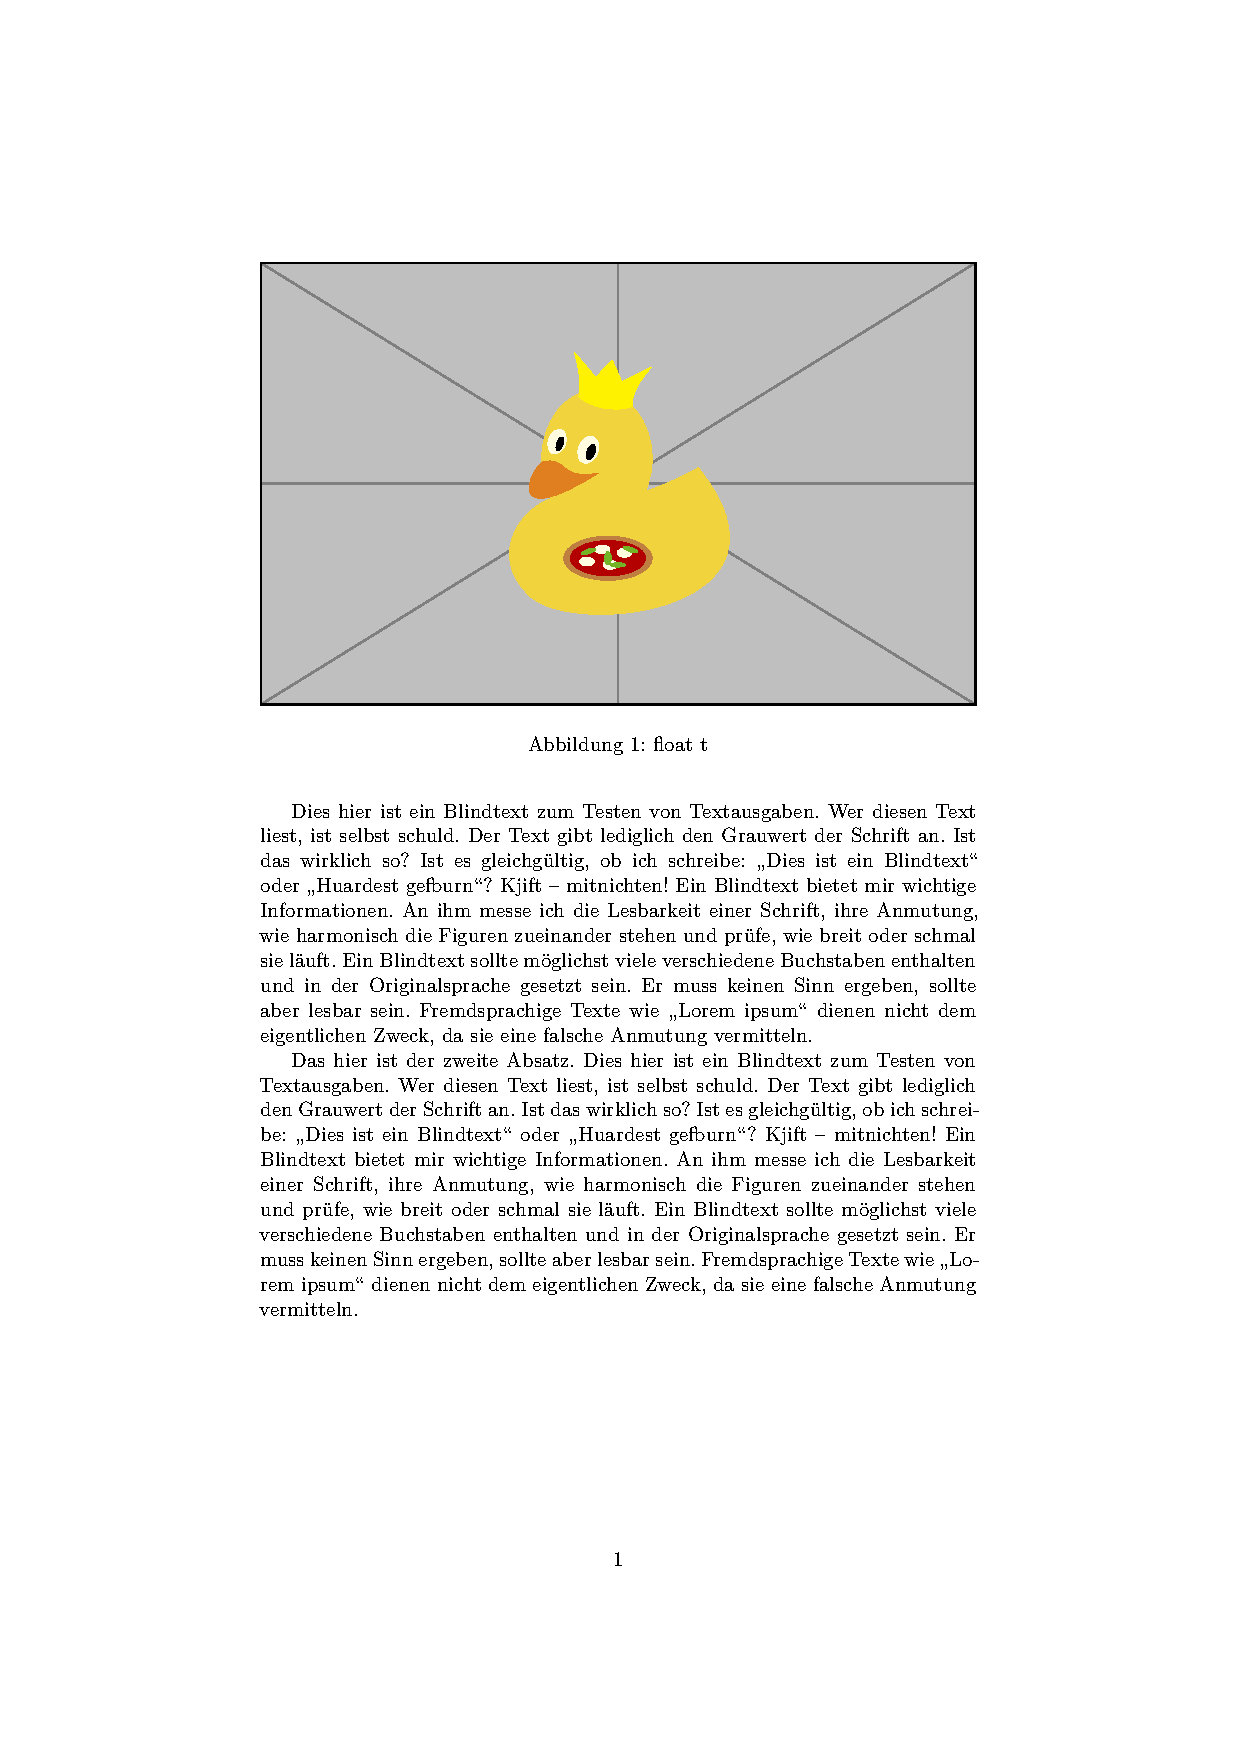
\includegraphics[page=1,width=\linewidth]{images/float/float.pdf}
            \raisebox{5ex}{\invisirule{}}
        \end{subfigure}%
        \begin{subfigure}{.3333\textwidth}
            \centering
            \includegraphics[page=2,width=\linewidth]{images/float/float.pdf}
            \raisebox{5ex}{\wrongrule{}}
        \end{subfigure}%
        \begin{subfigure}{.3333\textwidth}
            \centering
            \includegraphics[page=3,width=\linewidth]{images/float/float.pdf}
            \raisebox{5ex}{\invisirule{}}
        \end{subfigure}%
    \end{figure}
\end{frame}

\begin{frame}[fragile]
    \frametitle{Schusterjungen und Hurenkinder}
    \begin{figure}
        \centering%
        \begin{subfigure}{.35\textwidth}
            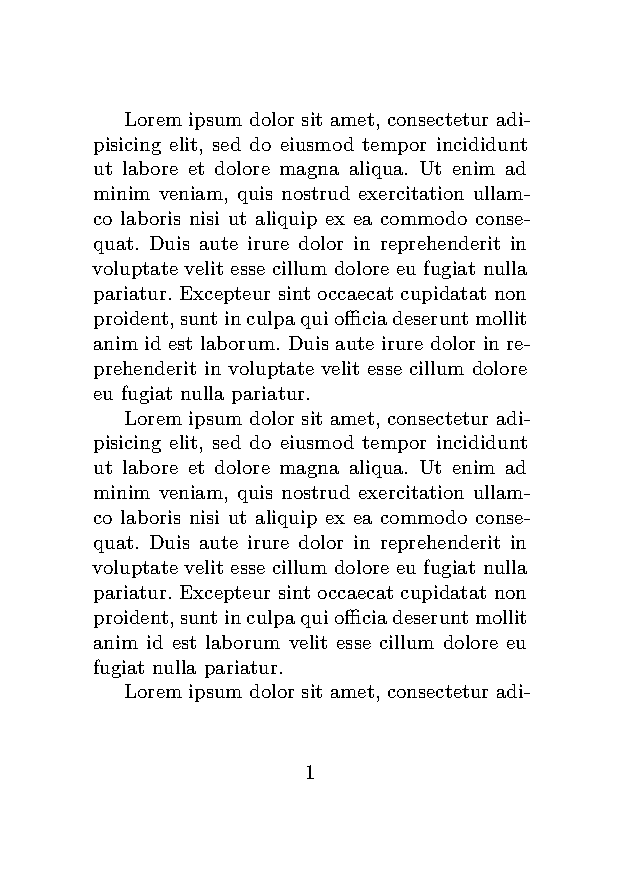
\includegraphics[page=1,width=\linewidth]{images/hurenkind/hurenkind.pdf}
        \end{subfigure}%
        \begin{subfigure}{.35\textwidth}
            \includegraphics[page=2,width=\linewidth]{images/hurenkind/hurenkind.pdf}
        \end{subfigure}%
    \end{figure}
    \pause

    \begin{lstlisting}
\widowpenalty10000 % Preamble
\clubpenalty10000 % Preamble
    \end{lstlisting}

    \begin{lstlisting}
\usepackage[all]{nowidow} % Preamble
    \end{lstlisting}
    \note[item]{Schusterjunge = Orphan}
\end{frame}

\begin{frame}[fragile]
    \frametitle{Smallcaps, Oldstyle}%
    \vspace*{-2.5ex}
    \begin{multicols}{2}
        \small\justifying
        Die NASA (National Aeronautics and Space Administration) ist die $1958$ gegründete zivile US-Bundesbehörde für Raumfahrt und Flugwissenschaft.
        Der Hauptsitz befindet sich in Washington, DC.
        Zugleich ist die NASA eine wichtige geowissenschaftliche Forschungsinstitution und stellt in den USA die meisten Forschungsgelder für klimawissenschaftliche Forschungsarbeiten bereit.

        ~~~~~Im Februar $2006$ strich die NASA den Schutz der Erde aus ihrem mission statement, um es dem von George W. Bush verkündeten Raumflugprogramm anzugleichen.

        Die \textsc{nasa} (National Aeronautics and Space Administration) ist die 1958 gegründete zivile \textsc{us}-Bundesbehörde für Raumfahrt und Flugwissenschaft.
        Der Hauptsitz befindet sich in Washington, \textsc{dc}.
        Zugleich ist die \textsc{nasa} eine wichtige geowissenschaftliche Forschungsinstitution und stellt in den \textsc{usa} die meisten Forschungsgelder für klimawissenschaftliche Forschungsarbeiten bereit.

        ~~~~~Im Februar 2006 strich die \textsc{nasa} den Schutz der Erde aus ihrem mission statement, um es dem von George W. Bush verkündeten Raumflugprogramm anzugleichen.
    \end{multicols}
    \pause
    Kein wissenschaftliches Style Manual will das aber tatsächlich!
    \note[item]{Kapitälchen}
    \note[item]{Mediävalziffern}
    \note[item]{Nicht bei W.}
\end{frame}

% == == == == == == == == == == == == == == == == == == == == == == == == == == == ==
\section{Paketempfehlungen}

\sectiontitlepage

\begin{frame}[fragile]
    \frametitle{tikzplotlib -- Python Matplotlib als TikZ export}%
    \vspace*{-1ex}
    \begin{figure}
        \begin{subfigure}{0.5\textwidth}
            \centering
            \raisebox{6ex}{
\includegraphics[width=.4\linewidth]{images/python}}
        \end{subfigure}%
        \begin{subfigure}{0.5\textwidth}
            \centering
            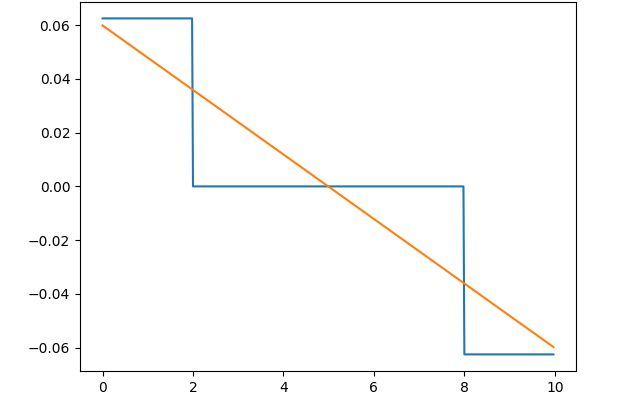
\includegraphics[width=.8\linewidth]{images/tikzplotlib/tpl-example-crop}
            \caption{Matplotlib}
        \end{subfigure}%

        \begin{subfigure}{0.5\textwidth}
            % This file was created with tikzplotlib v0.10.1.
\begin{tikzpicture}

\definecolor{darkgray176}{RGB}{176,176,176}
\definecolor{darkorange25512714}{RGB}{255,127,14}
\definecolor{steelblue31119180}{RGB}{31,119,180}

\begin{axis}[
tick align=outside,
tick pos=left,
            width=\linewidth,
            height=.45\paperheight,
x grid style={darkgray176},
xmin=-0.4985, xmax=10.4685,
xtick style={color=black},
y grid style={darkgray176},
ymin=-0.0687500000033578, ymax=0.0687500000004435,
ytick style={color=black}
]
\addplot [semithick, steelblue31119180]
table {%
0 0.0625
0.01 0.0625
0.02 0.0625
0.03 0.0625000000000001
0.04 0.0624999999999997
0.05 0.0625000000000004
0.06 0.0624999999999996
0.07 0.0624999999999999
0.08 0.0625000000000009
0.09 0.0624999999999986
0.1 0.0625000000000007
0.11 0.0625000000000007
0.12 0.0624999999999995
0.13 0.0624999999999987
0.14 0.0625000000000018
0.15 0.0625000000000006
0.16 0.0624999999999964
0.17 0.0625000000000028
0.18 0.0625000000000018
0.19 0.0624999999999931
0.2 0.0625000000000061
0.21 0.0624999999999997
0.22 0.0624999999999975
0.23 0.0625000000000018
0.24 0.0625000000000016
0.25 0.0624999999999976
0.26 0.0625000000000018
0.27 0.0624999999999931
0.28 0.062500000000006
0.29 0.0625000000000018
0.3 0.0624999999999976
0.31 0.0625000000000018
0.32 0.0625000000000018
0.33 0.0624999999999973
0.34 0.062499999999989
0.35 0.0625000000000105
0.36 0.0625000000000018
0.37 0.0625000000000018
0.38 0.0625000000000018
0.39 0.0624999999999931
0.4 0.0624999999999844
0.41 0.0625000000000191
0.42 0.0625000000000018
0.43 0.0625000000000018
0.44 0.0624999999999931
0.45 0.0625000000000105
0.46 0.0624999999999758
0.47 0.0625000000000105
0.48 0.0625000000000105
0.49 0.0624999999999931
0.5 0.0625000000000105
0.51 0.0624999999999931
0.52 0.0624999999999931
0.53 0.0625000000000105
0.54 0.0624999999999931
0.55 0.0625000000000105
0.56 0.0624999999999584
0.57 0.0625000000000278
0.58 0.0625000000000105
0.59 0.0624999999999931
0.6 0.0625000000000105
0.61 0.0624999999999931
0.62 0.0624999999999931
0.63 0.0625000000000105
0.64 0.0624999999999931
0.65 0.0625000000000105
0.66 0.0624999999999931
0.67 0.0624999999999931
0.68 0.0625000000000105
0.69 0.0624999999999584
0.7 0.0625000000000278
0.71 0.0624999999999931
0.72 0.0625000000000278
0.73 0.0624999999999931
0.74 0.0624999999999931
0.75 0.0624999999999931
0.76 0.0625000000000278
0.77 0.0624999999999931
0.78 0.0624999999999931
0.79 0.0624999999999931
0.8 0.0624999999999931
0.81 0.0624999999999931
0.82 0.0624999999999584
0.83 0.0625000000000625
0.84 0.0624999999999931
0.85 0.0625000000000278
0.86 0.0624999999999584
0.87 0.0625000000000278
0.88 0.0624999999999931
0.89 0.0624999999999931
0.9 0.0624999999999931
0.91 0.0625000000000278
0.92 0.0624999999999931
0.93 0.0624999999999584
0.94 0.0624999999999931
0.95 0.0625000000000278
0.96 0.0624999999999931
0.97 0.0625000000000278
0.98 0.0624999999999931
0.99 0.0624999999999931
1 0.0624999999999931
1.01 0.0624999999999931
1.02 0.0625000000000625
1.03 0.0624999999999237
1.04 0.0625000000000625
1.05 0.0624999999999237
1.06 0.0625000000000625
1.07 0.0624999999999931
1.08 0.0624999999999931
1.09 0.0624999999999931
1.1 0.0624999999999931
1.11 0.0625000000000625
1.12 0.0624999999999237
1.13 0.0624999999999931
1.14 0.0624999999999237
1.15 0.0625000000000625
1.16 0.0625000000000625
1.17 0.0624999999999931
1.18 0.0624999999999931
1.19 0.0624999999999931
1.2 0.0624999999999931
1.21 0.0624999999999931
1.22 0.0625000000000625
1.23 0.0624999999999237
1.24 0.0625000000000625
1.25 0.0624999999999237
1.26 0.0625000000000625
1.27 0.0624999999999931
1.28 0.0624999999999931
1.29 0.0624999999999931
1.3 0.0624999999999931
1.31 0.0624999999999931
1.32 0.0625000000000625
1.33 0.0624999999999237
1.34 0.0625000000000625
1.35 0.0624999999999237
1.36 0.0625000000000625
1.37 0.0624999999999931
1.38 0.0624999999999931
1.39 0.0624999999997849
1.4 0.0625000000002707
1.41 0.0624999999998543
1.42 0.0625000000001319
1.43 0.0624999999999931
1.44 0.0624999999998543
1.45 0.0625000000001319
1.46 0.0624999999999931
1.47 0.0624999999999931
1.48 0.0624999999999931
1.49 0.0624999999999931
1.5 0.0624999999999931
1.51 0.0624999999999931
1.52 0.0624999999999931
1.53 0.0625000000001319
1.54 0.0624999999998543
1.55 0.0624999999999931
1.56 0.0625000000001319
1.57 0.0624999999998543
1.58 0.0625000000001319
1.59 0.0624999999998543
1.6 0.0625000000001319
1.61 0.0624999999998543
1.62 0.0625000000001319
1.63 0.0624999999999931
1.64 0.0624999999998543
1.65 0.0624999999999931
1.66 0.0624999999999931
1.67 0.0625000000001319
1.68 0.0624999999999931
1.69 0.0624999999999931
1.7 0.0624999999999931
1.71 0.0625000000001319
1.72 0.0624999999998543
1.73 0.0624999999999931
1.74 0.0624999999999931
1.75 0.0625000000001319
1.76 0.0624999999998543
1.77 0.0624999999999931
1.78 0.0625000000001319
1.79 0.0624999999998543
1.8 0.0625000000001319
1.81 0.0624999999999931
1.82 0.0624999999998543
1.83 0.0625000000001319
1.84 0.0624999999999931
1.85 0.0624999999999931
1.86 0.0624999999999931
1.87 0.0624999999998543
1.88 0.0625000000001319
1.89 0.0624999999999931
1.9 0.0624999999998543
1.91 0.0625000000001319
1.92 0.0624999999999931
1.93 0.0624999999999931
1.94 0.0624999999999931
1.95 0.0625000000001319
1.96 0.0624999999998543
1.97 0.0625000000001319
1.98 0.0624999999998543
1.99 0.0312500000003435
2 -5.55111512312578e-13
2.01 5.55111512312578e-13
2.02 -5.55111512312578e-13
2.03 0
2.04 5.55111512312578e-13
2.05 -5.55111512312578e-13
2.06 5.55111512312578e-13
2.07 -5.55111512312578e-13
2.08 5.55111512312578e-13
2.09 -5.55111512312578e-13
2.1 5.55111512312578e-13
2.11 -5.55111512312578e-13
2.12 5.55111512312578e-13
2.13 -5.55111512312578e-13
2.14 5.55111512312578e-13
2.15 -5.55111512312578e-13
2.16 5.55111512312578e-13
2.17 -5.55111512312578e-13
2.18 5.55111512312578e-13
2.19 -5.55111512312578e-13
2.2 5.55111512312578e-13
2.21 -5.55111512312578e-13
2.22 5.55111512312578e-13
2.23 -5.55111512312578e-13
2.24 5.55111512312578e-13
2.25 -5.55111512312578e-13
2.26 5.55111512312578e-13
2.27 -5.55111512312578e-13
2.28 5.55111512312578e-13
2.29 -5.55111512312578e-13
2.3 0
2.31 5.55111512312578e-13
2.32 -5.55111512312578e-13
2.33 5.55111512312578e-13
2.34 -5.55111512312578e-13
2.35 5.55111512312578e-13
2.36 -5.55111512312578e-13
2.37 5.55111512312578e-13
2.38 -5.55111512312578e-13
2.39 5.55111512312578e-13
2.4 -5.55111512312578e-13
2.41 5.55111512312578e-13
2.42 -5.55111512312578e-13
2.43 5.55111512312578e-13
2.44 -5.55111512312578e-13
2.45 5.55111512312578e-13
2.46 -5.55111512312578e-13
2.47 5.55111512312578e-13
2.48 -5.55111512312578e-13
2.49 5.55111512312578e-13
2.5 -5.55111512312578e-13
2.51 5.55111512312578e-13
2.52 -5.55111512312578e-13
2.53 5.55111512312578e-13
2.54 -5.55111512312578e-13
2.55 0
2.56 5.55111512312578e-13
2.57 -5.55111512312578e-13
2.58 5.55111512312578e-13
2.59 -5.55111512312578e-13
2.6 5.55111512312578e-13
2.61 -5.55111512312578e-13
2.62 5.55111512312578e-13
2.63 -5.55111512312578e-13
2.64 5.55111512312578e-13
2.65 -5.55111512312578e-13
2.66 5.55111512312578e-13
2.67 -5.55111512312578e-13
2.68 5.55111512312578e-13
2.69 -5.55111512312578e-13
2.7 5.55111512312578e-13
2.71 -5.55111512312578e-13
2.72 5.55111512312578e-13
2.73 -5.55111512312578e-13
2.74 5.55111512312578e-13
2.75 -5.55111512312578e-13
2.76 5.55111512312578e-13
2.77 -5.55111512312578e-13
2.78 5.55111512312578e-13
2.79 -5.55111512312578e-13
2.8 0
2.81 5.55111512312578e-13
2.82 -5.55111512312578e-13
2.83 5.55111512312578e-13
2.84 -5.55111512312578e-13
2.85 5.55111512312578e-13
2.86 -5.55111512312578e-13
2.87 5.55111512312578e-13
2.88 -5.55111512312578e-13
2.89 5.55111512312578e-13
2.9 -5.55111512312578e-13
2.91 5.55111512312578e-13
2.92 -5.55111512312578e-13
2.93 5.55111512312578e-13
2.94 -5.55111512312578e-13
2.95 5.55111512312578e-13
2.96 -5.55111512312578e-13
2.97 5.55111512312578e-13
2.98 -5.55111512312578e-13
2.99 5.55111512312578e-13
3 -5.55111512312578e-13
3.01 5.55111512312578e-13
3.02 -5.55111512312578e-13
3.03 5.55111512312578e-13
3.04 -5.55111512312578e-13
3.05 5.55111512312578e-13
3.06 -5.55111512312578e-13
3.07 0
3.08 5.55111512312578e-13
3.09 -5.55111512312578e-13
3.1 5.55111512312578e-13
3.11 -5.55111512312578e-13
3.12 5.55111512312578e-13
3.13 -5.55111512312578e-13
3.14 5.55111512312578e-13
3.15 -5.55111512312578e-13
3.16 5.55111512312578e-13
3.17 -5.55111512312578e-13
3.18 5.55111512312578e-13
3.19 -5.55111512312578e-13
3.2 5.55111512312578e-13
3.21 -5.55111512312578e-13
3.22 5.55111512312578e-13
3.23 -5.55111512312578e-13
3.24 5.55111512312578e-13
3.25 -5.55111512312578e-13
3.26 5.55111512312578e-13
3.27 -5.55111512312578e-13
3.28 5.55111512312578e-13
3.29 -5.55111512312578e-13
3.3 5.55111512312578e-13
3.31 -5.55111512312578e-13
3.32 0
3.33 5.55111512312578e-13
3.34 -5.55111512312578e-13
3.35 5.55111512312578e-13
3.36 -5.55111512312578e-13
3.37 5.55111512312578e-13
3.38 -5.55111512312578e-13
3.39 5.55111512312578e-13
3.4 -5.55111512312578e-13
3.41 5.55111512312578e-13
3.42 -5.55111512312578e-13
3.43 5.55111512312578e-13
3.44 -5.55111512312578e-13
3.45 5.55111512312578e-13
3.46 -5.55111512312578e-13
3.47 5.55111512312578e-13
3.48 -5.55111512312578e-13
3.49 5.55111512312578e-13
3.5 -5.55111512312578e-13
3.51 5.55111512312578e-13
3.52 -5.55111512312578e-13
3.53 5.55111512312578e-13
3.54 -5.55111512312578e-13
3.55 5.55111512312578e-13
3.56 -5.55111512312578e-13
3.57 0
3.58 5.55111512312578e-13
3.59 -5.55111512312578e-13
3.6 5.55111512312578e-13
3.61 -5.55111512312578e-13
3.62 5.55111512312578e-13
3.63 -5.55111512312578e-13
3.64 5.55111512312578e-13
3.65 -5.55111512312578e-13
3.66 5.55111512312578e-13
3.67 -5.55111512312578e-13
3.68 5.55111512312578e-13
3.69 -5.55111512312578e-13
3.7 5.55111512312578e-13
3.71 -5.55111512312578e-13
3.72 5.55111512312578e-13
3.73 -5.55111512312578e-13
3.74 5.55111512312578e-13
3.75 -5.55111512312578e-13
3.76 5.55111512312578e-13
3.77 -5.55111512312578e-13
3.78 5.55111512312578e-13
3.79 -5.55111512312578e-13
3.8 5.55111512312578e-13
3.81 -5.55111512312578e-13
3.82 0
3.83 5.55111512312578e-13
3.84 -5.55111512312578e-13
3.85 5.55111512312578e-13
3.86 -5.55111512312578e-13
3.87 5.55111512312578e-13
3.88 -5.55111512312578e-13
3.89 5.55111512312578e-13
3.9 -5.55111512312578e-13
3.91 5.55111512312578e-13
3.92 -5.55111512312578e-13
3.93 5.55111512312578e-13
3.94 -5.55111512312578e-13
3.95 5.55111512312578e-13
3.96 -5.55111512312578e-13
3.97 5.55111512312578e-13
3.98 -5.55111512312578e-13
3.99 0
4 1.11022302462516e-12
4.01 -1.11022302462516e-12
4.02 0
4.03 0
4.04 1.11022302462516e-12
4.05 -1.11022302462516e-12
4.06 0
4.07 0
4.08 0
4.09 1.11022302462516e-12
4.1 -1.11022302462516e-12
4.11 0
4.12 0
4.13 1.11022302462516e-12
4.14 -1.11022302462516e-12
4.15 0
4.16 0
4.17 1.11022302462516e-12
4.18 -1.11022302462516e-12
4.19 0
4.2 0
4.21 1.11022302462516e-12
4.22 -1.11022302462516e-12
4.23 0
4.24 0
4.25 1.11022302462516e-12
4.26 -1.11022302462516e-12
4.27 0
4.28 0
4.29 1.11022302462516e-12
4.3 -1.11022302462516e-12
4.31 0
4.32 0
4.33 1.11022302462516e-12
4.34 -1.11022302462516e-12
4.35 0
4.36 0
4.37 0
4.38 1.11022302462516e-12
4.39 -1.11022302462516e-12
4.4 0
4.41 0
4.42 1.11022302462516e-12
4.43 -1.11022302462516e-12
4.44 0
4.45 0
4.46 1.11022302462516e-12
4.47 -1.11022302462516e-12
4.48 0
4.49 0
4.5 1.11022302462516e-12
4.51 -1.11022302462516e-12
4.52 0
4.53 0
4.54 1.11022302462516e-12
4.55 -1.11022302462516e-12
4.56 0
4.57 0
4.58 1.11022302462516e-12
4.59 -1.11022302462516e-12
4.6 0
4.61 0
4.62 0
4.63 1.11022302462516e-12
4.64 -1.11022302462516e-12
4.65 0
4.66 0
4.67 1.11022302462516e-12
4.68 -1.11022302462516e-12
4.69 0
4.7 0
4.71 1.11022302462516e-12
4.72 -1.11022302462516e-12
4.73 0
4.74 0
4.75 1.11022302462516e-12
4.76 -1.11022302462516e-12
4.77 0
4.78 0
4.79 1.11022302462516e-12
4.8 -1.11022302462516e-12
4.81 0
4.82 0
4.83 1.11022302462516e-12
4.84 -1.11022302462516e-12
4.85 0
4.86 0
4.87 0
4.88 1.11022302462516e-12
4.89 -1.11022302462516e-12
4.9 0
4.91 0
4.92 1.11022302462516e-12
4.93 -1.11022302462516e-12
4.94 0
4.95 0
4.96 1.11022302462516e-12
4.97 -1.11022302462516e-12
4.98 0
4.99 0
5 1.11022302462516e-12
5.01 -1.11022302462516e-12
5.02 0
5.03 0
5.04 1.11022302462516e-12
5.05 -1.11022302462516e-12
5.06 0
5.07 0
5.08 1.11022302462516e-12
5.09 -1.11022302462516e-12
5.1 0
5.11 0
5.12 0
5.13 1.11022302462516e-12
5.14 -1.11022302462516e-12
5.15 0
5.16 0
5.17 1.11022302462516e-12
5.18 -1.11022302462516e-12
5.19 0
5.2 0
5.21 1.11022302462516e-12
5.22 -1.11022302462516e-12
5.23 0
5.24 0
5.25 1.11022302462516e-12
5.26 -1.11022302462516e-12
5.27 0
5.28 0
5.29 1.11022302462516e-12
5.3 -1.11022302462516e-12
5.31 0
5.32 0
5.33 1.11022302462516e-12
5.34 -1.11022302462516e-12
5.35 0
5.36 0
5.37 0
5.38 1.11022302462516e-12
5.39 -1.11022302462516e-12
5.4 0
5.41 0
5.42 1.11022302462516e-12
5.43 -1.11022302462516e-12
5.44 0
5.45 0
5.46 1.11022302462516e-12
5.47 -1.11022302462516e-12
5.48 0
5.49 0
5.5 1.11022302462516e-12
5.51 -1.11022302462516e-12
5.52 0
5.53 0
5.54 1.11022302462516e-12
5.55 -1.11022302462516e-12
5.56 0
5.57 0
5.58 1.11022302462516e-12
5.59 -1.11022302462516e-12
5.6 0
5.61 0
5.62 0
5.63 1.11022302462516e-12
5.64 -1.11022302462516e-12
5.65 0
5.66 0
5.67 1.11022302462516e-12
5.68 -1.11022302462516e-12
5.69 0
5.7 0
5.71 1.11022302462516e-12
5.72 -1.11022302462516e-12
5.73 0
5.74 0
5.75 1.11022302462516e-12
5.76 -1.11022302462516e-12
5.77 0
5.78 0
5.79 1.11022302462516e-12
5.8 -1.11022302462516e-12
5.81 0
5.82 0
5.83 1.11022302462516e-12
5.84 -1.11022302462516e-12
5.85 0
5.86 0
5.87 0
5.88 1.11022302462516e-12
5.89 -1.11022302462516e-12
5.9 0
5.91 0
5.92 1.11022302462516e-12
5.93 -1.11022302462516e-12
5.94 0
5.95 0
5.96 1.11022302462516e-12
5.97 -1.11022302462516e-12
5.98 0
5.99 0
6 1.11022302462516e-12
6.01 -1.11022302462516e-12
6.02 0
6.03 0
6.04 1.11022302462516e-12
6.05 -1.11022302462516e-12
6.06 0
6.07 0
6.08 1.11022302462516e-12
6.09 -1.11022302462516e-12
6.1 0
6.11 0
6.12 1.11022302462516e-12
6.13 -1.11022302462516e-12
6.14 0
6.15 0
6.16 0
6.17 1.11022302462516e-12
6.18 -1.11022302462516e-12
6.19 0
6.2 0
6.21 1.11022302462516e-12
6.22 -1.11022302462516e-12
6.23 0
6.24 0
6.25 1.11022302462516e-12
6.26 -1.11022302462516e-12
6.27 0
6.28 0
6.29 1.11022302462516e-12
6.3 -1.11022302462516e-12
6.31 0
6.32 0
6.33 1.11022302462516e-12
6.34 -1.11022302462516e-12
6.35 0
6.36 0
6.37 1.11022302462516e-12
6.38 -1.11022302462516e-12
6.39 0
6.4 0
6.41 0
6.42 1.11022302462516e-12
6.43 -1.11022302462516e-12
6.44 0
6.45 0
6.46 1.11022302462516e-12
6.47 -1.11022302462516e-12
6.48 0
6.49 0
6.5 1.11022302462516e-12
6.51 -1.11022302462516e-12
6.52 0
6.53 0
6.54 1.11022302462516e-12
6.55 -1.11022302462516e-12
6.56 0
6.57 0
6.58 1.11022302462516e-12
6.59 -1.11022302462516e-12
6.6 0
6.61 0
6.62 1.11022302462516e-12
6.63 -1.11022302462516e-12
6.64 0
6.65 0
6.66 0
6.67 1.11022302462516e-12
6.68 -1.11022302462516e-12
6.69 0
6.7 0
6.71 1.11022302462516e-12
6.72 -1.11022302462516e-12
6.73 0
6.74 0
6.75 1.11022302462516e-12
6.76 -1.11022302462516e-12
6.77 0
6.78 0
6.79 1.11022302462516e-12
6.8 -1.11022302462516e-12
6.81 0
6.82 0
6.83 1.11022302462516e-12
6.84 -1.11022302462516e-12
6.85 0
6.86 0
6.87 1.11022302462516e-12
6.88 -1.11022302462516e-12
6.89 0
6.9 0
6.91 0
6.92 1.11022302462516e-12
6.93 -1.11022302462516e-12
6.94 0
6.95 0
6.96 1.11022302462516e-12
6.97 -1.11022302462516e-12
6.98 0
6.99 0
7 1.11022302462516e-12
7.01 -1.11022302462516e-12
7.02 0
7.03 0
7.04 1.11022302462516e-12
7.05 -1.11022302462516e-12
7.06 0
7.07 0
7.08 1.11022302462516e-12
7.09 -1.11022302462516e-12
7.1 0
7.11 0
7.12 1.11022302462516e-12
7.13 -1.11022302462516e-12
7.14 0
7.15 0
7.16 0
7.17 1.11022302462516e-12
7.18 -1.11022302462516e-12
7.19 0
7.2 0
7.21 1.11022302462516e-12
7.22 -1.11022302462516e-12
7.23 0
7.24 0
7.25 1.11022302462516e-12
7.26 -1.11022302462516e-12
7.27 0
7.28 0
7.29 1.11022302462516e-12
7.3 -1.11022302462516e-12
7.31 0
7.32 0
7.33 1.11022302462516e-12
7.34 -1.11022302462516e-12
7.35 0
7.36 0
7.37 1.11022302462516e-12
7.38 -1.11022302462516e-12
7.39 0
7.4 0
7.41 0
7.42 1.11022302462516e-12
7.43 -1.11022302462516e-12
7.44 0
7.45 0
7.46 1.11022302462516e-12
7.47 -1.11022302462516e-12
7.48 0
7.49 0
7.5 1.11022302462516e-12
7.51 -1.11022302462516e-12
7.52 0
7.53 0
7.54 1.11022302462516e-12
7.55 -1.11022302462516e-12
7.56 0
7.57 0
7.58 1.11022302462516e-12
7.59 -1.11022302462516e-12
7.6 0
7.61 0
7.62 1.11022302462516e-12
7.63 -1.11022302462516e-12
7.64 0
7.65 0
7.66 0
7.67 1.11022302462516e-12
7.68 -1.11022302462516e-12
7.69 0
7.7 0
7.71 1.11022302462516e-12
7.72 -1.11022302462516e-12
7.73 0
7.74 0
7.75 1.11022302462516e-12
7.76 -1.11022302462516e-12
7.77 0
7.78 0
7.79 1.11022302462516e-12
7.8 -1.11022302462516e-12
7.81 0
7.82 0
7.83 1.11022302462516e-12
7.84 -1.11022302462516e-12
7.85 0
7.86 0
7.87 1.11022302462516e-12
7.88 -1.11022302462516e-12
7.89 0
7.9 0
7.91 1.11022302462516e-12
7.92 -1.11022302462516e-12
7.93 0
7.94 0
7.95 0
7.96 1.11022302462516e-12
7.97 -1.11022302462516e-12
7.98 0
7.99 -0.0312499999999272
8 -0.0624999999998543
8.01 -0.0625000000009646
8.02 -0.0624999999965237
8.03 -0.062500000003185
8.04 -0.0624999999987441
8.05 -0.0625000000009646
8.06 -0.0624999999998543
8.07 -0.0624999999998543
8.08 -0.0624999999998543
8.09 -0.0625000000009646
8.1 -0.0624999999976339
8.11 -0.0625000000009646
8.12 -0.0625000000009646
8.13 -0.0624999999998543
8.14 -0.0624999999998543
8.15 -0.0624999999998543
8.16 -0.0624999999998543
8.17 -0.0625000000009646
8.18 -0.0624999999987441
8.19 -0.0624999999987441
8.2 -0.0625000000020748
8.21 -0.0624999999998543
8.22 -0.0624999999998543
8.23 -0.0624999999998543
8.24 -0.0624999999998543
8.25 -0.0625000000009646
8.26 -0.0624999999987441
8.27 -0.0624999999987441
8.28 -0.0625000000020748
8.29 -0.0624999999998543
8.3 -0.0624999999998543
8.31 -0.0624999999998543
8.32 -0.0625000000009646
8.33 -0.0624999999987441
8.34 -0.0625000000009646
8.35 -0.0624999999976339
8.36 -0.0625000000020748
8.37 -0.0624999999998543
8.38 -0.0624999999998543
8.39 -0.0624999999998543
8.4 -0.0625000000009646
8.41 -0.0624999999987441
8.42 -0.0625000000009646
8.43 -0.0624999999998543
8.44 -0.0624999999976339
8.45 -0.0625000000020748
8.46 -0.0624999999998543
8.47 -0.0625000000009646
8.48 -0.0624999999987441
8.49 -0.0625000000009646
8.5 -0.0624999999987441
8.51 -0.0625000000009646
8.52 -0.0624999999987441
8.53 -0.0625000000009646
8.54 -0.0624999999998543
8.55 -0.0624999999998543
8.56 -0.0625000000009646
8.57 -0.0624999999987441
8.58 -0.0625000000009646
8.59 -0.0624999999998543
8.6 -0.0624999999976339
8.61 -0.062500000003185
8.62 -0.0624999999987441
8.63 -0.0624999999998543
8.64 -0.0625000000009646
8.65 -0.0624999999987441
8.66 -0.0625000000009646
8.67 -0.0624999999998543
8.68 -0.0624999999987441
8.69 -0.0625000000009646
8.7 -0.0624999999998543
8.71 -0.0625000000009646
8.72 -0.0624999999987441
8.73 -0.0625000000009646
8.74 -0.0624999999998543
8.75 -0.0624999999998543
8.76 -0.0624999999998543
8.77 -0.0624999999987441
8.78 -0.0625000000009646
8.79 -0.0625000000009646
8.8 -0.0624999999987441
8.81 -0.0625000000009646
8.82 -0.0624999999998543
8.83 -0.0624999999998543
8.84 -0.0624999999998543
8.85 -0.0624999999987441
8.86 -0.0625000000009646
8.87 -0.0625000000009646
8.88 -0.0624999999998543
8.89 -0.0624999999987441
8.9 -0.0625000000009646
8.91 -0.0624999999998543
8.92 -0.0624999999998543
8.93 -0.0624999999998543
8.94 -0.0624999999998543
8.95 -0.0625000000009646
8.96 -0.0624999999987441
8.97 -0.0625000000009646
8.98 -0.0624999999998543
8.99 -0.0624999999998543
9 -0.0624999999998543
9.01 -0.0625000000009646
9.02 -0.0624999999976339
9.03 -0.0625000000020748
9.04 -0.0624999999987441
9.05 -0.0625000000009646
9.06 -0.0624999999998543
9.07 -0.0624999999998543
9.08 -0.0625000000009646
9.09 -0.0624999999987441
9.1 -0.0624999999998543
9.11 -0.0624999999998543
9.12 -0.0625000000009646
9.13 -0.0624999999998543
9.14 -0.0624999999998543
9.15 -0.0624999999998543
9.16 -0.0624999999998543
9.17 -0.0625000000009646
9.18 -0.0624999999976339
9.19 -0.0625000000020748
9.2 -0.0624999999998543
9.21 -0.0624999999998543
9.22 -0.0624999999998543
9.23 -0.0624999999998543
9.24 -0.0624999999998543
9.25 -0.0625000000009646
9.26 -0.0624999999987441
9.27 -0.0624999999998543
9.28 -0.0625000000009646
9.29 -0.0624999999998543
9.3 -0.0624999999998543
9.31 -0.0624999999998543
9.32 -0.0625000000009646
9.33 -0.0624999999987441
9.34 -0.0625000000009646
9.35 -0.0624999999987441
9.36 -0.0625000000009646
9.37 -0.0624999999998543
9.38 -0.0624999999998543
9.39 -0.0624999999998543
9.4 -0.0625000000009646
9.41 -0.0624999999987441
9.42 -0.0625000000009646
9.43 -0.0624999999987441
9.44 -0.0625000000009646
9.45 -0.0624999999998543
9.46 -0.0624999999998543
9.47 -0.0625000000009646
9.48 -0.0624999999987441
9.49 -0.0625000000009646
9.5 -0.0624999999987441
9.51 -0.0625000000009646
9.52 -0.0624999999998543
9.53 -0.0624999999998543
9.54 -0.0624999999998543
9.55 -0.0624999999998543
9.56 -0.0625000000009646
9.57 -0.0624999999987441
9.58 -0.0625000000009646
9.59 -0.0624999999998543
9.6 -0.0624999999998543
9.61 -0.0624999999998543
9.62 -0.0624999999998543
9.63 -0.0624999999998543
9.64 -0.0625000000009646
9.65 -0.0624999999987441
9.66 -0.0625000000009646
9.67 -0.0624999999998543
9.68 -0.0624999999998543
9.69 -0.0624999999998543
9.7 -0.0624999999998543
9.71 -0.0625000000009646
9.72 -0.0624999999987441
9.73 -0.0625000000009646
9.74 -0.0624999999998543
9.75 -0.0624999999998543
9.76 -0.0624999999998543
9.77 -0.0624999999998543
9.78 -0.0624999999998543
9.79 -0.0625000000009646
9.8 -0.0624999999987441
9.81 -0.0625000000009646
9.82 -0.0624999999998543
9.83 -0.0624999999998543
9.84 -0.0624999999998543
9.85 -0.0624999999998543
9.86 -0.0624999999998543
9.87 -0.0625000000009646
9.88 -0.0624999999998543
9.89 -0.0624999999987441
9.9 -0.0625000000009646
9.91 -0.0624999999998543
9.92 -0.0624999999998543
9.93 -0.0625000000009646
9.94 -0.0624999999987441
9.95 -0.0625000000009646
9.96 -0.0624999999987441
9.97 -0.0625000000009646
};
\addplot [semithick, darkorange25512714]
table {%
0 0.05988
0.01 0.05976
0.02 0.05964
0.03 0.05952
0.04 0.0593999999999999
0.05 0.0592800000000001
0.06 0.0591599999999999
0.07 0.0590399999999996
0.08 0.058920000000001
0.09 0.0587999999999988
0.1 0.0586800000000007
0.11 0.0585600000000005
0.12 0.0584399999999996
0.13 0.0583199999999978
0.14 0.0582000000000036
0.15 0.0580799999999994
0.16 0.0579599999999963
0.17 0.0578400000000033
0.18 0.0577200000000014
0.19 0.0575999999999939
0.2 0.0574800000000052
0.21 0.0573600000000011
0.22 0.0572399999999969
0.23 0.0571199999999996
0.24 0.0570000000000041
0.25 0.0568799999999979
0.26 0.0567600000000003
0.27 0.0566399999999898
0.28 0.0565200000000137
0.29 0.0563999999999992
0.3 0.0562799999999926
0.31 0.0561600000000082
0.32 0.0560399999999978
0.33 0.0559199999999999
0.34 0.0557999999999854
0.35 0.0556800000000135
0.36 0.0555599999999989
0.37 0.0554400000000056
0.38 0.0553199999999993
0.39 0.0551999999999931
0.4 0.0550799999999869
0.41 0.0549600000000153
0.42 0.0548400000000091
0.43 0.0547199999999942
0.44 0.0545999999999967
0.45 0.0544800000000078
0.46 0.0543599999999755
0.47 0.0542400000000127
0.48 0.0541200000000065
0.49 0.0540000000000002
0.5 0.0538800000000027
0.51 0.0537599999999878
0.52 0.0536400000000076
0.53 0.0535200000000187
0.54 0.0533999999999778
0.55 0.0532800000000062
0.56 0.0531599999999653
0.57 0.0530400000000285
0.58 0.0529200000000049
0.59 0.0527999999999987
0.6 0.0526800000000098
0.61 0.0525600000000036
0.62 0.05243999999998
0.63 0.0523200000000085
0.64 0.0522000000000022
0.65 0.052079999999996
0.66 0.0519600000000071
0.67 0.0518399999999836
0.68 0.051720000000012
0.69 0.0515999999999711
0.7 0.0514800000000169
0.71 0.0513599999999934
0.72 0.0512400000000218
0.73 0.0511200000000156
0.74 0.0509999999999573
0.75 0.0508800000000031
0.76 0.0507600000000663
0.77 0.050639999999956
0.78 0.0505199999999845
0.79 0.0504000000000129
0.8 0.0502800000000067
0.81 0.0501599999999658
0.82 0.0500399999999943
0.83 0.0499200000000227
0.84 0.0498000000000165
0.85 0.0496800000000103
0.86 0.0495599999999694
0.87 0.0494400000000325
0.88 0.0493199999999916
0.89 0.0491999999999854
0.9 0.0490800000000138
0.91 0.0489599999999729
0.92 0.0488400000000361
0.93 0.0487199999999605
0.94 0.0485999999999889
0.95 0.0484800000000521
0.96 0.0483599999999418
0.97 0.0482400000000396
0.98 0.0481199999999987
0.99 0.0479999999999925
1 0.0478800000000557
1.01 0.047759999999876
1.02 0.047640000000182
1.03 0.0475199999998288
1.04 0.0474000000001001
1.05 0.0472799999999898
1.06 0.0471599999999489
1.07 0.0470400000000121
1.08 0.0469200000000752
1.09 0.0467999999998608
1.1 0.0466800000001322
1.11 0.0465599999999178
1.12 0.0464400000000503
1.13 0.0463199999999747
1.14 0.0461999999998991
1.15 0.046080000000101
1.16 0.0459600000000254
1.17 0.0458399999999498
1.18 0.045720000000013
1.19 0.0456000000000067
1.2 0.0454800000000699
1.21 0.0453599999999249
1.22 0.0452400000000575
1.23 0.0451199999999125
1.24 0.045000000000045
1.25 0.0448799999999694
1.26 0.0447600000000326
1.27 0.0446400000000263
1.28 0.0445199999999507
1.29 0.0444000000000139
1.3 0.044280000000077
1.31 0.0441599999998626
1.32 0.044040000000134
1.33 0.0439199999999196
1.34 0.0438000000000521
1.35 0.0436799999998377
1.36 0.0435600000001785
1.37 0.0434399999999641
1.38 0.0433200000000272
1.39 0.0431999999996741
1.4 0.0430800000004311
1.41 0.0429599999998004
1.42 0.0428400000000023
1.43 0.0427200000000655
1.44 0.0425999999999205
1.45 0.0424800000001224
1.46 0.042359999999908
1.47 0.0422400000000406
1.48 0.0421200000001037
1.49 0.0419999999997506
1.5 0.0418800000001607
1.51 0.0417599999999463
1.52 0.0416399999999401
1.53 0.0415200000002114
1.54 0.0413999999998582
1.55 0.0412800000000602
1.56 0.0411600000001233
1.57 0.0410399999997701
1.58 0.0409199999999721
1.59 0.040800000000174
1.6 0.0406799999999596
1.61 0.0405599999997452
1.62 0.0404400000003635
1.63 0.0403199999998716
1.64 0.0401999999999347
1.65 0.0400799999998591
1.66 0.0399600000000611
1.67 0.0398400000001242
1.68 0.0397200000000486
1.69 0.039599999999973
1.7 0.0394799999998974
1.71 0.0393600000003769
1.72 0.0392399999996074
1.73 0.0391200000000869
1.74 0.0390000000000112
1.75 0.0388799999999356
1.76 0.0387600000001376
1.77 0.0386399999999232
1.78 0.0385199999999863
1.79 0.0383999999999107
1.8 0.0382800000002514
1.81 0.0381599999998983
1.82 0.0380399999998227
1.83 0.0379200000001634
1.84 0.037799999999949
1.85 0.0376800000001509
1.86 0.0375599999997978
1.87 0.0374399999999997
1.88 0.0373200000000629
1.89 0.037200000000126
1.9 0.0370799999997729
1.91 0.0369600000001136
1.92 0.0368399999998992
1.93 0.0367199999999623
1.94 0.0366000000001643
1.95 0.0364800000002274
1.96 0.0363599999995967
1.97 0.036240000000215
1.98 0.0361199999998618
1.99 0.0360000000002025
2 0.0358799999997106
2.01 0.0357600000003289
2.02 0.0356399999996981
2.03 0.0355200000000389
2.04 0.0353999999999632
2.05 0.0352800000000264
2.06 0.0351600000006447
2.07 0.0350399999989037
2.08 0.034920000000771
2.09 0.0347999999997239
2.1 0.0346800000003422
2.11 0.0345599999994339
2.12 0.0344400000004685
2.13 0.034319999999699
2.14 0.0342000000001785
2.15 0.0340799999999641
2.16 0.0339599999998885
2.17 0.0338399999999517
2.18 0.0337200000004312
2.19 0.0335999999993841
2.2 0.0334800000006963
2.21 0.0333599999990941
2.22 0.0332400000011002
2.23 0.0331199999989429
2.24 0.0330000000009489
2.25 0.0328799999993468
2.26 0.0327600000002426
2.27 0.0326400000000282
2.28 0.0325200000000914
2.29 0.0323999999993219
2.3 0.0322800000004952
2.31 0.0321600000002809
2.32 0.0320399999992338
2.33 0.0319200000009623
2.34 0.0317999999993601
2.35 0.0316799999999784
2.36 0.0315600000000416
2.37 0.0314400000006598
2.38 0.0313199999990577
2.39 0.0312000000007862
2.4 0.0310799999994615
2.41 0.0309600000000798
2.42 0.030840000000143
2.43 0.0307200000004837
2.44 0.0305999999988815
2.45 0.0304800000008876
2.46 0.0303599999998405
2.47 0.0302399999999037
2.48 0.0301199999996893
2.49 0.0300000000005851
2.5 0.0298799999995381
2.51 0.0297600000001563
2.52 0.0296399999996644
2.53 0.0295200000005602
2.54 0.0293999999995131
2.55 0.0292800000001314
2.56 0.0291600000004721
2.57 0.0290399999994251
2.58 0.0289200000005985
2.59 0.0287999999992739
2.6 0.0286800000004472
2.61 0.0285599999996777
2.62 0.0284400000005736
2.63 0.0283199999998041
2.64 0.0281999999995897
2.65 0.0280800000002079
2.66 0.0279600000002711
2.67 0.0278399999995016
2.68 0.027720000000675
2.69 0.0275999999993504
2.7 0.0274800000005238
2.71 0.0273599999991991
2.72 0.0272400000009276
2.73 0.027119999999603
2.74 0.0270000000002213
2.75 0.0268799999994518
2.76 0.0267600000003476
2.77 0.0266400000001332
2.78 0.0265199999999188
2.79 0.0263999999997044
2.8 0.0262799999997676
2.81 0.026160000000941
2.82 0.0260399999993388
2.83 0.0259200000002346
2.84 0.0257999999997427
2.85 0.025680000000361
2.86 0.025559999999869
2.87 0.0254399999999322
2.88 0.0253199999999953
2.89 0.0252000000003361
2.9 0.025079999999289
2.91 0.0249600000010175
2.92 0.0248399999988602
2.93 0.0247200000005887
2.94 0.0245999999998192
2.95 0.0244800000009926
2.96 0.0243599999985578
2.97 0.0242400000008414
2.98 0.0241199999997943
2.99 0.024000000000135
3 0.023879999999088
3.01 0.023760000001094
3.02 0.0236399999994918
3.03 0.0235200000006652
3.04 0.0233999999987855
3.05 0.0232800000010691
3.06 0.0231599999989118
3.07 0.0230400000011954
3.08 0.0229199999993157
3.09 0.022799999999934
3.1 0.0226800000008298
3.11 0.0225599999992276
3.12 0.022440000000401
3.13 0.0223199999996315
3.14 0.0222000000008049
3.15 0.0220799999986476
3.16 0.0219600000009312
3.17 0.0218399999993291
3.18 0.0217200000010576
3.19 0.0215999999991778
3.2 0.0214800000006288
3.21 0.0213599999993042
3.22 0.0212400000004775
3.23 0.0211199999991529
3.24 0.021000000001159
3.25 0.0208799999992793
3.26 0.0207600000007302
3.27 0.020639999999128
3.28 0.0205200000003014
3.29 0.0204000000003646
3.3 0.0202799999993175
3.31 0.0201600000004909
3.32 0.0200399999994438
3.33 0.0199200000006172
3.34 0.0197999999995702
3.35 0.0196800000012987
3.36 0.019559999997476
3.37 0.0194400000019801
3.38 0.0193199999992677
3.39 0.0192000000009962
3.4 0.0190799999982838
3.41 0.0189600000016776
3.42 0.0188399999989652
3.43 0.0187200000012488
3.44 0.0185999999990916
3.45 0.0184799999997098
3.46 0.018359999999773
3.47 0.0182400000009464
3.48 0.0181199999993442
3.49 0.0179999999999625
3.5 0.0178800000000257
3.51 0.017760000001199
3.52 0.0176399999984866
3.53 0.0175200000007703
3.54 0.0173999999991681
3.55 0.0172800000008966
3.56 0.0171599999992944
3.57 0.0170400000004678
3.58 0.016920000000531
3.59 0.0167999999994839
3.6 0.0166799999995471
3.61 0.0165600000001653
3.62 0.0164400000002285
3.63 0.0163200000002917
3.64 0.0161999999997997
3.65 0.0160799999993078
3.66 0.0159600000010363
3.67 0.0158399999994341
3.68 0.0157200000000524
3.69 0.0155999999995604
3.7 0.0154800000012889
3.71 0.0153599999991316
3.72 0.015240000000305
3.73 0.0151199999992579
3.74 0.0150000000009864
3.75 0.0148799999988292
3.76 0.0147600000011128
3.77 0.0146399999989555
3.78 0.014520000000684
3.79 0.0143999999996369
3.8 0.0142800000013654
3.81 0.0141599999980979
3.82 0.0140400000014917
3.83 0.0139199999993345
3.84 0.0137999999999527
3.85 0.0136800000000159
3.86 0.013559999999524
3.87 0.0134400000006973
3.88 0.0133199999990952
3.89 0.0132000000019339
3.9 0.0130799999981113
3.91 0.01296000000095
3.92 0.0128399999999029
3.93 0.0127199999999661
3.94 0.0125999999994741
3.95 0.0124800000000924
3.96 0.0123600000012658
3.97 0.0122399999979983
3.98 0.0121200000013921
3.99 0.0119999999992348
4 0.0118800000015185
4.01 0.0117599999988061
4.02 0.0116399999994243
4.03 0.0115200000011528
4.04 0.0113999999995507
4.05 0.0112799999996138
4.06 0.0111600000002321
4.07 0.0110399999997401
4.08 0.0109200000009135
4.09 0.0107999999998665
4.1 0.0106799999982643
4.11 0.010560000001103
4.12 0.010440000000056
4.13 0.0103200000023396
4.14 0.0101999999974067
4.15 0.0100799999996903
4.16 0.0099599999997535
4.17 0.00984000000314733
4.18 0.00971999999654916
4.19 0.00960000000105321
4.2 0.00948000000000615
4.21 0.00936000000173465
4.22 0.00923999999791203
4.23 0.00912000000019564
4.24 0.00899999999970369
4.25 0.0088800000019873
4.26 0.00875999999816468
4.27 0.00863999999989318
4.28 0.00852000000106656
4.29 0.0084000000000195
4.3 0.00827999999897244
4.31 0.00816000000014583
4.32 0.00804000000131921
4.33 0.00791999999860682
4.34 0.00780000000033532
4.35 0.00768000000095359
4.36 0.0075599999982412
4.37 0.0074400000005248
4.38 0.00732000000169819
4.39 0.00719999999732046
4.4 0.00708000000182452
4.41 0.00695999999966723
4.42 0.00684000000084062
4.43 0.00671999999868333
4.44 0.00659999999985672
4.45 0.00648000000103011
4.46 0.00635999999998305
4.47 0.00624000000004621
4.48 0.00611999999788893
4.49 0.00600000000239298
4.5 0.0058800000002357
4.51 0.00575999999807841
4.52 0.00564000000091713
4.53 0.00551999999931496
4.54 0.00540000000215368
4.55 0.00527999999833106
4.56 0.00516000000061467
4.57 0.00503999999790228
4.58 0.00492000000296144
4.59 0.00479999999747349
4.6 0.00468000000197755
4.61 0.00455999999815493
4.62 0.00444000000154876
4.63 0.00431999999939148
4.64 0.00420000000056486
4.65 0.00407999999896269
4.66 0.00396000000013608
4.67 0.00384000000075435
4.68 0.00372000000137263
4.69 0.0035999999969949
4.7 0.00348000000149895
4.71 0.00336000000045189
4.72 0.00323999999829461
4.73 0.00312000000224355
4.74 0.00299999999786582
4.75 0.00288000000181476
4.76 0.00275999999965748
4.77 0.00263999999805531
4.78 0.00252000000255936
4.79 0.00239999999929186
4.8 0.00227999999935502
4.81 0.00216000000052841
4.82 0.00203999999892623
4.83 0.00192000000120984
4.84 0.00179999999960767
4.85 0.00168000000022595
4.86 0.00155999999917888
4.87 0.00144000000035227
4.88 0.00132000000208077
4.89 0.00119999999659282
4.9 0.00108000000220709
4.91 0.000959999998384475
4.92 0.000840000002333419
4.93 0.000719999997955689
4.94 0.000600000001349521
4.95 0.000479999998082015
4.96 0.000360000002586069
4.97 0.000239999998763452
4.98 0.000119999999381726
4.99 -5.55111512312578e-13
5 -0.000119999996606168
5.01 -0.000240000004314567
5.02 -0.000359999996479843
5.03 -0.000480000001967795
5.04 -0.000599999998573963
5.05 -0.00072000000184147
5.06 -0.000840000000668084
5.07 -0.000959999997274252
5.08 -0.00108000000054176
5.09 -0.00120000000158882
5.1 -0.00131999999930521
5.11 -0.00143999999924205
5.12 -0.00156000000139933
5.13 -0.0016799999980055
5.14 -0.00180000000127301
5.15 -0.00192000000009962
5.16 -0.00204000000003646
5.17 -0.00215999999886307
5.18 -0.00228000000102035
5.19 -0.00240000000095719
5.2 -0.00251999999867358
5.21 -0.00263999999861042
5.22 -0.00276000000298815
5.23 -0.0028799999984841
5.24 -0.00299999999953116
5.25 -0.00312000000057822
5.26 -0.00323999999940483
5.27 -0.00336000000045189
5.28 -0.00348000000038873
5.29 -0.00359999999921534
5.3 -0.00372000000248285
5.31 -0.00383999999686857
5.32 -0.00396000000235652
5.33 -0.00407999999674225
5.34 -0.0042000000022302
5.35 -0.00432000000105681
5.36 -0.0044399999987732
5.37 -0.00456000000093049
5.38 -0.00467999999642643
5.39 -0.00480000000524505
5.4 -0.00491999999630011
5.41 -0.00504000000178806
5.42 -0.00515999999839423
5.43 -0.00528000000166173
5.44 -0.00539999999937812
5.45 -0.00552000000042518
5.46 -0.0056399999992518
5.47 -0.00575999999807841
5.48 -0.00588000000356637
5.49 -0.00599999999906231
5.5 -0.00611999999899915
5.51 -0.00623999999893599
5.52 -0.00636000000220349
5.53 -0.00648000000103011
5.54 -0.00659999999763627
5.55 -0.00672000000090378
5.56 -0.0068399999997304
5.57 -0.00696000000077746
5.58 -0.00707999999738362
5.59 -0.00720000000287158
5.6 -0.00731999999947774
5.61 -0.00743999999941458
5.62 -0.00756000000157186
5.63 -0.00767999999706781
5.64 -0.00780000000144554
5.65 -0.00792000000027215
5.66 -0.00803999999909877
5.67 -0.00816000000236627
5.68 -0.008279999996752
5.69 -0.00840000000112973
5.7 -0.00852000000106656
5.71 -0.00863999999878295
5.72 -0.00876000000205046
5.73 -0.00887999999754641
5.74 -0.00900000000192414
5.75 -0.0091199999985303
5.76 -0.00924000000179781
5.77 -0.00935999999840398
5.78 -0.00948000000056126
5.79 -0.00959999999938788
5.8 -0.00971999999932471
5.81 -0.00984000000037177
5.82 -0.00996000000252906
5.83 -0.010079999998025
5.84 -0.0101999999979618
5.85 -0.0103200000023396
5.86 -0.0104400000022764
5.87 -0.0105599999966621
5.88 -0.0106800000021501
5.89 -0.0107999999965358
5.9 -0.0109200000042442
5.91 -0.0110399999975197
5.92 -0.0111599999974565
5.93 -0.0112800000040547
5.94 -0.0113999999995507
5.95 -0.0115200000017079
5.96 -0.0116399999949834
5.97 -0.0117600000015816
5.98 -0.0118800000015185
5.99 -0.0120000000014553
6 -0.012119999995841
6.01 -0.0122400000046596
6.02 -0.0123599999979351
6.03 -0.0124800000000924
6.04 -0.012599999998919
6.05 -0.0127199999999661
6.06 -0.0128400000010132
6.07 -0.01296000000095
6.08 -0.0130799999953357
6.09 -0.0132000000052646
6.1 -0.0133199999996503
6.11 -0.0134399999973667
6.12 -0.0135600000017444
6.13 -0.0136799999994608
6.14 -0.0138000000016181
6.15 -0.013919999997114
6.16 -0.0140399999992713
6.17 -0.014160000003649
6.18 -0.0142799999980348
6.19 -0.014400000000192
6.2 -0.0145200000012391
6.21 -0.0146399999978453
6.22 -0.0147600000000025
6.23 -0.0148800000010496
6.24 -0.0149999999998762
6.25 -0.0151199999987028
6.26 -0.0152400000030806
6.27 -0.0153599999985765
6.28 -0.0154799999996236
6.29 -0.0155999999984502
6.3 -0.0157200000006075
6.31 -0.015840000003875
6.32 -0.0159599999971505
6.33 -0.016080000000418
6.34 -0.0161999999981344
6.35 -0.0163200000025121
6.36 -0.0164399999991183
6.37 -0.0165600000001653
6.38 -0.0166799999978817
6.39 -0.0168000000011492
6.4 -0.0169200000021963
6.41 -0.0170399999988025
6.42 -0.0171599999976291
6.43 -0.0172800000053375
6.44 -0.0173999999941721
6.45 -0.0175200000041009
6.46 -0.017639999995156
6.47 -0.0177600000050848
6.48 -0.0178799999994705
6.49 -0.0179999999971869
6.5 -0.0181200000015647
6.51 -0.0182399999992811
6.52 -0.0183600000014383
6.53 -0.0184800000013752
6.54 -0.0185999999946507
6.55 -0.0187200000034693
6.56 -0.0188400000000755
6.57 -0.0189599999989021
6.58 -0.0190800000010594
6.59 -0.019199999999886
6.6 -0.0193199999998228
6.61 -0.0194400000008699
6.62 -0.0195599999985863
6.63 -0.0196799999996333
6.64 -0.0198000000017906
6.65 -0.0199199999972866
6.66 -0.0200400000027745
6.67 -0.0201600000004909
6.68 -0.0202799999982073
6.69 -0.0204000000003646
6.7 -0.0205200000003014
6.71 -0.020639999999128
6.72 -0.0207599999979546
6.73 -0.020880000005663
6.74 -0.0209999999978283
6.75 -0.0211199999955447
6.76 -0.0212400000065838
6.77 -0.0213599999931979
6.78 -0.0214800000075677
6.79 -0.0215999999919614
6.8 -0.0217200000063311
6.81 -0.0218399999996066
6.82 -0.0219599999984332
6.83 -0.0220799999972598
6.84 -0.022200000003858
6.85 -0.0223199999982437
6.86 -0.0224400000026215
6.87 -0.0225599999970072
6.88 -0.0226799999991645
6.89 -0.022800000002432
6.9 -0.0229199999968177
6.91 -0.0230400000056363
6.92 -0.0231599999955812
6.93 -0.0232799999999589
6.94 -0.0234000000032264
6.95 -0.0235199999965019
6.96 -0.0236400000031001
6.97 -0.023759999998596
6.98 -0.0238799999996431
6.99 -0.0239999999995799
7 -0.0241200000017372
7.01 -0.0242399999972331
7.02 -0.0243600000027211
7.03 -0.0244799999993273
7.04 -0.0245999999970437
7.05 -0.0247200000047521
7.06 -0.0248399999980276
7.07 -0.0249600000001848
7.08 -0.0250799999979012
7.09 -0.025200000002279
7.1 -0.0253199999999953
7.11 -0.0254399999977117
7.12 -0.0255600000020895
7.13 -0.0256799999998059
7.14 -0.0258000000008529
7.15 -0.0259199999996795
7.16 -0.0260399999985061
7.17 -0.026159999998443
7.18 -0.0262800000039309
7.19 -0.0263999999983167
7.2 -0.0265199999993637
7.21 -0.0266400000004108
7.22 -0.0267600000025681
7.23 -0.0268799999958436
7.24 -0.027000000003552
7.25 -0.0271199999979377
7.26 -0.027240000000095
7.27 -0.027360000001142
7.28 -0.0274799999977482
7.29 -0.0276000000010157
7.3 -0.0277199999998423
7.31 -0.0278400000019996
7.32 -0.027959999999716
7.33 -0.0280799999985426
7.34 -0.0281999999984794
7.35 -0.0283200000028572
7.36 -0.0284399999994633
7.37 -0.0285600000005104
7.38 -0.0286799999971166
7.39 -0.0288000000026045
7.4 -0.0289199999992107
7.41 -0.0290400000002577
7.42 -0.0291599999990844
7.43 -0.0292800000001314
7.44 -0.0294000000000683
7.45 -0.0295200000011153
7.46 -0.0296399999988317
7.47 -0.0297600000020992
7.48 -0.0298799999975952
7.49 -0.0300000000030831
7.5 -0.0301199999941382
7.51 -0.0302400000051772
7.52 -0.0303600000006732
7.53 -0.0304799999961691
7.54 -0.0306000000016571
7.55 -0.0307200000004837
7.56 -0.0308399999993103
7.57 -0.0309599999992471
7.58 -0.0310800000025147
7.59 -0.0311999999980106
7.6 -0.0313200000012781
7.61 -0.0314399999978843
7.62 -0.0315600000000416
7.63 -0.0316800000021988
7.64 -0.0317999999999152
7.65 -0.0319199999976316
7.66 -0.0320400000008991
7.67 -0.0321600000019462
7.68 -0.0322799999963319
7.69 -0.0324000000040403
7.7 -0.0325199999973158
7.71 -0.0326400000016935
7.72 -0.0327599999994099
7.73 -0.032880000000457
7.74 -0.0329999999992836
7.75 -0.0331199999992204
7.76 -0.0332400000013777
7.77 -0.0333600000002043
7.78 -0.0334800000001412
7.79 -0.0335999999967473
7.8 -0.0337200000033455
7.81 -0.0338399999988415
7.82 -0.0339600000009987
7.83 -0.0340799999976049
7.84 -0.0342000000019826
7.85 -0.0343200000008093
7.86 -0.0344399999963052
7.87 -0.0345600000051238
7.88 -0.0346799999961789
7.89 -0.0348000000016668
7.9 -0.0349200000004934
7.91 -0.0350399999970996
7.92 -0.0351600000036978
7.93 -0.0352799999969733
7.94 -0.0354000000002408
7.95 -0.0355200000012879
7.96 -0.0356400000023349
7.97 -0.0357599999945002
7.98 -0.035880000004429
7.99 -0.0359999999988148
8 -0.0361199999998618
8.01 -0.0362399999986884
8.02 -0.0363600000019559
8.03 -0.0364799999985621
8.04 -0.0365999999996092
8.05 -0.0367199999984358
8.06 -0.0368400000083646
8.07 -0.0369599999916481
8.08 -0.037080000001577
8.09 -0.037200000002624
8.1 -0.0373199999992302
8.11 -0.0374399999958364
8.12 -0.0375600000057652
8.13 -0.0376799999979305
8.14 -0.0377999999989775
8.15 -0.037920000002245
8.16 -0.0380399999966308
8.17 -0.0381599999976778
8.18 -0.0382800000053862
8.19 -0.0383999999997719
8.2 -0.0385199999985986
8.21 -0.0386400000040865
8.22 -0.0387599999962518
8.23 -0.0388799999950784
8.24 -0.0390000000094481
8.25 -0.0391199999905112
8.26 -0.0392400000093218
8.27 -0.0393599999903849
8.28 -0.039480000006975
8.29 -0.0395999999991403
8.3 -0.0397199999979669
8.31 -0.0398400000034549
8.32 -0.0399599999978406
8.33 -0.0400799999988877
8.34 -0.0402000000043756
8.35 -0.0403199999965409
8.36 -0.0404399999953675
8.37 -0.0405600000075168
8.38 -0.0406799999974616
8.39 -0.0408000000029496
8.4 -0.0409199999928944
8.41 -0.0410400000028233
8.42 -0.0411600000016499
8.43 -0.0412799999960356
8.44 -0.041400000003744
8.45 -0.0415200000003502
8.46 -0.0416399999991768
8.47 -0.0417600000024443
8.48 -0.04187999999683
8.49 -0.042000000002318
8.5 -0.0421199999989241
8.51 -0.0422399999999712
8.52 -0.0423599999965774
8.53 -0.0424800000065062
8.54 -0.0425999999920101
8.55 -0.0427200000063799
8.56 -0.0428400000007656
8.57 -0.0429599999951513
8.58 -0.0430800000006393
8.59 -0.0431999999994659
8.6 -0.0433200000049538
8.61 -0.0434399999971191
8.62 -0.0435600000003866
8.63 -0.0436799999992132
8.64 -0.0438000000024807
8.65 -0.043919999994646
8.66 -0.044040000000134
8.67 -0.0441600000078424
8.68 -0.0442799999977872
8.69 -0.0443999999921729
8.7 -0.0445200000087631
8.71 -0.0446399999964875
8.72 -0.0447599999975345
8.73 -0.0448800000030225
8.74 -0.0450000000018491
8.75 -0.0451199999940144
8.76 -0.0452400000083841
8.77 -0.0453599999916676
8.78 -0.0454800000038169
8.79 -0.0456000000026435
8.8 -0.0457199999992497
8.81 -0.045839999991415
8.82 -0.0459600000102256
8.83 -0.04607999999795
8.84 -0.0461999999945562
8.85 -0.0463200000022645
8.86 -0.0464400000033116
8.87 -0.0465599999976973
8.88 -0.0466800000009648
8.89 -0.0467999999997915
8.9 -0.046920000003059
8.91 -0.0470399999907833
8.92 -0.0471600000073735
8.93 -0.0472799999950979
8.94 -0.0474000000072472
8.95 -0.0475199999949716
8.96 -0.0476400000004595
8.97 -0.0477600000015066
8.98 -0.0478800000025537
8.99 -0.0479999999947189
9 -0.0481200000024273
9.01 -0.0482399999968131
9.02 -0.0483600000045215
9.03 -0.0484799999966867
9.04 -0.0486000000043951
9.05 -0.04871999999434
9.06 -0.0488400000042688
9.07 -0.0489599999986545
9.08 -0.0490799999997016
9.09 -0.0492000000029691
9.1 -0.0493199999929139
9.11 -0.0494400000072837
9.12 -0.049559999995008
9.13 -0.049680000000496
9.14 -0.0497999999993226
9.15 -0.049920000007031
9.16 -0.0500399999947554
9.17 -0.0501600000024638
9.18 -0.0502799999946291
9.19 -0.0504000000045579
9.2 -0.0505200000011641
9.21 -0.0506399999955498
9.22 -0.0507600000010378
9.23 -0.0508799999998644
9.24 -0.0510000000053523
9.25 -0.0511199999930767
9.26 -0.0512400000007851
9.27 -0.0513600000040526
9.28 -0.0514800000006588
9.29 -0.0515999999928241
9.3 -0.0517200000049733
9.31 -0.0518399999971386
9.32 -0.0519600000070675
9.33 -0.052079999990351
9.34 -0.0522000000091616
9.35 -0.0523199999924451
9.36 -0.0524400000090353
9.37 -0.0525599999900983
9.38 -0.0526800000022476
9.39 -0.0528000000032947
9.4 -0.0529199999999008
9.41 -0.053039999996507
9.42 -0.0531600000019949
9.43 -0.0532800000008216
9.44 -0.0534000000018686
9.45 -0.0535199999962543
9.46 -0.0536400000039627
9.47 -0.053759999996128
9.48 -0.0538799999971751
9.49 -0.054000000002663
9.5 -0.0541200000059305
9.51 -0.054239999989214
9.52 -0.0543600000124655
9.53 -0.0544799999913081
9.54 -0.054600000001237
9.55 -0.0547200000045045
9.56 -0.0548399999988902
9.57 -0.0549599999954964
9.58 -0.0550799999987639
9.59 -0.0552000000020314
9.6 -0.0553200000052989
9.61 -0.0554399999952437
9.62 -0.0555600000007317
9.63 -0.0556800000017788
9.64 -0.0557999999961645
9.65 -0.0559200000038729
9.66 -0.0560399999982586
9.67 -0.0561599999970852
9.68 -0.0562800000092345
9.69 -0.0563999999858567
9.7 -0.0565200000135491
9.71 -0.0566399999923917
9.72 -0.0567600000023205
9.73 -0.0568800000011471
9.74 -0.0569999999955328
9.75 -0.0571200000054617
9.76 -0.057239999997627
9.77 -0.057359999998674
9.78 -0.0574799999975006
9.79 -0.0576000000074295
9.8 -0.0577199999973743
9.81 -0.0578399999939805
9.82 -0.0579600000061298
9.83 -0.0580799999982951
9.84 -0.058200000003783
9.85 -0.0583199999915074
9.86 -0.0584400000080976
9.87 -0.058559999995822
9.88 -0.0586800000035304
9.89 -0.0587999999979161
9.9 -0.0589199999967427
9.91 -0.0590400000044511
9.92 -0.0591600000010573
9.93 -0.0592799999976634
9.94 -0.0593999999987105
9.95 -0.0595200000041984
9.96 -0.0596399999919228
9.97 -0.0597600000107334
};
\end{axis}

\end{tikzpicture}

            \caption{tikzplotlib}
        \end{subfigure}%
        \begin{subfigure}{0.5\textwidth}
            \raisebox{0.65ex}{% This file was created with tikzplotlib v0.9.15.
\begin{tikzpicture}

    \begin{axis}[
            xmin=0, xmax=10,
            width=\linewidth,
            height=.45\paperheight,
            xtick=\empty,
            ytick=\empty,
            extra x ticks={0,2,8,10},
            extra x tick labels={\small$0$, \small$\tau$, \small$T-\tau$, $T$},
            extra y ticks={-0.0625, 0, 0.0625},
            extra y tick labels={\small$-\frac1{\tau (T-\tau)}$, \small$0$, \small$\frac1{\tau (T-\tau)}$},
        ]
        \addplot [thin]
        table {%
                0 0.0625
                0.01 0.0625
                0.02 0.0625
                0.03 0.0625000000000001
                0.04 0.0624999999999997
                0.05 0.0625000000000004
                0.06 0.0624999999999996
                0.07 0.0624999999999999
                0.08 0.0625000000000009
                0.09 0.0624999999999986
                0.1 0.0625000000000007
                0.11 0.0625000000000007
                0.12 0.0624999999999995
                0.13 0.0624999999999987
                0.14 0.0625000000000018
                0.15 0.0625000000000006
                0.16 0.0624999999999964
                0.17 0.0625000000000028
                0.18 0.0625000000000018
                0.19 0.0624999999999931
                0.2 0.0625000000000061
                0.21 0.0624999999999997
                0.22 0.0624999999999975
                0.23 0.0625000000000018
                0.24 0.0625000000000016
                0.25 0.0624999999999976
                0.26 0.0625000000000018
                0.27 0.0624999999999931
                0.28 0.062500000000006
                0.29 0.0625000000000018
                0.3 0.0624999999999976
                0.31 0.0625000000000018
                0.32 0.0625000000000018
                0.33 0.0624999999999973
                0.34 0.062499999999989
                0.35 0.0625000000000105
                0.36 0.0625000000000018
                0.37 0.0625000000000018
                0.38 0.0625000000000018
                0.39 0.0624999999999931
                0.4 0.0624999999999844
                0.41 0.0625000000000191
                0.42 0.0625000000000018
                0.43 0.0625000000000018
                0.44 0.0624999999999931
                0.45 0.0625000000000105
                0.46 0.0624999999999758
                0.47 0.0625000000000105
                0.48 0.0625000000000105
                0.49 0.0624999999999931
                0.5 0.0625000000000105
                0.51 0.0624999999999931
                0.52 0.0624999999999931
                0.53 0.0625000000000105
                0.54 0.0624999999999931
                0.55 0.0625000000000105
                0.56 0.0624999999999584
                0.57 0.0625000000000278
                0.58 0.0625000000000105
                0.59 0.0624999999999931
                0.6 0.0625000000000105
                0.61 0.0624999999999931
                0.62 0.0624999999999931
                0.63 0.0625000000000105
                0.64 0.0624999999999931
                0.65 0.0625000000000105
                0.66 0.0624999999999931
                0.67 0.0624999999999931
                0.68 0.0625000000000105
                0.69 0.0624999999999584
                0.7 0.0625000000000278
                0.71 0.0624999999999931
                0.72 0.0625000000000278
                0.73 0.0624999999999931
                0.74 0.0624999999999931
                0.75 0.0624999999999931
                0.76 0.0625000000000278
                0.77 0.0624999999999931
                0.78 0.0624999999999931
                0.79 0.0624999999999931
                0.8 0.0624999999999931
                0.81 0.0624999999999931
                0.82 0.0624999999999584
                0.83 0.0625000000000625
                0.84 0.0624999999999931
                0.85 0.0625000000000278
                0.86 0.0624999999999584
                0.87 0.0625000000000278
                0.88 0.0624999999999931
                0.89 0.0624999999999931
                0.9 0.0624999999999931
                0.91 0.0625000000000278
                0.92 0.0624999999999931
                0.93 0.0624999999999584
                0.94 0.0624999999999931
                0.95 0.0625000000000278
                0.96 0.0624999999999931
                0.97 0.0625000000000278
                0.98 0.0624999999999931
                0.99 0.0624999999999931
                1 0.0624999999999931
                1.01 0.0624999999999931
                1.02 0.0625000000000625
                1.03 0.0624999999999237
                1.04 0.0625000000000625
                1.05 0.0624999999999237
                1.06 0.0625000000000625
                1.07 0.0624999999999931
                1.08 0.0624999999999931
                1.09 0.0624999999999931
                1.1 0.0624999999999931
                1.11 0.0625000000000625
                1.12 0.0624999999999237
                1.13 0.0624999999999931
                1.14 0.0624999999999237
                1.15 0.0625000000000625
                1.16 0.0625000000000625
                1.17 0.0624999999999931
                1.18 0.0624999999999931
                1.19 0.0624999999999931
                1.2 0.0624999999999931
                1.21 0.0624999999999931
                1.22 0.0625000000000625
                1.23 0.0624999999999237
                1.24 0.0625000000000625
                1.25 0.0624999999999237
                1.26 0.0625000000000625
                1.27 0.0624999999999931
                1.28 0.0624999999999931
                1.29 0.0624999999999931
                1.3 0.0624999999999931
                1.31 0.0624999999999931
                1.32 0.0625000000000625
                1.33 0.0624999999999237
                1.34 0.0625000000000625
                1.35 0.0624999999999237
                1.36 0.0625000000000625
                1.37 0.0624999999999931
                1.38 0.0624999999999931
                1.39 0.0624999999997849
                1.4 0.0625000000002707
                1.41 0.0624999999998543
                1.42 0.0625000000001319
                1.43 0.0624999999999931
                1.44 0.0624999999998543
                1.45 0.0625000000001319
                1.46 0.0624999999999931
                1.47 0.0624999999999931
                1.48 0.0624999999999931
                1.49 0.0624999999999931
                1.5 0.0624999999999931
                1.51 0.0624999999999931
                1.52 0.0624999999999931
                1.53 0.0625000000001319
                1.54 0.0624999999998543
                1.55 0.0624999999999931
                1.56 0.0625000000001319
                1.57 0.0624999999998543
                1.58 0.0625000000001319
                1.59 0.0624999999998543
                1.6 0.0625000000001319
                1.61 0.0624999999998543
                1.62 0.0625000000001319
                1.63 0.0624999999999931
                1.64 0.0624999999998543
                1.65 0.0624999999999931
                1.66 0.0624999999999931
                1.67 0.0625000000001319
                1.68 0.0624999999999931
                1.69 0.0624999999999931
                1.7 0.0624999999999931
                1.71 0.0625000000001319
                1.72 0.0624999999998543
                1.73 0.0624999999999931
                1.74 0.0624999999999931
                1.75 0.0625000000001319
                1.76 0.0624999999998543
                1.77 0.0624999999999931
                1.78 0.0625000000001319
                1.79 0.0624999999998543
                1.8 0.0625000000001319
                1.81 0.0624999999999931
                1.82 0.0624999999998543
                1.83 0.0625000000001319
                1.84 0.0624999999999931
                1.85 0.0624999999999931
                1.86 0.0624999999999931
                1.87 0.0624999999998543
                1.88 0.0625000000001319
                1.89 0.0624999999999931
                1.9 0.0624999999998543
                1.91 0.0625000000001319
                1.92 0.0624999999999931
                1.93 0.0624999999999931
                1.94 0.0624999999999931
                1.95 0.0625000000001319
                1.96 0.0624999999998543
                1.97 0.0625000000001319
                1.98 0.0624999999998543
                1.99 0.0312500000003435
                2 -5.55111512312578e-13
                2.01 5.55111512312578e-13
                2.02 -5.55111512312578e-13
                2.03 0
                2.04 5.55111512312578e-13
                2.05 -5.55111512312578e-13
                2.06 5.55111512312578e-13
                2.07 -5.55111512312578e-13
                2.08 5.55111512312578e-13
                2.09 -5.55111512312578e-13
                2.1 5.55111512312578e-13
                2.11 -5.55111512312578e-13
                2.12 5.55111512312578e-13
                2.13 -5.55111512312578e-13
                2.14 5.55111512312578e-13
                2.15 -5.55111512312578e-13
                2.16 5.55111512312578e-13
                2.17 -5.55111512312578e-13
                2.18 5.55111512312578e-13
                2.19 -5.55111512312578e-13
                2.2 5.55111512312578e-13
                2.21 -5.55111512312578e-13
                2.22 5.55111512312578e-13
                2.23 -5.55111512312578e-13
                2.24 5.55111512312578e-13
                2.25 -5.55111512312578e-13
                2.26 5.55111512312578e-13
                2.27 -5.55111512312578e-13
                2.28 5.55111512312578e-13
                2.29 -5.55111512312578e-13
                2.3 0
                2.31 5.55111512312578e-13
                2.32 -5.55111512312578e-13
                2.33 5.55111512312578e-13
                2.34 -5.55111512312578e-13
                2.35 5.55111512312578e-13
                2.36 -5.55111512312578e-13
                2.37 5.55111512312578e-13
                2.38 -5.55111512312578e-13
                2.39 5.55111512312578e-13
                2.4 -5.55111512312578e-13
                2.41 5.55111512312578e-13
                2.42 -5.55111512312578e-13
                2.43 5.55111512312578e-13
                2.44 -5.55111512312578e-13
                2.45 5.55111512312578e-13
                2.46 -5.55111512312578e-13
                2.47 5.55111512312578e-13
                2.48 -5.55111512312578e-13
                2.49 5.55111512312578e-13
                2.5 -5.55111512312578e-13
                2.51 5.55111512312578e-13
                2.52 -5.55111512312578e-13
                2.53 5.55111512312578e-13
                2.54 -5.55111512312578e-13
                2.55 0
                2.56 5.55111512312578e-13
                2.57 -5.55111512312578e-13
                2.58 5.55111512312578e-13
                2.59 -5.55111512312578e-13
                2.6 5.55111512312578e-13
                2.61 -5.55111512312578e-13
                2.62 5.55111512312578e-13
                2.63 -5.55111512312578e-13
                2.64 5.55111512312578e-13
                2.65 -5.55111512312578e-13
                2.66 5.55111512312578e-13
                2.67 -5.55111512312578e-13
                2.68 5.55111512312578e-13
                2.69 -5.55111512312578e-13
                2.7 5.55111512312578e-13
                2.71 -5.55111512312578e-13
                2.72 5.55111512312578e-13
                2.73 -5.55111512312578e-13
                2.74 5.55111512312578e-13
                2.75 -5.55111512312578e-13
                2.76 5.55111512312578e-13
                2.77 -5.55111512312578e-13
                2.78 5.55111512312578e-13
                2.79 -5.55111512312578e-13
                2.8 0
                2.81 5.55111512312578e-13
                2.82 -5.55111512312578e-13
                2.83 5.55111512312578e-13
                2.84 -5.55111512312578e-13
                2.85 5.55111512312578e-13
                2.86 -5.55111512312578e-13
                2.87 5.55111512312578e-13
                2.88 -5.55111512312578e-13
                2.89 5.55111512312578e-13
                2.9 -5.55111512312578e-13
                2.91 5.55111512312578e-13
                2.92 -5.55111512312578e-13
                2.93 5.55111512312578e-13
                2.94 -5.55111512312578e-13
                2.95 5.55111512312578e-13
                2.96 -5.55111512312578e-13
                2.97 5.55111512312578e-13
                2.98 -5.55111512312578e-13
                2.99 5.55111512312578e-13
                3 -5.55111512312578e-13
                3.01 5.55111512312578e-13
                3.02 -5.55111512312578e-13
                3.03 5.55111512312578e-13
                3.04 -5.55111512312578e-13
                3.05 5.55111512312578e-13
                3.06 -5.55111512312578e-13
                3.07 0
                3.08 5.55111512312578e-13
                3.09 -5.55111512312578e-13
                3.1 5.55111512312578e-13
                3.11 -5.55111512312578e-13
                3.12 5.55111512312578e-13
                3.13 -5.55111512312578e-13
                3.14 5.55111512312578e-13
                3.15 -5.55111512312578e-13
                3.16 5.55111512312578e-13
                3.17 -5.55111512312578e-13
                3.18 5.55111512312578e-13
                3.19 -5.55111512312578e-13
                3.2 5.55111512312578e-13
                3.21 -5.55111512312578e-13
                3.22 5.55111512312578e-13
                3.23 -5.55111512312578e-13
                3.24 5.55111512312578e-13
                3.25 -5.55111512312578e-13
                3.26 5.55111512312578e-13
                3.27 -5.55111512312578e-13
                3.28 5.55111512312578e-13
                3.29 -5.55111512312578e-13
                3.3 5.55111512312578e-13
                3.31 -5.55111512312578e-13
                3.32 0
                3.33 5.55111512312578e-13
                3.34 -5.55111512312578e-13
                3.35 5.55111512312578e-13
                3.36 -5.55111512312578e-13
                3.37 5.55111512312578e-13
                3.38 -5.55111512312578e-13
                3.39 5.55111512312578e-13
                3.4 -5.55111512312578e-13
                3.41 5.55111512312578e-13
                3.42 -5.55111512312578e-13
                3.43 5.55111512312578e-13
                3.44 -5.55111512312578e-13
                3.45 5.55111512312578e-13
                3.46 -5.55111512312578e-13
                3.47 5.55111512312578e-13
                3.48 -5.55111512312578e-13
                3.49 5.55111512312578e-13
                3.5 -5.55111512312578e-13
                3.51 5.55111512312578e-13
                3.52 -5.55111512312578e-13
                3.53 5.55111512312578e-13
                3.54 -5.55111512312578e-13
                3.55 5.55111512312578e-13
                3.56 -5.55111512312578e-13
                3.57 0
                3.58 5.55111512312578e-13
                3.59 -5.55111512312578e-13
                3.6 5.55111512312578e-13
                3.61 -5.55111512312578e-13
                3.62 5.55111512312578e-13
                3.63 -5.55111512312578e-13
                3.64 5.55111512312578e-13
                3.65 -5.55111512312578e-13
                3.66 5.55111512312578e-13
                3.67 -5.55111512312578e-13
                3.68 5.55111512312578e-13
                3.69 -5.55111512312578e-13
                3.7 5.55111512312578e-13
                3.71 -5.55111512312578e-13
                3.72 5.55111512312578e-13
                3.73 -5.55111512312578e-13
                3.74 5.55111512312578e-13
                3.75 -5.55111512312578e-13
                3.76 5.55111512312578e-13
                3.77 -5.55111512312578e-13
                3.78 5.55111512312578e-13
                3.79 -5.55111512312578e-13
                3.8 5.55111512312578e-13
                3.81 -5.55111512312578e-13
                3.82 0
                3.83 5.55111512312578e-13
                3.84 -5.55111512312578e-13
                3.85 5.55111512312578e-13
                3.86 -5.55111512312578e-13
                3.87 5.55111512312578e-13
                3.88 -5.55111512312578e-13
                3.89 5.55111512312578e-13
                3.9 -5.55111512312578e-13
                3.91 5.55111512312578e-13
                3.92 -5.55111512312578e-13
                3.93 5.55111512312578e-13
                3.94 -5.55111512312578e-13
                3.95 5.55111512312578e-13
                3.96 -5.55111512312578e-13
                3.97 5.55111512312578e-13
                3.98 -5.55111512312578e-13
                3.99 0
                4 1.11022302462516e-12
                4.01 -1.11022302462516e-12
                4.02 0
                4.03 0
                4.04 1.11022302462516e-12
                4.05 -1.11022302462516e-12
                4.06 0
                4.07 0
                4.08 0
                4.09 1.11022302462516e-12
                4.1 -1.11022302462516e-12
                4.11 0
                4.12 0
                4.13 1.11022302462516e-12
                4.14 -1.11022302462516e-12
                4.15 0
                4.16 0
                4.17 1.11022302462516e-12
                4.18 -1.11022302462516e-12
                4.19 0
                4.2 0
                4.21 1.11022302462516e-12
                4.22 -1.11022302462516e-12
                4.23 0
                4.24 0
                4.25 1.11022302462516e-12
                4.26 -1.11022302462516e-12
                4.27 0
                4.28 0
                4.29 1.11022302462516e-12
                4.3 -1.11022302462516e-12
                4.31 0
                4.32 0
                4.33 1.11022302462516e-12
                4.34 -1.11022302462516e-12
                4.35 0
                4.36 0
                4.37 0
                4.38 1.11022302462516e-12
                4.39 -1.11022302462516e-12
                4.4 0
                4.41 0
                4.42 1.11022302462516e-12
                4.43 -1.11022302462516e-12
                4.44 0
                4.45 0
                4.46 1.11022302462516e-12
                4.47 -1.11022302462516e-12
                4.48 0
                4.49 0
                4.5 1.11022302462516e-12
                4.51 -1.11022302462516e-12
                4.52 0
                4.53 0
                4.54 1.11022302462516e-12
                4.55 -1.11022302462516e-12
                4.56 0
                4.57 0
                4.58 1.11022302462516e-12
                4.59 -1.11022302462516e-12
                4.6 0
                4.61 0
                4.62 0
                4.63 1.11022302462516e-12
                4.64 -1.11022302462516e-12
                4.65 0
                4.66 0
                4.67 1.11022302462516e-12
                4.68 -1.11022302462516e-12
                4.69 0
                4.7 0
                4.71 1.11022302462516e-12
                4.72 -1.11022302462516e-12
                4.73 0
                4.74 0
                4.75 1.11022302462516e-12
                4.76 -1.11022302462516e-12
                4.77 0
                4.78 0
                4.79 1.11022302462516e-12
                4.8 -1.11022302462516e-12
                4.81 0
                4.82 0
                4.83 1.11022302462516e-12
                4.84 -1.11022302462516e-12
                4.85 0
                4.86 0
                4.87 0
                4.88 1.11022302462516e-12
                4.89 -1.11022302462516e-12
                4.9 0
                4.91 0
                4.92 1.11022302462516e-12
                4.93 -1.11022302462516e-12
                4.94 0
                4.95 0
                4.96 1.11022302462516e-12
                4.97 -1.11022302462516e-12
                4.98 0
                4.99 0
                5 1.11022302462516e-12
                5.01 -1.11022302462516e-12
                5.02 0
                5.03 0
                5.04 1.11022302462516e-12
                5.05 -1.11022302462516e-12
                5.06 0
                5.07 0
                5.08 1.11022302462516e-12
                5.09 -1.11022302462516e-12
                5.1 0
                5.11 0
                5.12 0
                5.13 1.11022302462516e-12
                5.14 -1.11022302462516e-12
                5.15 0
                5.16 0
                5.17 1.11022302462516e-12
                5.18 -1.11022302462516e-12
                5.19 0
                5.2 0
                5.21 1.11022302462516e-12
                5.22 -1.11022302462516e-12
                5.23 0
                5.24 0
                5.25 1.11022302462516e-12
                5.26 -1.11022302462516e-12
                5.27 0
                5.28 0
                5.29 1.11022302462516e-12
                5.3 -1.11022302462516e-12
                5.31 0
                5.32 0
                5.33 1.11022302462516e-12
                5.34 -1.11022302462516e-12
                5.35 0
                5.36 0
                5.37 0
                5.38 1.11022302462516e-12
                5.39 -1.11022302462516e-12
                5.4 0
                5.41 0
                5.42 1.11022302462516e-12
                5.43 -1.11022302462516e-12
                5.44 0
                5.45 0
                5.46 1.11022302462516e-12
                5.47 -1.11022302462516e-12
                5.48 0
                5.49 0
                5.5 1.11022302462516e-12
                5.51 -1.11022302462516e-12
                5.52 0
                5.53 0
                5.54 1.11022302462516e-12
                5.55 -1.11022302462516e-12
                5.56 0
                5.57 0
                5.58 1.11022302462516e-12
                5.59 -1.11022302462516e-12
                5.6 0
                5.61 0
                5.62 0
                5.63 1.11022302462516e-12
                5.64 -1.11022302462516e-12
                5.65 0
                5.66 0
                5.67 1.11022302462516e-12
                5.68 -1.11022302462516e-12
                5.69 0
                5.7 0
                5.71 1.11022302462516e-12
                5.72 -1.11022302462516e-12
                5.73 0
                5.74 0
                5.75 1.11022302462516e-12
                5.76 -1.11022302462516e-12
                5.77 0
                5.78 0
                5.79 1.11022302462516e-12
                5.8 -1.11022302462516e-12
                5.81 0
                5.82 0
                5.83 1.11022302462516e-12
                5.84 -1.11022302462516e-12
                5.85 0
                5.86 0
                5.87 0
                5.88 1.11022302462516e-12
                5.89 -1.11022302462516e-12
                5.9 0
                5.91 0
                5.92 1.11022302462516e-12
                5.93 -1.11022302462516e-12
                5.94 0
                5.95 0
                5.96 1.11022302462516e-12
                5.97 -1.11022302462516e-12
                5.98 0
                5.99 0
                6 1.11022302462516e-12
                6.01 -1.11022302462516e-12
                6.02 0
                6.03 0
                6.04 1.11022302462516e-12
                6.05 -1.11022302462516e-12
                6.06 0
                6.07 0
                6.08 1.11022302462516e-12
                6.09 -1.11022302462516e-12
                6.1 0
                6.11 0
                6.12 1.11022302462516e-12
                6.13 -1.11022302462516e-12
                6.14 0
                6.15 0
                6.16 0
                6.17 1.11022302462516e-12
                6.18 -1.11022302462516e-12
                6.19 0
                6.2 0
                6.21 1.11022302462516e-12
                6.22 -1.11022302462516e-12
                6.23 0
                6.24 0
                6.25 1.11022302462516e-12
                6.26 -1.11022302462516e-12
                6.27 0
                6.28 0
                6.29 1.11022302462516e-12
                6.3 -1.11022302462516e-12
                6.31 0
                6.32 0
                6.33 1.11022302462516e-12
                6.34 -1.11022302462516e-12
                6.35 0
                6.36 0
                6.37 1.11022302462516e-12
                6.38 -1.11022302462516e-12
                6.39 0
                6.4 0
                6.41 0
                6.42 1.11022302462516e-12
                6.43 -1.11022302462516e-12
                6.44 0
                6.45 0
                6.46 1.11022302462516e-12
                6.47 -1.11022302462516e-12
                6.48 0
                6.49 0
                6.5 1.11022302462516e-12
                6.51 -1.11022302462516e-12
                6.52 0
                6.53 0
                6.54 1.11022302462516e-12
                6.55 -1.11022302462516e-12
                6.56 0
                6.57 0
                6.58 1.11022302462516e-12
                6.59 -1.11022302462516e-12
                6.6 0
                6.61 0
                6.62 1.11022302462516e-12
                6.63 -1.11022302462516e-12
                6.64 0
                6.65 0
                6.66 0
                6.67 1.11022302462516e-12
                6.68 -1.11022302462516e-12
                6.69 0
                6.7 0
                6.71 1.11022302462516e-12
                6.72 -1.11022302462516e-12
                6.73 0
                6.74 0
                6.75 1.11022302462516e-12
                6.76 -1.11022302462516e-12
                6.77 0
                6.78 0
                6.79 1.11022302462516e-12
                6.8 -1.11022302462516e-12
                6.81 0
                6.82 0
                6.83 1.11022302462516e-12
                6.84 -1.11022302462516e-12
                6.85 0
                6.86 0
                6.87 1.11022302462516e-12
                6.88 -1.11022302462516e-12
                6.89 0
                6.9 0
                6.91 0
                6.92 1.11022302462516e-12
                6.93 -1.11022302462516e-12
                6.94 0
                6.95 0
                6.96 1.11022302462516e-12
                6.97 -1.11022302462516e-12
                6.98 0
                6.99 0
                7 1.11022302462516e-12
                7.01 -1.11022302462516e-12
                7.02 0
                7.03 0
                7.04 1.11022302462516e-12
                7.05 -1.11022302462516e-12
                7.06 0
                7.07 0
                7.08 1.11022302462516e-12
                7.09 -1.11022302462516e-12
                7.1 0
                7.11 0
                7.12 1.11022302462516e-12
                7.13 -1.11022302462516e-12
                7.14 0
                7.15 0
                7.16 0
                7.17 1.11022302462516e-12
                7.18 -1.11022302462516e-12
                7.19 0
                7.2 0
                7.21 1.11022302462516e-12
                7.22 -1.11022302462516e-12
                7.23 0
                7.24 0
                7.25 1.11022302462516e-12
                7.26 -1.11022302462516e-12
                7.27 0
                7.28 0
                7.29 1.11022302462516e-12
                7.3 -1.11022302462516e-12
                7.31 0
                7.32 0
                7.33 1.11022302462516e-12
                7.34 -1.11022302462516e-12
                7.35 0
                7.36 0
                7.37 1.11022302462516e-12
                7.38 -1.11022302462516e-12
                7.39 0
                7.4 0
                7.41 0
                7.42 1.11022302462516e-12
                7.43 -1.11022302462516e-12
                7.44 0
                7.45 0
                7.46 1.11022302462516e-12
                7.47 -1.11022302462516e-12
                7.48 0
                7.49 0
                7.5 1.11022302462516e-12
                7.51 -1.11022302462516e-12
                7.52 0
                7.53 0
                7.54 1.11022302462516e-12
                7.55 -1.11022302462516e-12
                7.56 0
                7.57 0
                7.58 1.11022302462516e-12
                7.59 -1.11022302462516e-12
                7.6 0
                7.61 0
                7.62 1.11022302462516e-12
                7.63 -1.11022302462516e-12
                7.64 0
                7.65 0
                7.66 0
                7.67 1.11022302462516e-12
                7.68 -1.11022302462516e-12
                7.69 0
                7.7 0
                7.71 1.11022302462516e-12
                7.72 -1.11022302462516e-12
                7.73 0
                7.74 0
                7.75 1.11022302462516e-12
                7.76 -1.11022302462516e-12
                7.77 0
                7.78 0
                7.79 1.11022302462516e-12
                7.8 -1.11022302462516e-12
                7.81 0
                7.82 0
                7.83 1.11022302462516e-12
                7.84 -1.11022302462516e-12
                7.85 0
                7.86 0
                7.87 1.11022302462516e-12
                7.88 -1.11022302462516e-12
                7.89 0
                7.9 0
                7.91 1.11022302462516e-12
                7.92 -1.11022302462516e-12
                7.93 0
                7.94 0
                7.95 0
                7.96 1.11022302462516e-12
                7.97 -1.11022302462516e-12
                7.98 0
                7.99 -0.0312499999999272
                8 -0.0624999999998543
                8.01 -0.0625000000009646
                8.02 -0.0624999999965237
                8.03 -0.062500000003185
                8.04 -0.0624999999987441
                8.05 -0.0625000000009646
                8.06 -0.0624999999998543
                8.07 -0.0624999999998543
                8.08 -0.0624999999998543
                8.09 -0.0625000000009646
                8.1 -0.0624999999976339
                8.11 -0.0625000000009646
                8.12 -0.0625000000009646
                8.13 -0.0624999999998543
                8.14 -0.0624999999998543
                8.15 -0.0624999999998543
                8.16 -0.0624999999998543
                8.17 -0.0625000000009646
                8.18 -0.0624999999987441
                8.19 -0.0624999999987441
                8.2 -0.0625000000020748
                8.21 -0.0624999999998543
                8.22 -0.0624999999998543
                8.23 -0.0624999999998543
                8.24 -0.0624999999998543
                8.25 -0.0625000000009646
                8.26 -0.0624999999987441
                8.27 -0.0624999999987441
                8.28 -0.0625000000020748
                8.29 -0.0624999999998543
                8.3 -0.0624999999998543
                8.31 -0.0624999999998543
                8.32 -0.0625000000009646
                8.33 -0.0624999999987441
                8.34 -0.0625000000009646
                8.35 -0.0624999999976339
                8.36 -0.0625000000020748
                8.37 -0.0624999999998543
                8.38 -0.0624999999998543
                8.39 -0.0624999999998543
                8.4 -0.0625000000009646
                8.41 -0.0624999999987441
                8.42 -0.0625000000009646
                8.43 -0.0624999999998543
                8.44 -0.0624999999976339
                8.45 -0.0625000000020748
                8.46 -0.0624999999998543
                8.47 -0.0625000000009646
                8.48 -0.0624999999987441
                8.49 -0.0625000000009646
                8.5 -0.0624999999987441
                8.51 -0.0625000000009646
                8.52 -0.0624999999987441
                8.53 -0.0625000000009646
                8.54 -0.0624999999998543
                8.55 -0.0624999999998543
                8.56 -0.0625000000009646
                8.57 -0.0624999999987441
                8.58 -0.0625000000009646
                8.59 -0.0624999999998543
                8.6 -0.0624999999976339
                8.61 -0.062500000003185
                8.62 -0.0624999999987441
                8.63 -0.0624999999998543
                8.64 -0.0625000000009646
                8.65 -0.0624999999987441
                8.66 -0.0625000000009646
                8.67 -0.0624999999998543
                8.68 -0.0624999999987441
                8.69 -0.0625000000009646
                8.7 -0.0624999999998543
                8.71 -0.0625000000009646
                8.72 -0.0624999999987441
                8.73 -0.0625000000009646
                8.74 -0.0624999999998543
                8.75 -0.0624999999998543
                8.76 -0.0624999999998543
                8.77 -0.0624999999987441
                8.78 -0.0625000000009646
                8.79 -0.0625000000009646
                8.8 -0.0624999999987441
                8.81 -0.0625000000009646
                8.82 -0.0624999999998543
                8.83 -0.0624999999998543
                8.84 -0.0624999999998543
                8.85 -0.0624999999987441
                8.86 -0.0625000000009646
                8.87 -0.0625000000009646
                8.88 -0.0624999999998543
                8.89 -0.0624999999987441
                8.9 -0.0625000000009646
                8.91 -0.0624999999998543
                8.92 -0.0624999999998543
                8.93 -0.0624999999998543
                8.94 -0.0624999999998543
                8.95 -0.0625000000009646
                8.96 -0.0624999999987441
                8.97 -0.0625000000009646
                8.98 -0.0624999999998543
                8.99 -0.0624999999998543
                9 -0.0624999999998543
                9.01 -0.0625000000009646
                9.02 -0.0624999999976339
                9.03 -0.0625000000020748
                9.04 -0.0624999999987441
                9.05 -0.0625000000009646
                9.06 -0.0624999999998543
                9.07 -0.0624999999998543
                9.08 -0.0625000000009646
                9.09 -0.0624999999987441
                9.1 -0.0624999999998543
                9.11 -0.0624999999998543
                9.12 -0.0625000000009646
                9.13 -0.0624999999998543
                9.14 -0.0624999999998543
                9.15 -0.0624999999998543
                9.16 -0.0624999999998543
                9.17 -0.0625000000009646
                9.18 -0.0624999999976339
                9.19 -0.0625000000020748
                9.2 -0.0624999999998543
                9.21 -0.0624999999998543
                9.22 -0.0624999999998543
                9.23 -0.0624999999998543
                9.24 -0.0624999999998543
                9.25 -0.0625000000009646
                9.26 -0.0624999999987441
                9.27 -0.0624999999998543
                9.28 -0.0625000000009646
                9.29 -0.0624999999998543
                9.3 -0.0624999999998543
                9.31 -0.0624999999998543
                9.32 -0.0625000000009646
                9.33 -0.0624999999987441
                9.34 -0.0625000000009646
                9.35 -0.0624999999987441
                9.36 -0.0625000000009646
                9.37 -0.0624999999998543
                9.38 -0.0624999999998543
                9.39 -0.0624999999998543
                9.4 -0.0625000000009646
                9.41 -0.0624999999987441
                9.42 -0.0625000000009646
                9.43 -0.0624999999987441
                9.44 -0.0625000000009646
                9.45 -0.0624999999998543
                9.46 -0.0624999999998543
                9.47 -0.0625000000009646
                9.48 -0.0624999999987441
                9.49 -0.0625000000009646
                9.5 -0.0624999999987441
                9.51 -0.0625000000009646
                9.52 -0.0624999999998543
                9.53 -0.0624999999998543
                9.54 -0.0624999999998543
                9.55 -0.0624999999998543
                9.56 -0.0625000000009646
                9.57 -0.0624999999987441
                9.58 -0.0625000000009646
                9.59 -0.0624999999998543
                9.6 -0.0624999999998543
                9.61 -0.0624999999998543
                9.62 -0.0624999999998543
                9.63 -0.0624999999998543
                9.64 -0.0625000000009646
                9.65 -0.0624999999987441
                9.66 -0.0625000000009646
                9.67 -0.0624999999998543
                9.68 -0.0624999999998543
                9.69 -0.0624999999998543
                9.7 -0.0624999999998543
                9.71 -0.0625000000009646
                9.72 -0.0624999999987441
                9.73 -0.0625000000009646
                9.74 -0.0624999999998543
                9.75 -0.0624999999998543
                9.76 -0.0624999999998543
                9.77 -0.0624999999998543
                9.78 -0.0624999999998543
                9.79 -0.0625000000009646
                9.8 -0.0624999999987441
                9.81 -0.0625000000009646
                9.82 -0.0624999999998543
                9.83 -0.0624999999998543
                9.84 -0.0624999999998543
                9.85 -0.0624999999998543
                9.86 -0.0624999999998543
                9.87 -0.0625000000009646
                9.88 -0.0624999999998543
                9.89 -0.0624999999987441
                9.9 -0.0625000000009646
                9.91 -0.0624999999998543
                9.92 -0.0624999999998543
                9.93 -0.0625000000009646
                9.94 -0.0624999999987441
                9.95 -0.0625000000009646
                9.96 -0.0624999999987441
                9.97 -0.0625000000009646
            };
        \addplot [very thick]
        table {%
                0 0.05988
                0.01 0.05976
                0.02 0.05964
                0.03 0.05952
                0.04 0.0593999999999999
                0.05 0.0592800000000001
                0.06 0.0591599999999999
                0.07 0.0590399999999996
                0.08 0.058920000000001
                0.09 0.0587999999999988
                0.1 0.0586800000000007
                0.11 0.0585600000000005
                0.12 0.0584399999999996
                0.13 0.0583199999999978
                0.14 0.0582000000000036
                0.15 0.0580799999999994
                0.16 0.0579599999999963
                0.17 0.0578400000000033
                0.18 0.0577200000000014
                0.19 0.0575999999999939
                0.2 0.0574800000000052
                0.21 0.0573600000000011
                0.22 0.0572399999999969
                0.23 0.0571199999999996
                0.24 0.0570000000000041
                0.25 0.0568799999999979
                0.26 0.0567600000000003
                0.27 0.0566399999999898
                0.28 0.0565200000000137
                0.29 0.0563999999999992
                0.3 0.0562799999999926
                0.31 0.0561600000000082
                0.32 0.0560399999999978
                0.33 0.0559199999999999
                0.34 0.0557999999999854
                0.35 0.0556800000000135
                0.36 0.0555599999999989
                0.37 0.0554400000000056
                0.38 0.0553199999999993
                0.39 0.0551999999999931
                0.4 0.0550799999999869
                0.41 0.0549600000000153
                0.42 0.0548400000000091
                0.43 0.0547199999999942
                0.44 0.0545999999999967
                0.45 0.0544800000000078
                0.46 0.0543599999999755
                0.47 0.0542400000000127
                0.48 0.0541200000000065
                0.49 0.0540000000000002
                0.5 0.0538800000000027
                0.51 0.0537599999999878
                0.52 0.0536400000000076
                0.53 0.0535200000000187
                0.54 0.0533999999999778
                0.55 0.0532800000000062
                0.56 0.0531599999999653
                0.57 0.0530400000000285
                0.58 0.0529200000000049
                0.59 0.0527999999999987
                0.6 0.0526800000000098
                0.61 0.0525600000000036
                0.62 0.05243999999998
                0.63 0.0523200000000085
                0.64 0.0522000000000022
                0.65 0.052079999999996
                0.66 0.0519600000000071
                0.67 0.0518399999999836
                0.68 0.051720000000012
                0.69 0.0515999999999711
                0.7 0.0514800000000169
                0.71 0.0513599999999934
                0.72 0.0512400000000218
                0.73 0.0511200000000156
                0.74 0.0509999999999573
                0.75 0.0508800000000031
                0.76 0.0507600000000663
                0.77 0.050639999999956
                0.78 0.0505199999999845
                0.79 0.0504000000000129
                0.8 0.0502800000000067
                0.81 0.0501599999999658
                0.82 0.0500399999999943
                0.83 0.0499200000000227
                0.84 0.0498000000000165
                0.85 0.0496800000000103
                0.86 0.0495599999999694
                0.87 0.0494400000000325
                0.88 0.0493199999999916
                0.89 0.0491999999999854
                0.9 0.0490800000000138
                0.91 0.0489599999999729
                0.92 0.0488400000000361
                0.93 0.0487199999999605
                0.94 0.0485999999999889
                0.95 0.0484800000000521
                0.96 0.0483599999999418
                0.97 0.0482400000000396
                0.98 0.0481199999999987
                0.99 0.0479999999999925
                1 0.0478800000000557
                1.01 0.047759999999876
                1.02 0.047640000000182
                1.03 0.0475199999998288
                1.04 0.0474000000001001
                1.05 0.0472799999999898
                1.06 0.0471599999999489
                1.07 0.0470400000000121
                1.08 0.0469200000000752
                1.09 0.0467999999998608
                1.1 0.0466800000001322
                1.11 0.0465599999999178
                1.12 0.0464400000000503
                1.13 0.0463199999999747
                1.14 0.0461999999998991
                1.15 0.046080000000101
                1.16 0.0459600000000254
                1.17 0.0458399999999498
                1.18 0.045720000000013
                1.19 0.0456000000000067
                1.2 0.0454800000000699
                1.21 0.0453599999999249
                1.22 0.0452400000000575
                1.23 0.0451199999999125
                1.24 0.045000000000045
                1.25 0.0448799999999694
                1.26 0.0447600000000326
                1.27 0.0446400000000263
                1.28 0.0445199999999507
                1.29 0.0444000000000139
                1.3 0.044280000000077
                1.31 0.0441599999998626
                1.32 0.044040000000134
                1.33 0.0439199999999196
                1.34 0.0438000000000521
                1.35 0.0436799999998377
                1.36 0.0435600000001785
                1.37 0.0434399999999641
                1.38 0.0433200000000272
                1.39 0.0431999999996741
                1.4 0.0430800000004311
                1.41 0.0429599999998004
                1.42 0.0428400000000023
                1.43 0.0427200000000655
                1.44 0.0425999999999205
                1.45 0.0424800000001224
                1.46 0.042359999999908
                1.47 0.0422400000000406
                1.48 0.0421200000001037
                1.49 0.0419999999997506
                1.5 0.0418800000001607
                1.51 0.0417599999999463
                1.52 0.0416399999999401
                1.53 0.0415200000002114
                1.54 0.0413999999998582
                1.55 0.0412800000000602
                1.56 0.0411600000001233
                1.57 0.0410399999997701
                1.58 0.0409199999999721
                1.59 0.040800000000174
                1.6 0.0406799999999596
                1.61 0.0405599999997452
                1.62 0.0404400000003635
                1.63 0.0403199999998716
                1.64 0.0401999999999347
                1.65 0.0400799999998591
                1.66 0.0399600000000611
                1.67 0.0398400000001242
                1.68 0.0397200000000486
                1.69 0.039599999999973
                1.7 0.0394799999998974
                1.71 0.0393600000003769
                1.72 0.0392399999996074
                1.73 0.0391200000000869
                1.74 0.0390000000000112
                1.75 0.0388799999999356
                1.76 0.0387600000001376
                1.77 0.0386399999999232
                1.78 0.0385199999999863
                1.79 0.0383999999999107
                1.8 0.0382800000002514
                1.81 0.0381599999998983
                1.82 0.0380399999998227
                1.83 0.0379200000001634
                1.84 0.037799999999949
                1.85 0.0376800000001509
                1.86 0.0375599999997978
                1.87 0.0374399999999997
                1.88 0.0373200000000629
                1.89 0.037200000000126
                1.9 0.0370799999997729
                1.91 0.0369600000001136
                1.92 0.0368399999998992
                1.93 0.0367199999999623
                1.94 0.0366000000001643
                1.95 0.0364800000002274
                1.96 0.0363599999995967
                1.97 0.036240000000215
                1.98 0.0361199999998618
                1.99 0.0360000000002025
                2 0.0358799999997106
                2.01 0.0357600000003289
                2.02 0.0356399999996981
                2.03 0.0355200000000389
                2.04 0.0353999999999632
                2.05 0.0352800000000264
                2.06 0.0351600000006447
                2.07 0.0350399999989037
                2.08 0.034920000000771
                2.09 0.0347999999997239
                2.1 0.0346800000003422
                2.11 0.0345599999994339
                2.12 0.0344400000004685
                2.13 0.034319999999699
                2.14 0.0342000000001785
                2.15 0.0340799999999641
                2.16 0.0339599999998885
                2.17 0.0338399999999517
                2.18 0.0337200000004312
                2.19 0.0335999999993841
                2.2 0.0334800000006963
                2.21 0.0333599999990941
                2.22 0.0332400000011002
                2.23 0.0331199999989429
                2.24 0.0330000000009489
                2.25 0.0328799999993468
                2.26 0.0327600000002426
                2.27 0.0326400000000282
                2.28 0.0325200000000914
                2.29 0.0323999999993219
                2.3 0.0322800000004952
                2.31 0.0321600000002809
                2.32 0.0320399999992338
                2.33 0.0319200000009623
                2.34 0.0317999999993601
                2.35 0.0316799999999784
                2.36 0.0315600000000416
                2.37 0.0314400000006598
                2.38 0.0313199999990577
                2.39 0.0312000000007862
                2.4 0.0310799999994615
                2.41 0.0309600000000798
                2.42 0.030840000000143
                2.43 0.0307200000004837
                2.44 0.0305999999988815
                2.45 0.0304800000008876
                2.46 0.0303599999998405
                2.47 0.0302399999999037
                2.48 0.0301199999996893
                2.49 0.0300000000005851
                2.5 0.0298799999995381
                2.51 0.0297600000001563
                2.52 0.0296399999996644
                2.53 0.0295200000005602
                2.54 0.0293999999995131
                2.55 0.0292800000001314
                2.56 0.0291600000004721
                2.57 0.0290399999994251
                2.58 0.0289200000005985
                2.59 0.0287999999992739
                2.6 0.0286800000004472
                2.61 0.0285599999996777
                2.62 0.0284400000005736
                2.63 0.0283199999998041
                2.64 0.0281999999995897
                2.65 0.0280800000002079
                2.66 0.0279600000002711
                2.67 0.0278399999995016
                2.68 0.027720000000675
                2.69 0.0275999999993504
                2.7 0.0274800000005238
                2.71 0.0273599999991991
                2.72 0.0272400000009276
                2.73 0.027119999999603
                2.74 0.0270000000002213
                2.75 0.0268799999994518
                2.76 0.0267600000003476
                2.77 0.0266400000001332
                2.78 0.0265199999999188
                2.79 0.0263999999997044
                2.8 0.0262799999997676
                2.81 0.026160000000941
                2.82 0.0260399999993388
                2.83 0.0259200000002346
                2.84 0.0257999999997427
                2.85 0.025680000000361
                2.86 0.025559999999869
                2.87 0.0254399999999322
                2.88 0.0253199999999953
                2.89 0.0252000000003361
                2.9 0.025079999999289
                2.91 0.0249600000010175
                2.92 0.0248399999988602
                2.93 0.0247200000005887
                2.94 0.0245999999998192
                2.95 0.0244800000009926
                2.96 0.0243599999985578
                2.97 0.0242400000008414
                2.98 0.0241199999997943
                2.99 0.024000000000135
                3 0.023879999999088
                3.01 0.023760000001094
                3.02 0.0236399999994918
                3.03 0.0235200000006652
                3.04 0.0233999999987855
                3.05 0.0232800000010691
                3.06 0.0231599999989118
                3.07 0.0230400000011954
                3.08 0.0229199999993157
                3.09 0.022799999999934
                3.1 0.0226800000008298
                3.11 0.0225599999992276
                3.12 0.022440000000401
                3.13 0.0223199999996315
                3.14 0.0222000000008049
                3.15 0.0220799999986476
                3.16 0.0219600000009312
                3.17 0.0218399999993291
                3.18 0.0217200000010576
                3.19 0.0215999999991778
                3.2 0.0214800000006288
                3.21 0.0213599999993042
                3.22 0.0212400000004775
                3.23 0.0211199999991529
                3.24 0.021000000001159
                3.25 0.0208799999992793
                3.26 0.0207600000007302
                3.27 0.020639999999128
                3.28 0.0205200000003014
                3.29 0.0204000000003646
                3.3 0.0202799999993175
                3.31 0.0201600000004909
                3.32 0.0200399999994438
                3.33 0.0199200000006172
                3.34 0.0197999999995702
                3.35 0.0196800000012987
                3.36 0.019559999997476
                3.37 0.0194400000019801
                3.38 0.0193199999992677
                3.39 0.0192000000009962
                3.4 0.0190799999982838
                3.41 0.0189600000016776
                3.42 0.0188399999989652
                3.43 0.0187200000012488
                3.44 0.0185999999990916
                3.45 0.0184799999997098
                3.46 0.018359999999773
                3.47 0.0182400000009464
                3.48 0.0181199999993442
                3.49 0.0179999999999625
                3.5 0.0178800000000257
                3.51 0.017760000001199
                3.52 0.0176399999984866
                3.53 0.0175200000007703
                3.54 0.0173999999991681
                3.55 0.0172800000008966
                3.56 0.0171599999992944
                3.57 0.0170400000004678
                3.58 0.016920000000531
                3.59 0.0167999999994839
                3.6 0.0166799999995471
                3.61 0.0165600000001653
                3.62 0.0164400000002285
                3.63 0.0163200000002917
                3.64 0.0161999999997997
                3.65 0.0160799999993078
                3.66 0.0159600000010363
                3.67 0.0158399999994341
                3.68 0.0157200000000524
                3.69 0.0155999999995604
                3.7 0.0154800000012889
                3.71 0.0153599999991316
                3.72 0.015240000000305
                3.73 0.0151199999992579
                3.74 0.0150000000009864
                3.75 0.0148799999988292
                3.76 0.0147600000011128
                3.77 0.0146399999989555
                3.78 0.014520000000684
                3.79 0.0143999999996369
                3.8 0.0142800000013654
                3.81 0.0141599999980979
                3.82 0.0140400000014917
                3.83 0.0139199999993345
                3.84 0.0137999999999527
                3.85 0.0136800000000159
                3.86 0.013559999999524
                3.87 0.0134400000006973
                3.88 0.0133199999990952
                3.89 0.0132000000019339
                3.9 0.0130799999981113
                3.91 0.01296000000095
                3.92 0.0128399999999029
                3.93 0.0127199999999661
                3.94 0.0125999999994741
                3.95 0.0124800000000924
                3.96 0.0123600000012658
                3.97 0.0122399999979983
                3.98 0.0121200000013921
                3.99 0.0119999999992348
                4 0.0118800000015185
                4.01 0.0117599999988061
                4.02 0.0116399999994243
                4.03 0.0115200000011528
                4.04 0.0113999999995507
                4.05 0.0112799999996138
                4.06 0.0111600000002321
                4.07 0.0110399999997401
                4.08 0.0109200000009135
                4.09 0.0107999999998665
                4.1 0.0106799999982643
                4.11 0.010560000001103
                4.12 0.010440000000056
                4.13 0.0103200000023396
                4.14 0.0101999999974067
                4.15 0.0100799999996903
                4.16 0.0099599999997535
                4.17 0.00984000000314733
                4.18 0.00971999999654916
                4.19 0.00960000000105321
                4.2 0.00948000000000615
                4.21 0.00936000000173465
                4.22 0.00923999999791203
                4.23 0.00912000000019564
                4.24 0.00899999999970369
                4.25 0.0088800000019873
                4.26 0.00875999999816468
                4.27 0.00863999999989318
                4.28 0.00852000000106656
                4.29 0.0084000000000195
                4.3 0.00827999999897244
                4.31 0.00816000000014583
                4.32 0.00804000000131921
                4.33 0.00791999999860682
                4.34 0.00780000000033532
                4.35 0.00768000000095359
                4.36 0.0075599999982412
                4.37 0.0074400000005248
                4.38 0.00732000000169819
                4.39 0.00719999999732046
                4.4 0.00708000000182452
                4.41 0.00695999999966723
                4.42 0.00684000000084062
                4.43 0.00671999999868333
                4.44 0.00659999999985672
                4.45 0.00648000000103011
                4.46 0.00635999999998305
                4.47 0.00624000000004621
                4.48 0.00611999999788893
                4.49 0.00600000000239298
                4.5 0.0058800000002357
                4.51 0.00575999999807841
                4.52 0.00564000000091713
                4.53 0.00551999999931496
                4.54 0.00540000000215368
                4.55 0.00527999999833106
                4.56 0.00516000000061467
                4.57 0.00503999999790228
                4.58 0.00492000000296144
                4.59 0.00479999999747349
                4.6 0.00468000000197755
                4.61 0.00455999999815493
                4.62 0.00444000000154876
                4.63 0.00431999999939148
                4.64 0.00420000000056486
                4.65 0.00407999999896269
                4.66 0.00396000000013608
                4.67 0.00384000000075435
                4.68 0.00372000000137263
                4.69 0.0035999999969949
                4.7 0.00348000000149895
                4.71 0.00336000000045189
                4.72 0.00323999999829461
                4.73 0.00312000000224355
                4.74 0.00299999999786582
                4.75 0.00288000000181476
                4.76 0.00275999999965748
                4.77 0.00263999999805531
                4.78 0.00252000000255936
                4.79 0.00239999999929186
                4.8 0.00227999999935502
                4.81 0.00216000000052841
                4.82 0.00203999999892623
                4.83 0.00192000000120984
                4.84 0.00179999999960767
                4.85 0.00168000000022595
                4.86 0.00155999999917888
                4.87 0.00144000000035227
                4.88 0.00132000000208077
                4.89 0.00119999999659282
                4.9 0.00108000000220709
                4.91 0.000959999998384475
                4.92 0.000840000002333419
                4.93 0.000719999997955689
                4.94 0.000600000001349521
                4.95 0.000479999998082015
                4.96 0.000360000002586069
                4.97 0.000239999998763452
                4.98 0.000119999999381726
                4.99 -5.55111512312578e-13
                5 -0.000119999996606168
                5.01 -0.000240000004314567
                5.02 -0.000359999996479843
                5.03 -0.000480000001967795
                5.04 -0.000599999998573963
                5.05 -0.00072000000184147
                5.06 -0.000840000000668084
                5.07 -0.000959999997274252
                5.08 -0.00108000000054176
                5.09 -0.00120000000158882
                5.1 -0.00131999999930521
                5.11 -0.00143999999924205
                5.12 -0.00156000000139933
                5.13 -0.0016799999980055
                5.14 -0.00180000000127301
                5.15 -0.00192000000009962
                5.16 -0.00204000000003646
                5.17 -0.00215999999886307
                5.18 -0.00228000000102035
                5.19 -0.00240000000095719
                5.2 -0.00251999999867358
                5.21 -0.00263999999861042
                5.22 -0.00276000000298815
                5.23 -0.0028799999984841
                5.24 -0.00299999999953116
                5.25 -0.00312000000057822
                5.26 -0.00323999999940483
                5.27 -0.00336000000045189
                5.28 -0.00348000000038873
                5.29 -0.00359999999921534
                5.3 -0.00372000000248285
                5.31 -0.00383999999686857
                5.32 -0.00396000000235652
                5.33 -0.00407999999674225
                5.34 -0.0042000000022302
                5.35 -0.00432000000105681
                5.36 -0.0044399999987732
                5.37 -0.00456000000093049
                5.38 -0.00467999999642643
                5.39 -0.00480000000524505
                5.4 -0.00491999999630011
                5.41 -0.00504000000178806
                5.42 -0.00515999999839423
                5.43 -0.00528000000166173
                5.44 -0.00539999999937812
                5.45 -0.00552000000042518
                5.46 -0.0056399999992518
                5.47 -0.00575999999807841
                5.48 -0.00588000000356637
                5.49 -0.00599999999906231
                5.5 -0.00611999999899915
                5.51 -0.00623999999893599
                5.52 -0.00636000000220349
                5.53 -0.00648000000103011
                5.54 -0.00659999999763627
                5.55 -0.00672000000090378
                5.56 -0.0068399999997304
                5.57 -0.00696000000077746
                5.58 -0.00707999999738362
                5.59 -0.00720000000287158
                5.6 -0.00731999999947774
                5.61 -0.00743999999941458
                5.62 -0.00756000000157186
                5.63 -0.00767999999706781
                5.64 -0.00780000000144554
                5.65 -0.00792000000027215
                5.66 -0.00803999999909877
                5.67 -0.00816000000236627
                5.68 -0.008279999996752
                5.69 -0.00840000000112973
                5.7 -0.00852000000106656
                5.71 -0.00863999999878295
                5.72 -0.00876000000205046
                5.73 -0.00887999999754641
                5.74 -0.00900000000192414
                5.75 -0.0091199999985303
                5.76 -0.00924000000179781
                5.77 -0.00935999999840398
                5.78 -0.00948000000056126
                5.79 -0.00959999999938788
                5.8 -0.00971999999932471
                5.81 -0.00984000000037177
                5.82 -0.00996000000252906
                5.83 -0.010079999998025
                5.84 -0.0101999999979618
                5.85 -0.0103200000023396
                5.86 -0.0104400000022764
                5.87 -0.0105599999966621
                5.88 -0.0106800000021501
                5.89 -0.0107999999965358
                5.9 -0.0109200000042442
                5.91 -0.0110399999975197
                5.92 -0.0111599999974565
                5.93 -0.0112800000040547
                5.94 -0.0113999999995507
                5.95 -0.0115200000017079
                5.96 -0.0116399999949834
                5.97 -0.0117600000015816
                5.98 -0.0118800000015185
                5.99 -0.0120000000014553
                6 -0.012119999995841
                6.01 -0.0122400000046596
                6.02 -0.0123599999979351
                6.03 -0.0124800000000924
                6.04 -0.012599999998919
                6.05 -0.0127199999999661
                6.06 -0.0128400000010132
                6.07 -0.01296000000095
                6.08 -0.0130799999953357
                6.09 -0.0132000000052646
                6.1 -0.0133199999996503
                6.11 -0.0134399999973667
                6.12 -0.0135600000017444
                6.13 -0.0136799999994608
                6.14 -0.0138000000016181
                6.15 -0.013919999997114
                6.16 -0.0140399999992713
                6.17 -0.014160000003649
                6.18 -0.0142799999980348
                6.19 -0.014400000000192
                6.2 -0.0145200000012391
                6.21 -0.0146399999978453
                6.22 -0.0147600000000025
                6.23 -0.0148800000010496
                6.24 -0.0149999999998762
                6.25 -0.0151199999987028
                6.26 -0.0152400000030806
                6.27 -0.0153599999985765
                6.28 -0.0154799999996236
                6.29 -0.0155999999984502
                6.3 -0.0157200000006075
                6.31 -0.015840000003875
                6.32 -0.0159599999971505
                6.33 -0.016080000000418
                6.34 -0.0161999999981344
                6.35 -0.0163200000025121
                6.36 -0.0164399999991183
                6.37 -0.0165600000001653
                6.38 -0.0166799999978817
                6.39 -0.0168000000011492
                6.4 -0.0169200000021963
                6.41 -0.0170399999988025
                6.42 -0.0171599999976291
                6.43 -0.0172800000053375
                6.44 -0.0173999999941721
                6.45 -0.0175200000041009
                6.46 -0.017639999995156
                6.47 -0.0177600000050848
                6.48 -0.0178799999994705
                6.49 -0.0179999999971869
                6.5 -0.0181200000015647
                6.51 -0.0182399999992811
                6.52 -0.0183600000014383
                6.53 -0.0184800000013752
                6.54 -0.0185999999946507
                6.55 -0.0187200000034693
                6.56 -0.0188400000000755
                6.57 -0.0189599999989021
                6.58 -0.0190800000010594
                6.59 -0.019199999999886
                6.6 -0.0193199999998228
                6.61 -0.0194400000008699
                6.62 -0.0195599999985863
                6.63 -0.0196799999996333
                6.64 -0.0198000000017906
                6.65 -0.0199199999972866
                6.66 -0.0200400000027745
                6.67 -0.0201600000004909
                6.68 -0.0202799999982073
                6.69 -0.0204000000003646
                6.7 -0.0205200000003014
                6.71 -0.020639999999128
                6.72 -0.0207599999979546
                6.73 -0.020880000005663
                6.74 -0.0209999999978283
                6.75 -0.0211199999955447
                6.76 -0.0212400000065838
                6.77 -0.0213599999931979
                6.78 -0.0214800000075677
                6.79 -0.0215999999919614
                6.8 -0.0217200000063311
                6.81 -0.0218399999996066
                6.82 -0.0219599999984332
                6.83 -0.0220799999972598
                6.84 -0.022200000003858
                6.85 -0.0223199999982437
                6.86 -0.0224400000026215
                6.87 -0.0225599999970072
                6.88 -0.0226799999991645
                6.89 -0.022800000002432
                6.9 -0.0229199999968177
                6.91 -0.0230400000056363
                6.92 -0.0231599999955812
                6.93 -0.0232799999999589
                6.94 -0.0234000000032264
                6.95 -0.0235199999965019
                6.96 -0.0236400000031001
                6.97 -0.023759999998596
                6.98 -0.0238799999996431
                6.99 -0.0239999999995799
                7 -0.0241200000017372
                7.01 -0.0242399999972331
                7.02 -0.0243600000027211
                7.03 -0.0244799999993273
                7.04 -0.0245999999970437
                7.05 -0.0247200000047521
                7.06 -0.0248399999980276
                7.07 -0.0249600000001848
                7.08 -0.0250799999979012
                7.09 -0.025200000002279
                7.1 -0.0253199999999953
                7.11 -0.0254399999977117
                7.12 -0.0255600000020895
                7.13 -0.0256799999998059
                7.14 -0.0258000000008529
                7.15 -0.0259199999996795
                7.16 -0.0260399999985061
                7.17 -0.026159999998443
                7.18 -0.0262800000039309
                7.19 -0.0263999999983167
                7.2 -0.0265199999993637
                7.21 -0.0266400000004108
                7.22 -0.0267600000025681
                7.23 -0.0268799999958436
                7.24 -0.027000000003552
                7.25 -0.0271199999979377
                7.26 -0.027240000000095
                7.27 -0.027360000001142
                7.28 -0.0274799999977482
                7.29 -0.0276000000010157
                7.3 -0.0277199999998423
                7.31 -0.0278400000019996
                7.32 -0.027959999999716
                7.33 -0.0280799999985426
                7.34 -0.0281999999984794
                7.35 -0.0283200000028572
                7.36 -0.0284399999994633
                7.37 -0.0285600000005104
                7.38 -0.0286799999971166
                7.39 -0.0288000000026045
                7.4 -0.0289199999992107
                7.41 -0.0290400000002577
                7.42 -0.0291599999990844
                7.43 -0.0292800000001314
                7.44 -0.0294000000000683
                7.45 -0.0295200000011153
                7.46 -0.0296399999988317
                7.47 -0.0297600000020992
                7.48 -0.0298799999975952
                7.49 -0.0300000000030831
                7.5 -0.0301199999941382
                7.51 -0.0302400000051772
                7.52 -0.0303600000006732
                7.53 -0.0304799999961691
                7.54 -0.0306000000016571
                7.55 -0.0307200000004837
                7.56 -0.0308399999993103
                7.57 -0.0309599999992471
                7.58 -0.0310800000025147
                7.59 -0.0311999999980106
                7.6 -0.0313200000012781
                7.61 -0.0314399999978843
                7.62 -0.0315600000000416
                7.63 -0.0316800000021988
                7.64 -0.0317999999999152
                7.65 -0.0319199999976316
                7.66 -0.0320400000008991
                7.67 -0.0321600000019462
                7.68 -0.0322799999963319
                7.69 -0.0324000000040403
                7.7 -0.0325199999973158
                7.71 -0.0326400000016935
                7.72 -0.0327599999994099
                7.73 -0.032880000000457
                7.74 -0.0329999999992836
                7.75 -0.0331199999992204
                7.76 -0.0332400000013777
                7.77 -0.0333600000002043
                7.78 -0.0334800000001412
                7.79 -0.0335999999967473
                7.8 -0.0337200000033455
                7.81 -0.0338399999988415
                7.82 -0.0339600000009987
                7.83 -0.0340799999976049
                7.84 -0.0342000000019826
                7.85 -0.0343200000008093
                7.86 -0.0344399999963052
                7.87 -0.0345600000051238
                7.88 -0.0346799999961789
                7.89 -0.0348000000016668
                7.9 -0.0349200000004934
                7.91 -0.0350399999970996
                7.92 -0.0351600000036978
                7.93 -0.0352799999969733
                7.94 -0.0354000000002408
                7.95 -0.0355200000012879
                7.96 -0.0356400000023349
                7.97 -0.0357599999945002
                7.98 -0.035880000004429
                7.99 -0.0359999999988148
                8 -0.0361199999998618
                8.01 -0.0362399999986884
                8.02 -0.0363600000019559
                8.03 -0.0364799999985621
                8.04 -0.0365999999996092
                8.05 -0.0367199999984358
                8.06 -0.0368400000083646
                8.07 -0.0369599999916481
                8.08 -0.037080000001577
                8.09 -0.037200000002624
                8.1 -0.0373199999992302
                8.11 -0.0374399999958364
                8.12 -0.0375600000057652
                8.13 -0.0376799999979305
                8.14 -0.0377999999989775
                8.15 -0.037920000002245
                8.16 -0.0380399999966308
                8.17 -0.0381599999976778
                8.18 -0.0382800000053862
                8.19 -0.0383999999997719
                8.2 -0.0385199999985986
                8.21 -0.0386400000040865
                8.22 -0.0387599999962518
                8.23 -0.0388799999950784
                8.24 -0.0390000000094481
                8.25 -0.0391199999905112
                8.26 -0.0392400000093218
                8.27 -0.0393599999903849
                8.28 -0.039480000006975
                8.29 -0.0395999999991403
                8.3 -0.0397199999979669
                8.31 -0.0398400000034549
                8.32 -0.0399599999978406
                8.33 -0.0400799999988877
                8.34 -0.0402000000043756
                8.35 -0.0403199999965409
                8.36 -0.0404399999953675
                8.37 -0.0405600000075168
                8.38 -0.0406799999974616
                8.39 -0.0408000000029496
                8.4 -0.0409199999928944
                8.41 -0.0410400000028233
                8.42 -0.0411600000016499
                8.43 -0.0412799999960356
                8.44 -0.041400000003744
                8.45 -0.0415200000003502
                8.46 -0.0416399999991768
                8.47 -0.0417600000024443
                8.48 -0.04187999999683
                8.49 -0.042000000002318
                8.5 -0.0421199999989241
                8.51 -0.0422399999999712
                8.52 -0.0423599999965774
                8.53 -0.0424800000065062
                8.54 -0.0425999999920101
                8.55 -0.0427200000063799
                8.56 -0.0428400000007656
                8.57 -0.0429599999951513
                8.58 -0.0430800000006393
                8.59 -0.0431999999994659
                8.6 -0.0433200000049538
                8.61 -0.0434399999971191
                8.62 -0.0435600000003866
                8.63 -0.0436799999992132
                8.64 -0.0438000000024807
                8.65 -0.043919999994646
                8.66 -0.044040000000134
                8.67 -0.0441600000078424
                8.68 -0.0442799999977872
                8.69 -0.0443999999921729
                8.7 -0.0445200000087631
                8.71 -0.0446399999964875
                8.72 -0.0447599999975345
                8.73 -0.0448800000030225
                8.74 -0.0450000000018491
                8.75 -0.0451199999940144
                8.76 -0.0452400000083841
                8.77 -0.0453599999916676
                8.78 -0.0454800000038169
                8.79 -0.0456000000026435
                8.8 -0.0457199999992497
                8.81 -0.045839999991415
                8.82 -0.0459600000102256
                8.83 -0.04607999999795
                8.84 -0.0461999999945562
                8.85 -0.0463200000022645
                8.86 -0.0464400000033116
                8.87 -0.0465599999976973
                8.88 -0.0466800000009648
                8.89 -0.0467999999997915
                8.9 -0.046920000003059
                8.91 -0.0470399999907833
                8.92 -0.0471600000073735
                8.93 -0.0472799999950979
                8.94 -0.0474000000072472
                8.95 -0.0475199999949716
                8.96 -0.0476400000004595
                8.97 -0.0477600000015066
                8.98 -0.0478800000025537
                8.99 -0.0479999999947189
                9 -0.0481200000024273
                9.01 -0.0482399999968131
                9.02 -0.0483600000045215
                9.03 -0.0484799999966867
                9.04 -0.0486000000043951
                9.05 -0.04871999999434
                9.06 -0.0488400000042688
                9.07 -0.0489599999986545
                9.08 -0.0490799999997016
                9.09 -0.0492000000029691
                9.1 -0.0493199999929139
                9.11 -0.0494400000072837
                9.12 -0.049559999995008
                9.13 -0.049680000000496
                9.14 -0.0497999999993226
                9.15 -0.049920000007031
                9.16 -0.0500399999947554
                9.17 -0.0501600000024638
                9.18 -0.0502799999946291
                9.19 -0.0504000000045579
                9.2 -0.0505200000011641
                9.21 -0.0506399999955498
                9.22 -0.0507600000010378
                9.23 -0.0508799999998644
                9.24 -0.0510000000053523
                9.25 -0.0511199999930767
                9.26 -0.0512400000007851
                9.27 -0.0513600000040526
                9.28 -0.0514800000006588
                9.29 -0.0515999999928241
                9.3 -0.0517200000049733
                9.31 -0.0518399999971386
                9.32 -0.0519600000070675
                9.33 -0.052079999990351
                9.34 -0.0522000000091616
                9.35 -0.0523199999924451
                9.36 -0.0524400000090353
                9.37 -0.0525599999900983
                9.38 -0.0526800000022476
                9.39 -0.0528000000032947
                9.4 -0.0529199999999008
                9.41 -0.053039999996507
                9.42 -0.0531600000019949
                9.43 -0.0532800000008216
                9.44 -0.0534000000018686
                9.45 -0.0535199999962543
                9.46 -0.0536400000039627
                9.47 -0.053759999996128
                9.48 -0.0538799999971751
                9.49 -0.054000000002663
                9.5 -0.0541200000059305
                9.51 -0.054239999989214
                9.52 -0.0543600000124655
                9.53 -0.0544799999913081
                9.54 -0.054600000001237
                9.55 -0.0547200000045045
                9.56 -0.0548399999988902
                9.57 -0.0549599999954964
                9.58 -0.0550799999987639
                9.59 -0.0552000000020314
                9.6 -0.0553200000052989
                9.61 -0.0554399999952437
                9.62 -0.0555600000007317
                9.63 -0.0556800000017788
                9.64 -0.0557999999961645
                9.65 -0.0559200000038729
                9.66 -0.0560399999982586
                9.67 -0.0561599999970852
                9.68 -0.0562800000092345
                9.69 -0.0563999999858567
                9.7 -0.0565200000135491
                9.71 -0.0566399999923917
                9.72 -0.0567600000023205
                9.73 -0.0568800000011471
                9.74 -0.0569999999955328
                9.75 -0.0571200000054617
                9.76 -0.057239999997627
                9.77 -0.057359999998674
                9.78 -0.0574799999975006
                9.79 -0.0576000000074295
                9.8 -0.0577199999973743
                9.81 -0.0578399999939805
                9.82 -0.0579600000061298
                9.83 -0.0580799999982951
                9.84 -0.058200000003783
                9.85 -0.0583199999915074
                9.86 -0.0584400000080976
                9.87 -0.058559999995822
                9.88 -0.0586800000035304
                9.89 -0.0587999999979161
                9.9 -0.0589199999967427
                9.91 -0.0590400000044511
                9.92 -0.0591600000010573
                9.93 -0.0592799999976634
                9.94 -0.0593999999987105
                9.95 -0.0595200000041984
                9.96 -0.0596399999919228
                9.97 -0.0597600000107334
            };
    \end{axis}

\end{tikzpicture}
}
            \caption{tikzplotlib nachbearbeitet}
        \end{subfigure}%
    \end{figure}
\end{frame}

\renewmenumacro{\directory}[/]{pathswithblackfolder}

\begin{frame}[fragile]
    \frametitle{menukeys}
    \begin{lstlisting}
\usepackage{menukeys} % Preamble

Öffne eine Datei indem du auf \menu{File > Open File} gehst.
Speichern kannst du mit \keys{\ctrl + S}.
Die Pfeiltasten sind \keys{\arrowkeyup},[...].
Am besten speicherst du sie in
deinen \directory{/home/yourname} Ordner.
    \end{lstlisting}

    Öffne eine Datei indem du auf \menu{File > Open File} gehst.
    Speichern kannst du mit \keys{\ctrl + S}.
    Die Pfeiltasten sind \keys{\arrowkeyup},\keys{\arrowkeydown},\keys{\arrowkeyleft},\keys{\arrowkeyright}.
    Am Besten speicherst du sie in deinen \directory{/home/yourname} Ordner.
\end{frame}

\begin{frame}[fragile]
    \frametitle{bytefield}%
    \vspace*{-1ex}%
    \begin{lstlisting}
\usepackage{bytefield} % Preamble
\begin{bytefield}{16}
    \bitheader{0,7,8,15} \\
    \begin{rightwordgroup}{Header}
        \bitbox{4}{Tag} & \bitbox{12}{Mask} \\
            \begin{leftwordgroup}{Node IDs}
            \bitbox{8}{Source} & \bitbox{8}{Destination}
        \end{leftwordgroup}
    \end{rightwordgroup} \\
    \wordbox{2}{Data}
\end{bytefield}
    \end{lstlisting}

    \begin{center}
        \begin{bytefield}{16}
            \bitheader{0,7,8,15} \\
            \begin{rightwordgroup}{Header}
                \bitbox{4}{Tag} & \bitbox{12}{Mask} \\
                \begin{leftwordgroup}{Node IDs}
                    \bitbox{8}{Source} & \bitbox{8}{Destination}
                \end{leftwordgroup}
            \end{rightwordgroup} \\
            \wordbox{2}{Data}
        \end{bytefield}
    \end{center}
\end{frame}

\begin{frame}[fragile]
    \frametitle{cleverref}
    \begin{lstlisting}
\usepackage{cleveref} % Preamble
As can be seen in \cref{sec:examplea, sec:exampleb, sec:examplec, sec:examplef} and illustrated by \cref{fig:my-pic}, there is a lot to do.
\Cref{eq:mitternatchtsformel} demonstrates this too.
    \end{lstlisting}

    As can be seen in sections 1.1 to 1.3 and 1.6 and illustrated by figure 15, there is a lot to do.
    Equation (12) demonstrates this too.
\end{frame}

\begin{frame}[fragile]
    \frametitle{todonotes}
    \begin{lstlisting}[basicstyle=\ttfamily\footnotesize]
\usepackage{todonotes} % Preamble
Every empire\todo{source} grows until its reach exceeds its grasp.
\begin{figure}\centering
    \missingfigure{Add a picture of an empire here.}
    \caption{An empire growing.}\label{fig:empire-grow}
\end{figure}
    \end{lstlisting}

    \begin{figure}
        \centering\small
        
\includegraphics[width=\linewidth]{images/missfig.png}
        \caption{An empire growing.}
        \label{fig:empire-grow}
    \end{figure}

    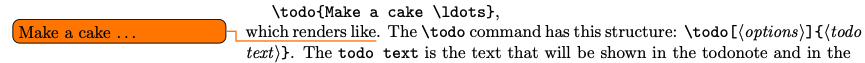
\includegraphics[width=\linewidth]{images/todo}
\end{frame}

\begin{frame}[fragile]
    \frametitle{siunitx -- Tabellen}
    \begin{lstlisting}[basicstyle=\ttfamily\footnotesize]
\usepackage{siunitx} % Preamble
\begin{tabular}{@{}l S[table-format=4.3] S[table-format=1e+1]@{}}
    \toprule
    Name        & {Zahl} & {Exponent} \\ \midrule
    Tausend     & 1000   & 1e3        \\
    Zehn        & 10     & 1e1        \\
    Hunderstel  & 0.01   & 1e-2       \\
    Tausendstel & 0.001  & 1e-3       \\ \bottomrule
\end{tabular}
    \end{lstlisting}
    \vspace*{-1ex}
    \begin{center}
        \begin{tabular}{@{}l S[table-format=4.3] S[table-format=1e+1]@{}}
            \toprule
            Name        & {Zahl} & {Exponent} \\ \midrule
            Tausend     & 1000   & 1e3        \\
            Zehn        & 10     & 1e1        \\
            Hunderstel  & 0.01   & 1e-2       \\
            Tausendstel & 0.001  & 1e-3       \\ \bottomrule
        \end{tabular}
    \end{center}
\end{frame}

\begin{frame}[fragile]
    \frametitle{newcomputermodern}
    \begin{multicols}{2}
        \small\justifying{\fontspec{LMRoman10-Regular}
            Als Gregor Samsa eines Morgens aus unruhigen Träumen erwachte, fand er sich in seinem Bett zu einem ungeheueren Ungeziefer verwandelt.
            Er lag auf seinem panzerartig harten Rücken und sah, wenn er den Kopf ein wenig hob, seinen gewölbten, braunen, von bogenförmigen Versteifungen geteilten Bauch, auf dessen Höhe sich die Bettdecke, zum gänzlichen Niedergleiten bereit, kaum noch erhalten konnte.
        }

        Als Gregor Samsa eines Morgens aus unruhigen Träumen erwachte, fand er sich in seinem Bett zu einem ungeheueren Ungeziefer verwandelt.
        Er lag auf seinem panzerartig harten Rücken und sah, wenn er den Kopf ein wenig hob, seinen gewölbten, braunen, von bogenförmigen Versteifungen geteilten Bauch, auf dessen Höhe sich die Bettdecke, zum gänzlichen Niedergleiten bereit, kaum noch erhalten konnte.
    \end{multicols}
    \begin{itemize}
        \item Book Weight
        \item Unicode (ελληνική Україна ⠅⠆⠇⠝⠞ \smash{x̧̗̖̀́̃̂} ☭ Ⳃ ʛ)
    \end{itemize}
\end{frame}

\begin{frame}[fragile]
    \frametitle{latexindent}
    \begin{lstlisting}[basicstyle=\ttfamily\scriptsize]
\begin{tabular}{@{}lccc@{}}                                  \toprule
    Name      & \multicolumn{3}{@{}c@{}}{Charakteristika} \\ \cmidrule{2-3}
              & Groß & Haarig & Süß                       \\ \midrule
    Aprikose  & Nein & Nein   & Ja                        \\
    Nektarine & Ja   & Ja     & Ja                        \\
    Pfirsich  & Ja   & Nein   & Ja                        \\ \midrule
    ???       & Nein & Ja     & ???                       \\
    Gorilla   & Ja   & Ja     & Ja                        \\ \bottomrule
\end{tabular}
    \end{lstlisting}
    \begin{itemize}
        \item Automatisches Einrücken von Environments;
        \item Automatisches Einrücken nach Items;
        \item Alignment in Tabellen.
        \item Setup ist \textsc{pita}.
    \end{itemize}
\end{frame}

% == == == == == == == == == == == == == == == == == == == == == == == == == == == ==
\appendix
\miniframesoff
\begin{frame}[fragile]
    \frametitle{Dankeschön}
    \note{Fragen / Ergänzungen?}
    \note{Sticker}
    Immer nach spezifischen Anforderungen und Styleguides fragen!\\\vfill

    \pause

    \begin{tabularx}{\linewidth}{@{}CCC@{}}
        Slides                                                       & Website                                   & Mastodon                                                    \\
        \qrcode[hyperlink,version=5]{github.com/kamik423/latex-talk} & \qrcode[hyperlink,version=5]{hans.coffee} & \qrcode[hyperlink,version=5]{mastodon.social/@SherlockHans} \\
        \url{github.com/kamik423/latex-talk}                         & \url{hans.coffee}                         & \url{mastodon.social/@SherlockHans}                         \\
    \end{tabularx}

\end{frame}

\end{document}
